%for a more compact document, add the option openany to avoid
%starting all chapters on odd numbered pages
\documentclass[12pt,openany]{cmuthesis}

% This is a template for a CMU thesis.  It is 18 pages without any content :-)
% The source for this is pulled from a variety of sources and people.
% Here's a partial list of people who may or may have not contributed:
%
%        bnoble   = Brian Noble
%        caruana  = Rich Caruana
%        colohan  = Chris Colohan
%        jab      = Justin Boyan
%        josullvn = Joseph O'Sullivan
%        jrs      = Jonathan Shewchuk
%        kosak    = Corey Kosak
%        mjz      = Matt Zekauskas (mattz@cs)
%        pdinda   = Peter Dinda
%        pfr      = Patrick Riley
%        dkoes = David Koes (me)

% My main contribution is putting everything into a single class files and small
% template since I prefer this to some complicated sprawling directory tree with
% makefiles.

% some useful packages
\usepackage{tgpagella}
\usepackage{fullpage}
\usepackage{graphicx}
\usepackage{amsmath}
\usepackage[numbers,sort]{natbib}
\usepackage[backref=false,pageanchor=true,plainpages=false, pdfpagelabels, bookmarks,bookmarksnumbered,
%pdfborder=0 0 0,  %removes outlines around hyper links in online display
]{hyperref}
% \usepackage{subfigure}

% Approximately 1" margins, more space on binding side
%\usepackage[letterpaper,twoside,vscale=.8,hscale=.75,nomarginpar]{geometry}
%for general printing (not binding)
\usepackage[letterpaper,twoside,vscale=.8,hscale=.8,nomarginpar,hmarginratio=1:1]{geometry}

\usepackage{amsmath,amsfonts,bm}
\usepackage{booktabs} % For formal tables
\usepackage{graphicx}
\usepackage{graphics}
\usepackage{array}
\usepackage{color}
\usepackage{xcolor}
\usepackage{colortbl}
\usepackage{makecell}
\usepackage{multirow}
\usepackage{arydshln}
\usepackage{xspace}
\usepackage{subcaption}
\usepackage{caption}
\usepackage{algpseudocode}
\usepackage[noend,ruled]{algorithm2e}
\usepackage{setspace}
\usepackage{varwidth}
\usepackage{enumitem}
\usepackage{mdframed}
\usepackage{centernot}
\usepackage{textcomp}
\usepackage{soul}
\usepackage{pifont}
\usepackage{wrapfig}
\usepackage{url}
\usepackage{hyperref}
\usepackage[nameinlink]{cleveref}
\usepackage{cuted}
\usepackage{tcolorbox}
\tcbuselibrary{breakable}
\usepackage{lipsum}
\usepackage{listings}
\usepackage{twemojis}
\usepackage[T1]{fontenc}

\usepackage{tikz}
\usetikzlibrary{positioning}

\newcounter{timelineitem}
\newcommand{\timelineentry}[2]{%
  \stepcounter{timelineitem}%
  \node[circle,fill=black,inner sep=2pt] (dot\thetimelineitem) at (0,-\value{timelineitem}) {};
  \node[anchor=west] at (0.7,-\value{timelineitem}) {#1};
  \node[anchor=west] at (5.8,-\value{timelineitem}) {#2};
  \ifnum\value{timelineitem}>1
    \draw[thin] (dot\number\numexpr\value{timelineitem}-1\relax) -- (dot\thetimelineitem);
  \fi
}

\newcommand{\cmark}{\ding{51}}%
\newcommand{\xmark}{\ding{55}}%

\newcommand{\cmtransours}{CMTrans\xspace}
\newcommand{\CC}{Comp-Corp\xspace}

\newcommand{\repostmethodName}{\textsc{RepoST}\xspace}
\newcommand{\repostdatasetName}{\textsc{RepoST}\xspace}
\newcommand{\reposttrainsetName}{\textsc{RepoST-Train}\xspace}
\newcommand{\repostevalsetName}{\textsc{RepoST-Eval}\xspace}

\newcommand{\anchordrours}{Anchor-DR\xspace}

\newcommand{\repostmethodname}{\textsc{Hybrid-Gym}\xspace}

\newcommand{\fencemodelname}{\textsc{FenCE}\xspace}

\newcommand{\plusname}{\textsc{Hybrid-Plus}\xspace}

\newcommand{\proposedWork}{\textbf{\textcolor{treegreen}{proposed work}}}

% circled
\newcommand{\circled}[1]{\textcircled{\raisebox{-0.9pt}{#1}}}



% newly added
\newcommand{\edit}[1]{\textcolor{darkgreen}{#1}}

\newcommand{\TBD}[1]{\textcolor{blue}{[TBD: #1]}}
\newcommand{\yiqing}[1]{\textcolor{blue}{[Yiqing: #1]}}
\newcommand{\daniel}[1]{\textcolor{brown}{[Daniel: #1]}}

\newcommand{\plan}{\textcolor{blue}{[Plan]}}

\newcommand{\ie}{\textit{i.e.},} % that is
\newcommand{\eg}{\textit{e.g.},} % for example
\newcommand{\start}[1]{\vspace{1.5mm}\noindent{{\bf #1}.}}
\DeclareMathOperator*{\argmin}{arg\,min\,}
\DeclareMathOperator*{\argmax}{arg\,max\,}
\newcommand\numberthis{\addtocounter{equation}{1}\tag{\theequation}}


% defining vspace 
\newcommand{\downv}{\vspace{-.0cm}}
\newcommand{\upv}{\vspace{-.0cm}}
% \newcommand{\downve}{\vspace{-.0cm}}


% \usepackage{color, colortbl}
\definecolor{amber}{rgb}{1.0, 0.75, 0.0}
\definecolor{applegreen}{rgb}{0.55, 0.71, 0.0}
\definecolor{treegreen}{rgb}{0.13, 0.54, 0.23}
\definecolor{LightCyan}{rgb}{0.88,1,1}
\definecolor{LightBlue}{RGB}{171, 227, 235}
\newcommand{\bad}{\cellcolor{red!8}}
\newcommand{\worse}{\cellcolor{red!16}}
\newcommand{\good}{\cellcolor{applegreen!10}}
\newcommand{\better}{\cellcolor{applegreen!20}}
\newcommand{\hlcell}{\cellcolor{applegreen!22}}
\newcommand{\hlrow}{\rowcolor{amber!18}}
\newcommand{\dlrow}{\rowcolor{gray!20}}
\newcommand{\sdlrow}{\rowcolor{gray!10}}
\newcommand{\blrow}{\rowcolor{LightBlue!30}}
\newcommand{\dlcell}{\cellcolor{gray!20}}



\definecolor{green2}{HTML}{BFD8B6}
\definecolor{green3}{HTML}{E7F0E5}
\definecolor{greenarrow}{HTML}{1DB100}
\definecolor{red3}{HTML}{C82506}

% defining colours to be used in figures
% \definecolor{gred}{RGB}{219,68,55}
\definecolor{gred}{RGB}{255,102,102}
\definecolor{gblue}{RGB}{51,102,255}
\definecolor{gyellow}{RGB}{244,180,0}
\definecolor{ggreen}{RGB}{15,157,88}
\definecolor{ggrey}{RGB}{115,115,115}
\definecolor{na}{gray}{0.9}

\definecolor{textRed}{RGB}{157,0,23}
\definecolor{textYellow}{RGB}{166,119,54}
\definecolor{textGreen}{RGB}{58,110,38}
\definecolor{textBlue}{RGB}{39,71,156}

% \definecolor{lightRed}{RGB}{255,222,222}
% \definecolor{lightYellow}{RGB}{255,255,193}
% \definecolor{lightGreen}{RGB}{222,255,222}
% \definecolor{lightBlue}{RGB}{221,231,244}

\definecolor{LightYellow}{RGB}{255,250,208}
\definecolor{LightGreen}{RGB}{194,255,192}
\definecolor{LightBlue}{RGB}{187,236,251}
\definecolor{LightPurple}{RGB}{224,223,255}
\definecolor{LightGrey}{RGB}{225,225,225}

\definecolor{OrangeRed}{rgb}{1.0, 0.27, 0.0}
\definecolor{mediumgreen}{RGB}{72, 158, 52}
\definecolor{darkgreen}{rgb}{0.0, 0.42, 0.24}
\definecolor{midnightgreen}{rgb}{0.0, 0.29, 0.33}
\definecolor{aquablue}{RGB}{52, 147, 158}

\definecolor{diagramRed}{RGB}{246,193,193}
\definecolor{diagramPurple}{RGB}{224,224,253}
\definecolor{diagramOrange}{RGB}{244,222,176}
\definecolor{diagramGrey}{RGB}{236,236,236}

\definecolor{Grey}{RGB}{150,150,150}

\newcommand{\ctext}[2]{%
  \begingroup
  \sethlcolor{#1}%
  \hl{ #2 }%
  \endgroup
}

\newcommand{\hlpgen}[2]{\fboxsep1pt \colorbox{ggreen!#2}{\strut #1}} % highlight text with custom saturation. for pgen
\newcommand{\hlcov}[2]{\fboxsep1pt \colorbox{gyellow!#2}{\strut #1}} % highlight text with custom saturation. for cov
\newcommand{\colorR}[1]{\textcolor{gred}{\textbf{#1}}}
\newcommand{\colorG}[1]{\textcolor{ggreen}{\textbf{#1}}}
\newcommand{\colorB}[1]{\textcolor{gblue}{\textbf{#1}}}
\newcommand{\colorGrey}[1]{\textcolor{ggrey}{\textbf{#1}}}

\newcommand{\colorr}[1]{\textcolor{gred}{#1}}
\newcommand{\colorg}[1]{\textcolor{ggreen}{#1}}
\newcommand{\colorb}[1]{\textcolor{gblue}{#1}}

\newcommand{\colordg}[1]{\textcolor{darkgreen}{#1}}
\newcommand{\colorgrey}[1]{\textcolor{Grey}{#1}}

% Provides a draft mark at the top of the document. 
\draftstamp{\today}{DRAFT}

\begin {document} 
\onehalfspacing
\frontmatter

%initialize page style, so contents come out right (see bot) -mjz
\pagestyle{empty}

\title{ %% 
{\it Thesis Proposal} \\
{\bf Synthetic Training Data Construction for Coding Agents}
}
\author{Yiqing Xie}
% \date{January 3006}
\Year{2026}
\trnumber{}

\committee{
Carolyn Rosé, Chair \\
Daniel Fried \\
Graham Neubig \\
Dan Roth
}

\support{}
\disclaimer{}

% copyright notice generated automatically from Year and author.
% permission added if \permission{} given.

\keywords{synthetic data, coding agent, code generation}

\maketitle

% \begin{dedication}
% For my dog
% \end{dedication}

% \pagestyle{plain} % for toc, was empty

\begin{abstract}
With the development of AI techniques, the role of AI in software development is shifting from script-level, static code generation to project-level coding agents.
This dissertation research focuses on the fundamental challenges of training coding agents: the high cost of constructing training data, the difficulty of handling diverse use cases simutaneously, and the performance saturation with respect to data scale.
To this end, this thesis is structured around three parts: (1) constructing scalable training data, (2) improving the generalizability of coding agents, and (3) training critique models for coding agents.

One major bottleneck of scaling coding agent training data is the construction of training environments, which are abstractions of real-world coding setups.
Building the environments can require substantial human or agent effort, for example, when the environments support the executability and unit testing of an entire code repository. 
In our work, we aim to find an appropriate level of abstraction for training environments, with the goal of simplifying their construction while preserving training effectiveness.

Building on this lightweight environment construction process, we extend coding agents' abilities to diverse downstream coding tasks. In particular, we develop principles for designing synthetic training tasks and characterize atomic skills that transfer across coding tasks. Our work bridges the gap between single-task training and general-purpose coding agent training.

Even with these advances in coding agent training, empirically, we observe that for a specific model, additional training data yields little or no further gain after a certain point.
Our analysis further shows that the performance is substantially bottlenecked by the limited high-level planning ability: producing intermediate steps about what should be done and in what order, as opposed to low-level implementation: generating concrete executable actions to perform the intermediate steps.
In our work, we aim to train an additional critique model that specializes in planning and dynamically provides guidance to the coding agent in inference.

Together, this thesis aims to build scalable data to train effective coding agents and critique models that generalize across diverse coding tasks.
\end{abstract}

% \begin{acknowledgments}
% TBD.
% \end{acknowledgments}



\tableofcontents
\listoffigures
\listoftables

\mainmatter

%% Double space document for easy review:
%\renewcommand{\baselinestretch}{1.66}\normalsize

% The other requirements Catherine has:
%
%  - avoid large margins.  She wants the thesis to use fewer pages, 
%    especially if it requires colour printing.
%
%  - The thesis should be formatted for double-sided printing.  This
%    means that all chapters, acknowledgements, table of contents, etc.
%    should start on odd numbered (right facing) pages.
%
%  - You need to use the department standard tech report title page.  I
%    have tried to ensure that the title page here conforms to this
%    standard.
%
%  - Use a nice serif font, such as Times Roman.  Sans serif looks bad.
%
% Other than that, just make it look good...



\chapter{Introduction}
With the rapid advancement of AI techniques, the role of AI in software development is evolving from script-level, static code generation toward project-level coding agents. 
Unlike traditional code assistants that are lmited to producing isolated snippets of code, coding agent infra-structures such as SWE-Agent~\cite{sweagent} and OpenHands~\cite{openhands} provide tools for the LLM to understand broader repository context, track dependencies across files, develop multi-step development plans, etc. 
This enables them to assist with more complex tasks such as feature implementation, refactoring, debugging, testing, and maintenance of the entire codebase.

\begin{figure}[h]
  \centering
  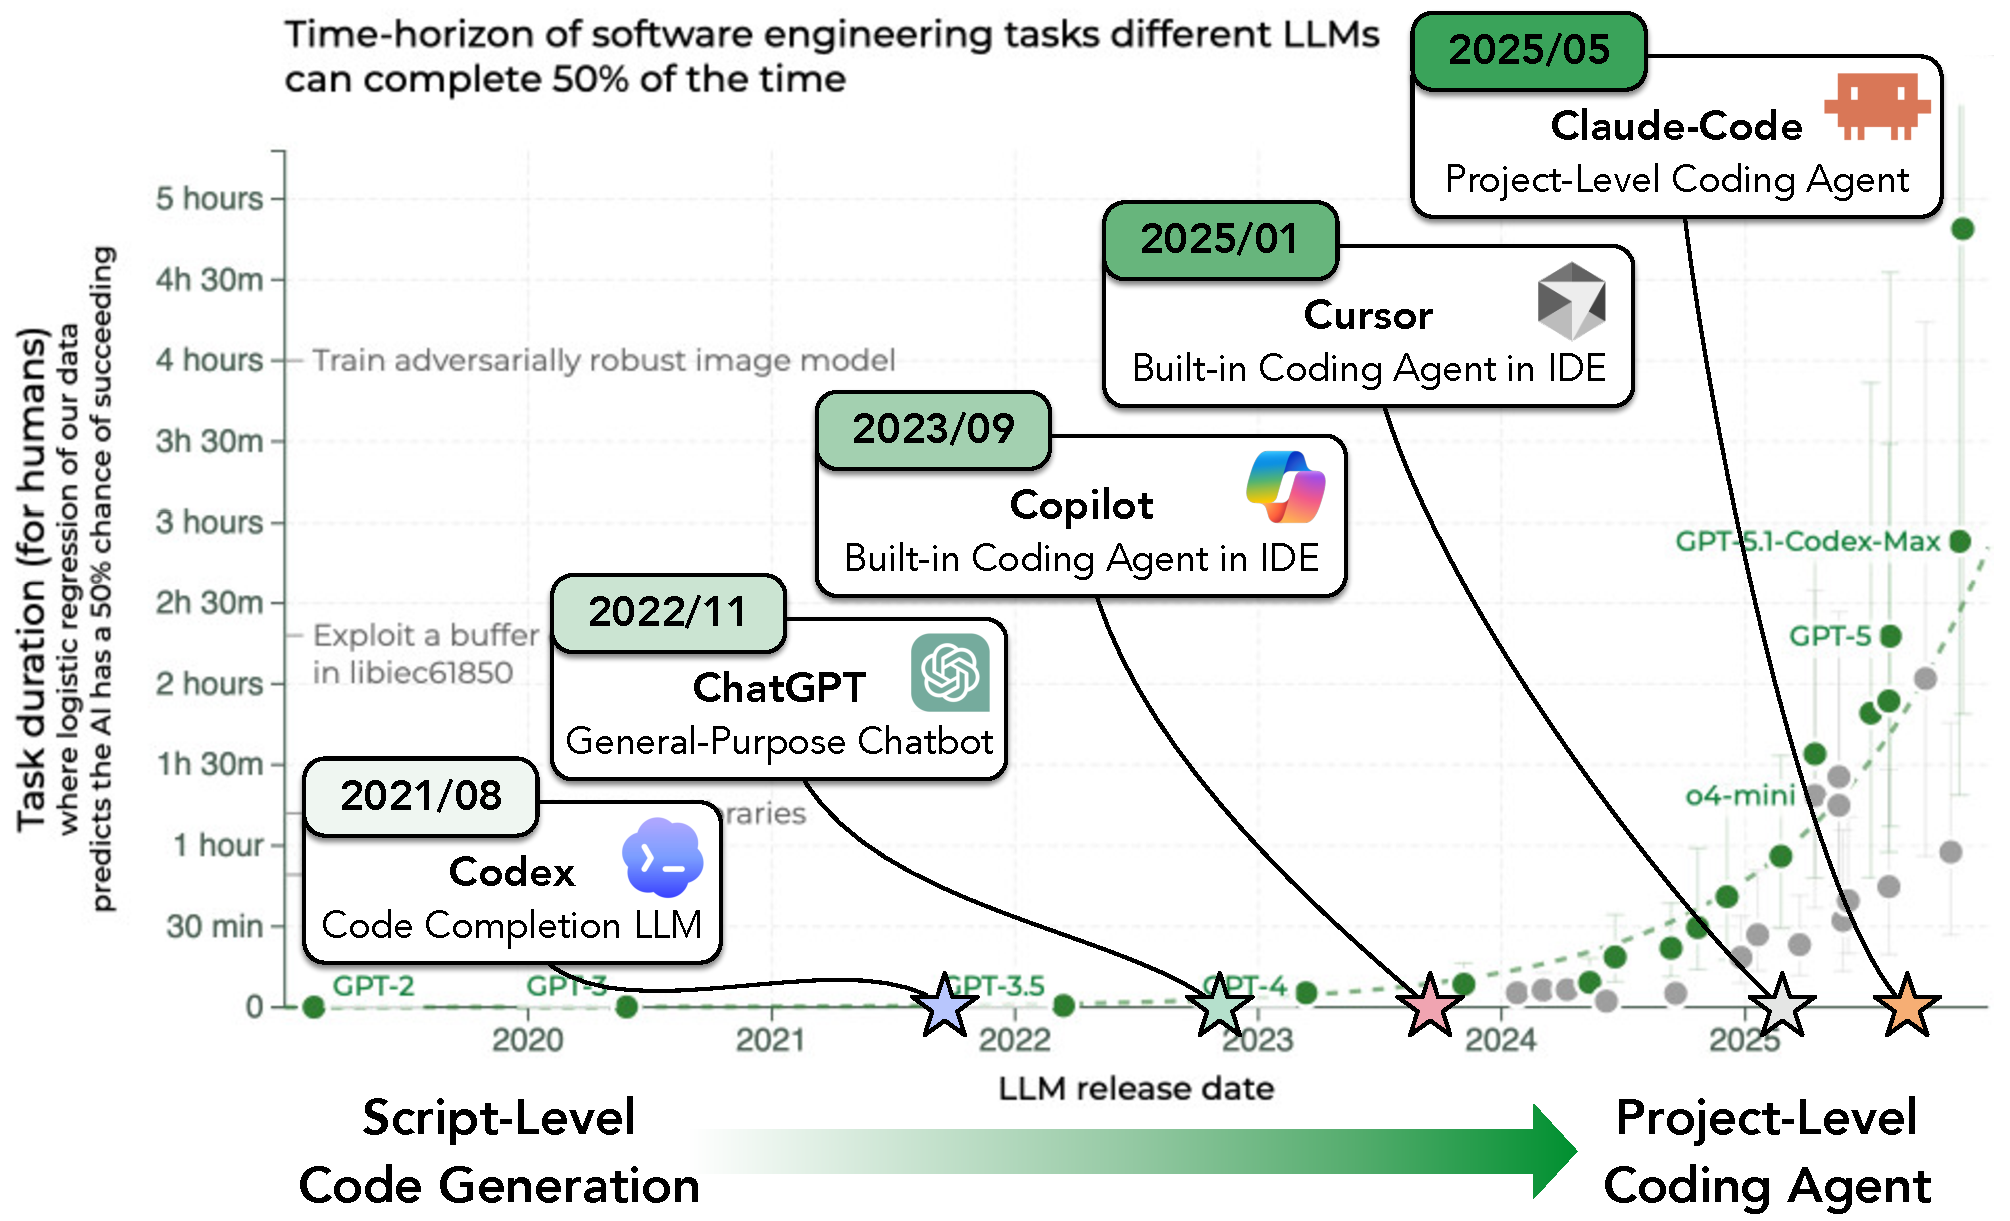
\includegraphics[width=0.8\linewidth]{figs/proposal_intro.pdf}
  \caption{The timeline of how the paradigm of the collaboration between human and AI coding assistants shifts from script-level static code generation to project-level coding agent.}
  \label{fig:proposal_intro}
\end{figure}

Although coding agents have shown strong performance on recent benchmarks that simulate real-world scenarios, there remains substantial room to improve both the effectiveness and feasibility of coding agent training.
We identify several fundamental challenges as follows:

\start{The High Cost of Constructing Training Data}
Although the scale of training data has been shown to be a major factor in coding agent performance~\cite{swe-smith}, constructing such data remains highly expensive.
One major bottleneck is the construction of training environments that serve as abstractions of real-world coding setups, which typically involve docker environments with all required external packages installed, test suites for major features in a codebase, etc. 
Given the current state of LLM capacity, this process still demands substantial human or agent effort~\cite{swe-smith}.
Such resources are particularly scarce in academia, where the engineering, computational, human, and financial resources are often limited, hindering the development of systematic research on coding agent training.

\start{The Difficulty of Handling Diverse Use Cases Simutaneously}
In real-world deployment, coding agents must operate across diverse tasks and scenarios, and can be paired with different tools, execution harnesses, and inference-time techniques.
However, most existing research still focuses on training agents for a single task under a fixed inference setting and with a predefined set of tools, which does not reliably generalize to other settings~\cite{swe-play}.
What still remains underexplored is how well skills transfer across these dimensions and how such transferability can be improved.
Such lack of understanding creates a significant gap between current coding agent research and practical real-world applications.

\start{The Performance Saturation with Respect to Data Scale}
% Even if the first two challenges are addressed, the performance of coding agents is still fundamentally constrained by the capacity of the underlying base models.
% On one hand, this is an inherent challenge of machine learning, where a model's ability to fit mapping functions and represent patterns is limited.
% Such limitation is especially pronounced for coding agent training, which requires complex and diverse skills from multiple aspects, including tool usage, coding-related knowledge, instruction-following, etc.
% On the other hand, training models with larger sizes is again bottlenecked by the computational resources, which is particularly limited in academia.
Even if the first two challenges are addressed, empirically, we observe that for a specific model, especially the one with limited size (e.g., Qwen2.5Coder-7B and 14B~\cite{qwen25coder}), increasing the size of training data yields little or no further gain after a certain point~\cite{swe-smith,R2EGym}.
To better understand this limitation, we break down the abilities required for coding agent training into high-level planning (producing intermediate steps about what should be done and in what order) and low-level implementation (generating concrete executable actions to perform the intermediate steps).
Our analysis suggests that high-level planning remains a major bottleneck: even after training, there is still a substantial gap between these models and frontier models such as Claude Sonnet 4.6~\cite{claude46}.
Although increasing the size of the base model can raise the performance ceiling, it also requires more computational resources, which is particularly limited in academia.

In this thesis, we aim to mitigate the three challenges by (1) constructing scalable training data, (2) improving the generalizability of coding agents, and (3) training critique models to assist coding agents.

\section{Thesis Overview}
This thesis contains three parts targeting the three above challenges, respectively.

\start{Part 1: Coding Agent Training with Scalable Synthetic Data}
As abstractions of real-world coding setups, training environments are typically complex and require substantial human or agent effort to construct.
In our work, we aim to find an appropriate level of abstraction for training environments.
Specifically, we identify the execution support for the entire codebase to be the major bottleneck of training environment construction, and propose training settings that avoid code execution or only require execution for a particular module in the codebase.
This simplifies the construction of training environments while preserving training effectiveness.

\start{Part 2: Training Coding Agents that Generalize across Tasks}
Most existing coding agent training datasets only focus on a single task, which does not reliably generalize to other tasks.
In our work, we open a direction of training coding agents that generalize across tasks.
Specifically, we conduct systematic analyses on the commonalities shared across diverse downstream coding tasks, and design synthetic training tasks that can generalize across tasks.
In the \textbf{\textcolor{treegreen}{proposed work}}, we take a step forward and analyze the exact trajectory behaviors (including problem-solving strategies and concrete actions) that are transferrable across tasks. Then we propose a data selection method based on such desired behaviors beyond task success.

\start{Part 3: Training Critique Models to Assist Coding Agent}
While the first two parts aim to improve the effectiveness of coding agent training, empirically, we still observe that the performance satuates with respect to data scale after a certain point, and the high-level planning ability remains a major bottleneck.
To address this limitation, in our work, we develop critique models that provide guidance to the coding agent at inference time.
Compared to the coding agent that is optimized for the combination of high-level planning and low-level implementation, the critique model is specialized in planning.
We first show that the high-level idea of ``training a specialized model to provide guidance to the main model'' can be beneficial in general NLP tasks such as factuality generation.
Then in the \textbf{\textcolor{treegreen}{proposed work}}, we apply this idea to coding agent training and train critique models to assist coding agents in inference.
We show that there is a large room of improvement for training critique models for coding agents, and propose a recipe to train critique models.

\newpage
\section{Proposed Timeline}

\begin{figure}[h!]
    \centering
    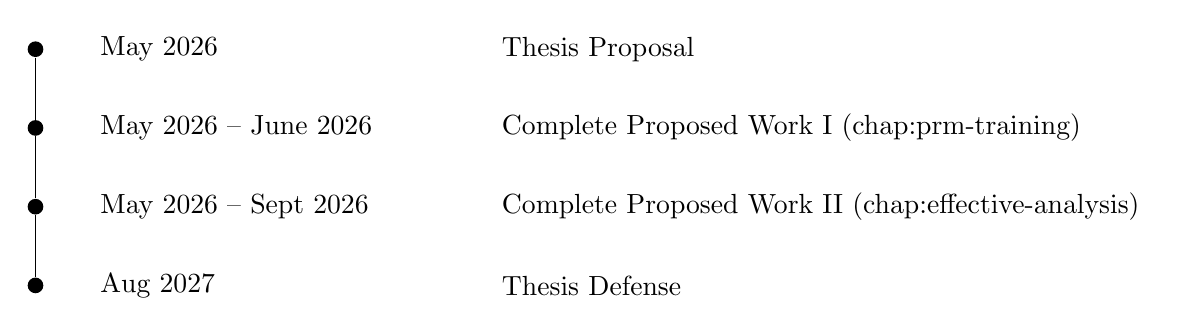
\begin{tikzpicture}
    
    \setcounter{timelineitem}{0}
    \timelineentry{May 2026}{Thesis Proposal}
    \timelineentry{May 2026 -- June 2026}{Complete Proposed Work I (\autoref{chap:prm-training})}
    \timelineentry{May 2026 -- Sept 2026}{Complete Proposed Work II (\autoref{chap:effective-analysis})}
    \timelineentry{Aug 2027}{Thesis Defense}
\end{tikzpicture}
\end{figure}






\chapter{Literature Review}
% 80-20 rule: 80: easy solutions; 20: the residule
% Overall goal: make coding agent training more feasible.
% 1. make scalable data: 
%     - existing work: datasets
%     - what's missing: it is still challenging and expensive to construct synthetic training data

% 2. what's missing in part 1: generalizability of coding agents 
%     - existing work: general-purpose agent training 
%     - what's missing: mid-training (general-purpose coding agent training)

% 3. what's missing in part 1 and 2: the limitation of coding agent training
%     - existing work: how critique models could be helpful 
%     - what's missing: understanding what kind of critique is helpful

The structure of this chapter is as follows: 
In \S\ref{sec:related-overview}, we introduce the overview of coding agent training. 
In \S\ref{sec:related-scalable}, we discuss existing work that constructs scalable training data, and introduce how our work opens a direction of constructing scalable coding agent training data with lightweight environments.
Since most coding agent training datasets only focus on a single task, to train coding agents that are capable across a diverse set of applications, in \S\ref{sec:related-generalizability}, we further discuss the generalizability of coding agents, where our work aims to reveal the key abilities that are transferrable across different coding tasks.
While all the above works show effective ways to directly train coding agents, the performance is still bottlenecked by the capacity of the base models. To address this limitation, in \S\ref{sec:related-critique}, we discuss how existing work uses inference-time feedback to improve LLM generation, and how we apply this idea to coding agent and train critique models to assist coding agents in inference.




\section{Coding Agent Overview}
\label{sec:related-overview}
\subsection{Benchmarks for Coding Agents}
Coding agents have shown strong performance on recent repository-level benchmarks.
The SWE-Bench issue-solving benchmark~\cite{swebench} evaluates the ability to resolve a GitHub issue in a real-world repository by generating a code patch.
Following SWE-Bench, SWE-bench Pro~\cite{swebench-pro} is a more challenging issue-solving benchmark that captures realistic, complex, enterprise-level problems beyond the scope of SWE-Bench.
Similarly, SWE-bench Multimodal~\citep{swebench-multimodal} further targets visual, user-facing software domains and includes multimodal context (e.g., images) in issue-solving.
Multi-SWE-bench~\citep{multi-swe-bench} extends the issue-resolution setting to repositories to nine different programming languages.

Beyond issue-solving benchmarks, SWT-Bench~\cite{swt-bench} and TestGenEval~\cite{testgeneval} target test generation, where the goal is to generate a set of test functions for a GitHub issue.
Commit-0~\cite{commit0} evaluates the ability to generate the entire library from scratch. The results will be evaluated by the number of tests passed.
ArtifactsBench~\cite{artifactsbench} assesses the transformation from multimodal instructions into high-quality and interactive visual artifacts.
SWE-Perf~\cite{sweperf} and SWE-fficiency~\cite{swefficiency} evaluate the ability to improve code efficiency (i.e., execution time) in addition to correctness.
KernelBench~\cite{kernelbench} targets the generation of GPU kernels.
SUPER~\cite{super}, EnvBench~\cite{envbench}, and TerminalBench~\cite{terminalbench} evaluate the agent's ability to run bash commands for setup and execution tasks.
Multiple benchmarks are focusing on function generation~\cite{classeval,repocoder,codereval,evocodebench,deveval,R2E,repost}. Given the description of the function, the task is to complete the function body.
All these benchmarks are designed to simulate real-world use cases for coding agents and require repository exploration and patch-style edits.

\subsection{Coding Agent Infrastructure}
Approaches to solving the above benchmarks include workflow-based pipelines and agent frameworks. 
Workflow-based systems explicitly structure the solution process into stages, as in Agentless~\cite{agentless}.
In comparison, coding agents can dynamically call tools to interact with the environment, enabling end-to-end problem solving.

Agent infrastructure such as SWE-Agent~\cite{sweagent} and OpenHands~\citep{openhands} provide agent-computer interfaces for tool use and editing. 
SWE-Agent introduces the concept of agent-computer interface: a structured set of interactions for searching/navigating code, viewing and editing files, and executing commands/tests, all with careful context management.
Building upon SWE-agent, mini-SWE-Agent~\cite{sweagent} achieves similar performance with a simpler control flow.
Live-SWE-agent explores online self-evolution of SWE agents~\citep{live-swe-agent}. 
SWE-Search~\citep{swe-search} improves SWE-Agent using planning (e.g., Monte Carlo Tree Search) with iterative refinement. 
Compared to SWE-Agent, OpenHands~\cite{openhands} provides a wider range of tools that allow the agent to interact with the world in similar ways to those of a human developer: by writing code, interacting with a command line, and browsing the web.

\subsection{Training Paradigms for Coding Agent}
To train coding agents, SWE-Gym~\cite{swegym} adopts rejection sampling finetuning, which applies a teacher model to generate trajectories, evaluates the correctness, and finetunes the student model on the successful trajectories.
SWE-RL~\cite{swerl} trains the agent model with reinforcement learning, with the similarity score between ground-truth and LLM-generated solutions as reward.
A follow-up work, ML-Agent~\cite{mlagent}, extends SWE-RL with exploration-enriched fine-tuning, step-wise RL, and an agentic ML-specific reward module.



\section{Scalable Coding Agent Training}
\label{sec:related-scalable}
We focus on the training of end-to-end coding agents in this section.
As shown in multiple existing works~\citep{swegym,R2EGym,swe-smith}, the performance of coding agents significantly improves when we scale up the training data, especially for base models with larger sizes. For instance, SWE-Smith show that the performance of coding agents with Qwen2.5Coder-32B~\cite{qwen25coder} as the base model is still not converged when we have around 5k training trajectories.

Towards this challenge, existing works focus on reducing the effort of constructing training data.
SWE-Gym~\cite{swegym} presents the first set of training environments for coding agents. The authors manually construct training environments using the same approach as SWE-Bench~\cite{swebench}. Each training environment contains a GitHub issue, the ground truth code patch to resolve it, and the corresponding GitHub snapshot with all required packages installed, which is equipped with the test function for the issue. The resulting dataset has 491 training trajectories.
Following SWE-Gym, to reduce the effort of constructing training environments, R2E-Gym~\cite{R2EGym} improves the scalability of executable training environments by using test-generation and back-translation directly from commits. Although it still requires human effort to set up the repositories, it reduces the reliance on human-written issues or unit tests and thereby improves the training data scale to 3.3k trajectories.
A concurrent work, SWE-Smith~\cite{swe-smith} generates scalable executable environments at a scale by automatically synthesizing bugs, which obtains 5.0k training trajectories. The authors also reduce the number of dockers in the training dataset by keeping only one docker image for each repository.
The only part that requires human effort is the installation of repositories, where the authors explicitly mention that it is necessary to have human agent collaboration to ensure installation success rate.
SWE-Play~\cite{swe-play} reduces human effort with a completely automatic approach. It uses a coding agent to propose training tasks, build the repositories from scratch, implement the tasks, and generate tests to verify the correctness. Although it avoids human effort, the environment construction process is still challenging and expensive for agents to complete, resulting a dataset with only 704 training trajectories.

There is still a large room of improvement for constructing scalable training data. Particularly, existing works either still require human effort in repository setup or test generation, or suffer from low success rates with a fully automatic approach.
One potential reason is that they use the same executability setting in training and in downstream evaluation. Specifically, they require the repository to be executable, which encourages code execution and verification in training trajectories and enables unit-testing to select successful trajectories.
In our work, we investigate: to what extent can training environments without executable repositories still be effective for coding agent training?
We will answer this question by analyzing the effect of executability in coding tasks and constructing unit-testing without executable repositories.



\section{Generalizability of Coding Agents}
\label{sec:related-generalizability}
\TBD{Here we introduce existing work on general-purpose agent training, where coding tasks are only a subset of training tasks.}
In the pre-training stage, recent work train the language models on general agentic tasks, including proprietary models~\cite{gpt5,claude37,claude45} and open-sourced ones~\cite{deepseekv3,kimik2,qwen25coder,qwen3,llama3modelcard}.
For instance, Kimi-K2~\cite{kimik2} constructs a wide range of synthetic tools and tasks to boost general agentic abilities.


\TBD{What's specifical about our work: (1) we focus on general-purpose coding agent training, which is a stage between pre-training and single-task post-training; (2) we aim to reveal the key abilities that are transferrable across different coding tasks.}




\section{Training Critique Models for Coding Agent}
\label{sec:related-critique}
\TBD{Here we introduce existing work on improving the planning ability of coding agents, especially on multi-agent systems}

\TBD{Showing what's special about critique model training: can combine with any existing coding agents.}







\part{Coding Agent Training with Scalable Synthetic Data}
\label{part:scalability}


\start{Overview of Part~\ref{part:scalability}}
This part comprises two chapters organized around a single theme: \emph{by reducing the complexity of constructing training data in appropriate ways, we could potentially improve scalability while preserving effectiveness}.
 
Chapter~\ref{chap:cmtrans} illustrates this idea through a code translation task. A key bottleneck of the scale of training data is the difficulty of obtaining parallel data pairs (i.e., functionally equivalent code written in different programming languages).
To address this, we show that constructing comparable code pairs (i.e., code snippets with similar functionality) is substantially easier, and that training on such pairs remains effective. Experiments further demonstrate that combining comparable and parallel data significantly outperforms training on parallel data alone.

Chapter~\ref{chap:repost} applies the same principle to training coding agents. Here, the primary bottleneck is constructing the training environment: typical workflows require installing an entire repository (on average 26.5 external packages), which demands substantial effort from both humans and agents. We mitigate this challenge by bypassing repository installation via sandbox testing, which greatly simplifies environment construction (by installing only 2.1 packages per instance). Importantly, the resulting training examples remain effective because the agent can still access the full repository when completing the task.

% Chapter~\ref{chap:effective-analysis} outlines a proposed work aimed at empirically answering the question: “what makes a training trajectory effective” for coding agents. We first show that even successful trajectories on the same set of instances can vary widely in effectiveness. We then propose to identify the characteristics that distinguish trajectories generated by different teacher models.
% Finally, we propose to improve trajectory effectiveness by injecting beneficial characteristics into training trajectories.




\chapter{Constructing Scalable Code Translation Training Data with Comparable Corpora and Multiple References \textcolor{aquablue}{(\textit{completed})}}
\label{chap:cmtrans}


\newcommand{\hlours}[1]{%
  \begingroup
  \sethlcolor{#1}%
  \hl{ CMTrans }%
  \endgroup
}

\begin{figure}[t]
    \centering
    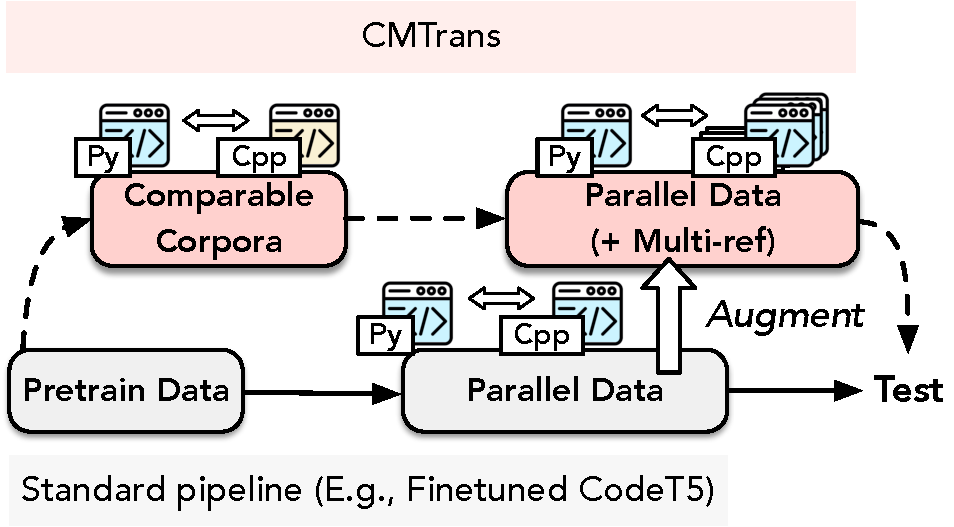
\includegraphics[width=0.5\linewidth]{CMTrans_figs/diagram_intro_v2.pdf}
    \caption{The standard pipeline for code translation (colored in light grey) and the CMTrans pipeline (colored in pink). The comparable corpora are both naturally occurring and model generated. We generate multiple references by \cmtransours.
    }
    \label{fig:cmtrans_diagram_intro}
\end{figure}

\begin{figure}[t]
    \centering
    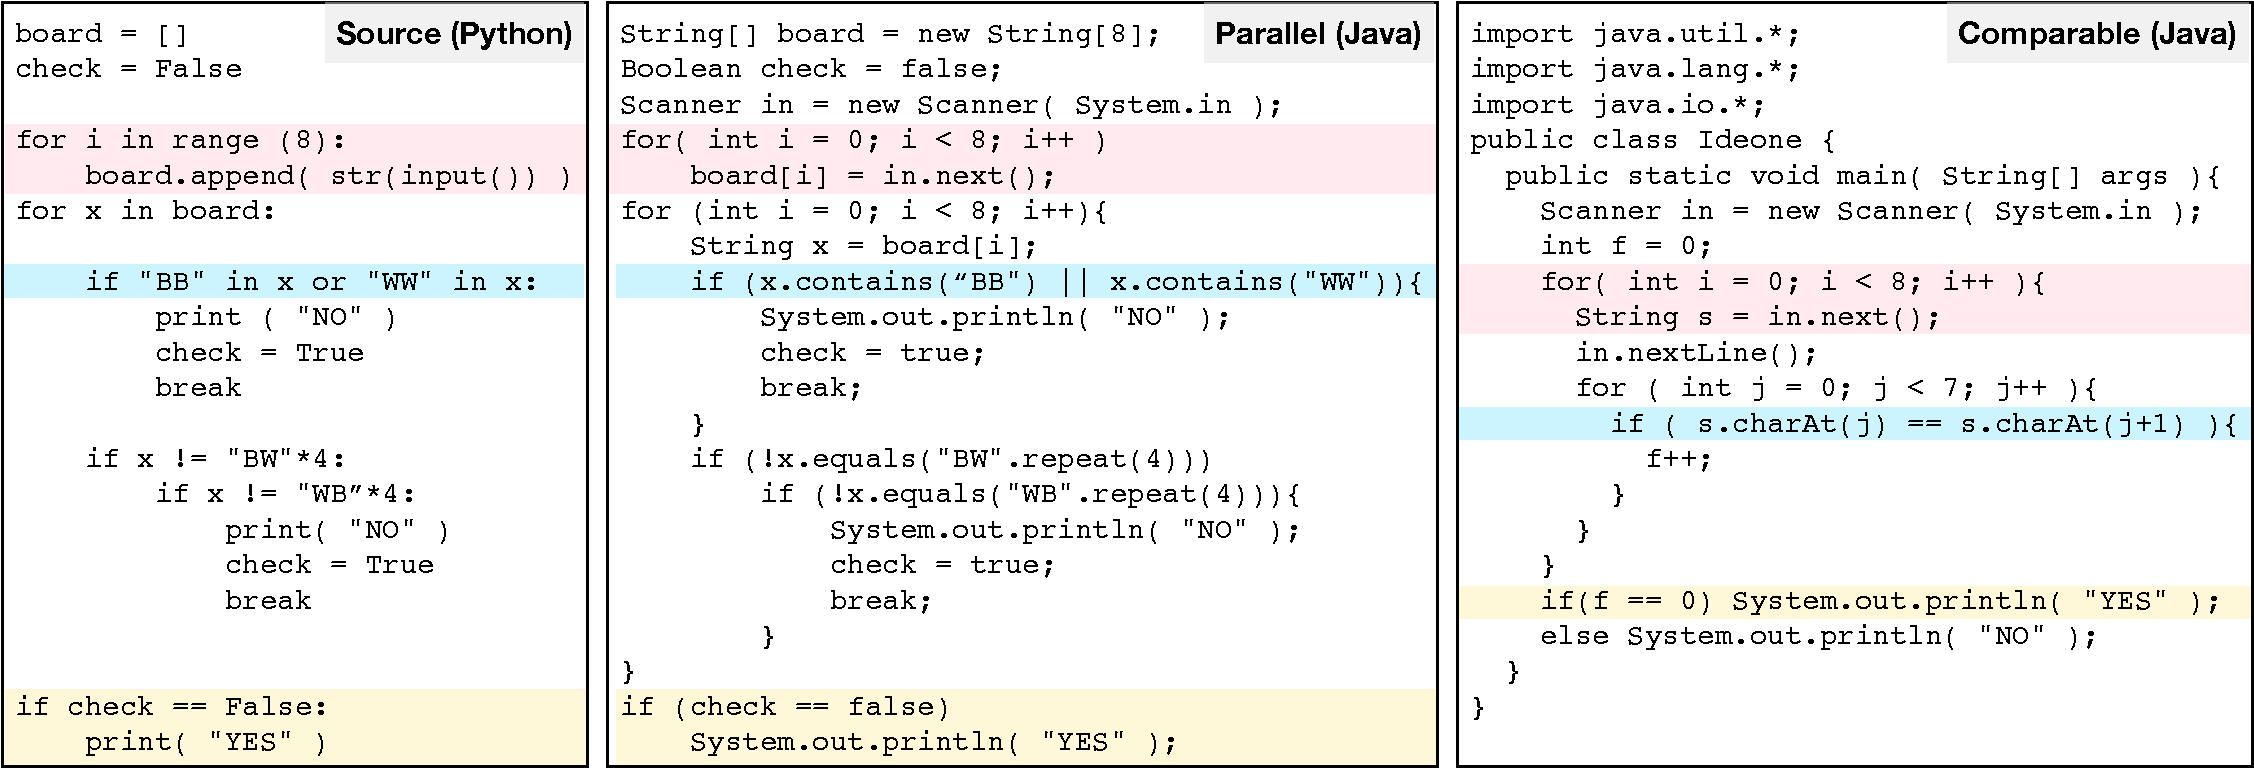
\includegraphics[width=\linewidth]{CMTrans_figs/examples_intro.pdf}
    \caption{An example of parallel and comparable data. Parallel examples are line-by-line aligned. Programs in a comparable example may have different algorithms and structures (e.g., global code vs. class in this case), but may still contain lines that can be matched, as highlighted in pink, blue, and yellow.}
    \label{fig:cmtrans_example_intro}
\end{figure}


\begin{figure}[t]
  \centering

  \begin{subfigure}[t]{0.4\linewidth}
    \centering
    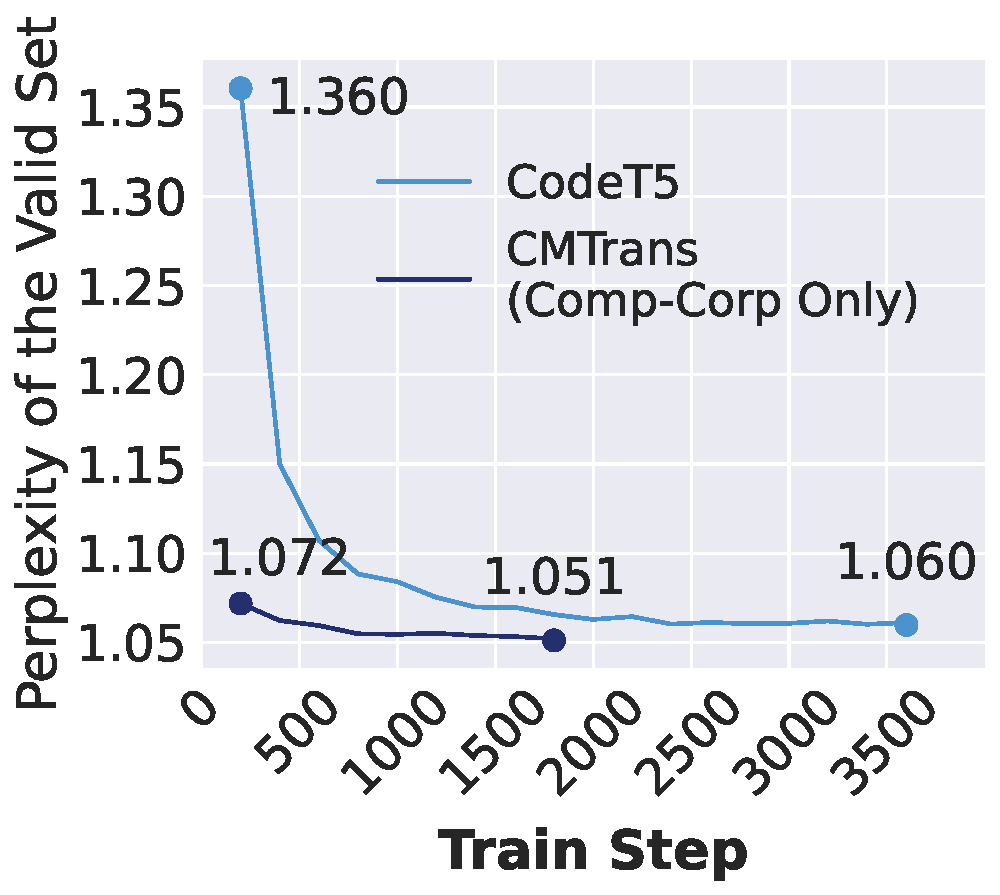
\includegraphics[width=\linewidth]{CMTrans_figs/ppl_java2python.pdf}
    \caption{Java-to-Python}
    \label{fig:cmtrans_ppl1}
  \end{subfigure}
  % \hfill%
  \begin{subfigure}[t]{0.4\linewidth}
    \centering
    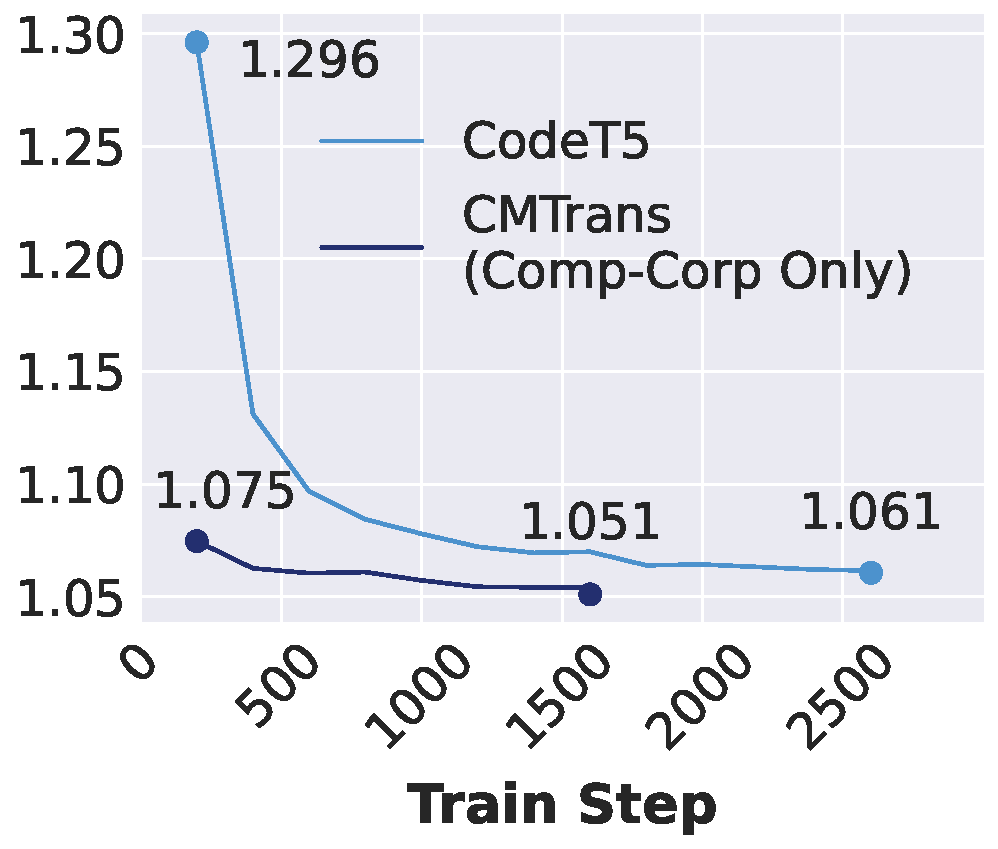
\includegraphics[width=\linewidth]{CMTrans_figs/ppl_python2java.pdf}
    \caption{Python-to-Java}
    \label{fig:cmtrans_ppl2}
  \end{subfigure}

  \caption{Perplexity of validation set during finetuning.}
  \label{fig:cmtrans_ppl}
\end{figure}


\section{Introduction}
In this chapter, we show a successful case of constructing scalable and effective training data for code translation.

% [motivate code translation]
Code translation is a special type of machine translation that translates between programming languages.
It is widely applied in software engineering to migrate a codebase into another programming language.
Recent code translation models typically follow the pretrain-finetune pipeline.
As shown in \autoref{fig:cmtrans_diagram_intro}, in pretraining, with denoising objectives such as masked span or identifier prediction \cite{plbart,codet5,transcoder}, the model learns to produce sequences in both languages.
When finetuned on parallel data \cite{avatar}, which are program pairs in the source and target language that are aligned line-by-line, the model learns functional equivalence: identifying programs with the same functionality,
either in the same language or between languages.
We show an example of parallel data in \autoref{fig:cmtrans_example_intro}.

One major challenge of code translation is that parallel data is typically limited. For instance, the TransCoder dataset \cite{transcoder} only contains 466 Python-C++ pairs. Constructing parallel data requires substantial human effort and cannot be easily scaled. 
With limited fine-tuning examples, it is difficult for a model to learn functional equivalence across programming styles and domains.

To mitigate the data scarcity issue, we pose three questions: \textbf{
(1) What does the model need to learn to perform code translation? 
(2) Does everything need to be learned from parallel data?
(3) If parallel data is still necessary, how to obtain parallel data in an efficient way?}

We answer the first question: what the model needs to learn, by comparing the model before and after finetuning. We observe that (1) the model learns to generate fluent code in the target language. As shown in \autoref{fig:cmtrans_ppl}, with the source language as input, before finetuning, the model continues to generate code in the source language, and the ground truth translation in the target language has a high perplexity.
(2) The model learns the functionality equivalence between the source and target languages. Namely, it learns the implementation of the same functionality in both languages. 

% [present the solution: comparable corpora of different types]
As for the second question, we show that both (1) and (2) can be learned from \emph{comparable corpora} to some extent, a term we borrow from natural language translation, where it refers to texts on similar topics in different languages \cite{NMTComparableCorpora,low_resource_comp_corpora}.
Here, we use it to refer to programs with similar functionality in different languages \cite{avatar,xcodeeval}.
As shown in \autoref{fig:cmtrans_example_intro}, although the programs paired in a comparable example may have different algorithms and structures (e.g., global code vs.\ class functions), they are likely to have similar constructs and may even have some lines that can be matched.

% [in this paper, the CC part]
In this paper, we \emph{study what the model learns from comparable corpora} by building three types of comparable examples:
(1) \emph{Naturally existing}, where we leverage independently-written solutions of the same coding problem;
(2) \emph{Generated}, where we collect programs with docstrings in one language and apply a code generation model to generate programs in another language; and
(3) \emph{Retrieved}, where we either retrieve a program's k nearest neighbors (KNN) or simply choose a random program in another language.
Among them, (1) contains cleaner examples, which are guaranteed to be bug-free. (3) covers programs from a larger variety of sources, providing more diverse training signals.

Since comparable corpora only contain program pairs with similar functionality, parallel data is still necessary to translate the precise functionality across different programming languages. 
As an answer to the third question, we notice that the majority of finetuning data only have one reference translation (e.g., 82.5\% in AVATAR, \citealt{avatar}).
However, code with different surface forms may have the same functionality (e.g., the interchange between \texttt{for loops} and \texttt{while loops}).
This makes it possible to augment the dataset by adding multiple reference translations with the same functionality, which reduces overfitting to a single translation and boosts the model to fully capture code semantics.

As a result, in this paper, we \emph{generate multiple translation references} for the finetuning data.
Specifically, after training on comparable corpora, we finetune a model on the original parallel data, generate multiple translations for each example, and use automatically generated test cases to filter out incorrect translations.
By training on different functionally equivalent programs, we reduce overfitting to a single output and improve the modeling of the target language.


% [results and analysis]
Combining the two techniques, we name our full approach \cmtransours, a code \textbf{Trans}lation model trained with \textbf{C}omparable corpora and \textbf{M}ultiple references.
Extensive experiments show that \cmtransours significantly improves CodeT5 \cite{codet5}, which is initialized from the same pretrained checkpoint, for an average of 7.5\% Computational Accuracy (CA@1) over translation between 6 language pairs.
\cmtransours also significantly outperforms the state-of-the-art method in 5 out of 6 language pairs, while reaching parity on the other one.

Analyses of our two techniques suggest that:
(1) All three types of comparable corpora (including random program pairs) improve the syntax accuracy and perplexity of the translation outputs and lead to better final performance.
(2) Both naturally existing and generated comparable corpora help the model generate constructs that match the input. The combination of them gives the largest performance gain.
(3) By training with multiple references, the model generates more unique correct translations within a certain budget, which indicates that better functional equivalence of the target language is learned.


% \section{Related Work}
% \start{Code Translation}
% Previous work has tackled the problem of translating code written in one programming language to another. 
% \citet{Karaivanov2014PhraseBasedST}, \citet{Nguyen2013LexicalSM,Nguyen2015DivideandConquerAF}, \citet{Phan2017StatisticalMO,Oda2015LearningTG} applied statistical machine translation techniques to code translation, while \citet{TreetotreeNN} introduced a tree-to-tree neural translation approach. 
% Further improvements were achieved by pre-trained language models of code such as CodeBERT \cite{codebert}, PLBART \cite{plbart}, and CodeT5 \cite{codet5}. 
% However, the above approaches require finetuning on parallel data, which is often scarce. 

% \start{Data Scarcity in Code Translation}
% To tackle the data scarcity issue, TransCoder \cite{transcoder} uses back translation for unsupervised code translation.
% DOBF \cite{dobf}, TransCoder-ST \cite{transcoderST}, and S\&G \cite{SandG} respectively improve TransCoder with de-obfuscation pre-training, self-training, and pairing up the model with a generation and a summarization model.
% However, the best-performing approach, TransCoder-ST, is only able to generate parallel data for standalone functions where the model can already generate a correct solution within a limited budget.
% In contrast, the comparable corpora we use to train \cmtransours include code with arbitrary structure and content.
% \cmtransours also has much better efficiency, as self-training requires running a much larger number of test cases than generating multiple references.
% MultiPL-E \cite{multiple} also automatically generates test cases, but retries until the output passes all test cases. We do not directly compare to it since it requires multiple rounds of translation.

% \start{Data Augmentation for Natural Language Translation}
% The lack of parallel training data is a fundamental problem in the field of translation, which has led the NLP community to develop several data augmentation techniques in response. 
% \textit{Comparable Corpora}, as defined by \citet{first_comp_corpora}, ``are texts that, while not parallel in the strict sense, are somewhat related and convey overlapping information''. 
% \citet{methods_collect_comp_corpora} and \citet{harvesting_comp_corpora} present methods for collecting comparable corpora to study when and how to use them. 
% \citet{handle_with_care_comp_corpora} and \citet{NMTComparableCorpora} identify information balance, alignment, and length differences between source and target as key factors affecting translation quality. 
% In this work, we extend the study of comparable corpora to code translation. 
% We show that code translation can benefit from multiple types of comparable corpora even if there is already high-quality parallel data. 
% We also provide analyses on why comparable corpora are beneficial.

% Another data augmentation strategy is using multiple translation references. 
% \citet{truly_exploring_multi_ref} and \citet{simulated_multi_ref} found that using multiple references can be beneficial in low-resource settings.
% An advantage of working with code is that test cases can be used to filter model-generated translated references to ensure functional equivalence to the source, which we exploit in \cmtransours.









\section{Methodology}
In this section, we introduce our data augmentation method that trains the model first on comparable corpora, which are either naturally existing, generated, or retrieved (\S\ref{sec:comparable}) and then on parallel data with additional references generated by \cmtransours (\S\ref{sec:multiref}).

\begin{figure}[t]
    \centering
    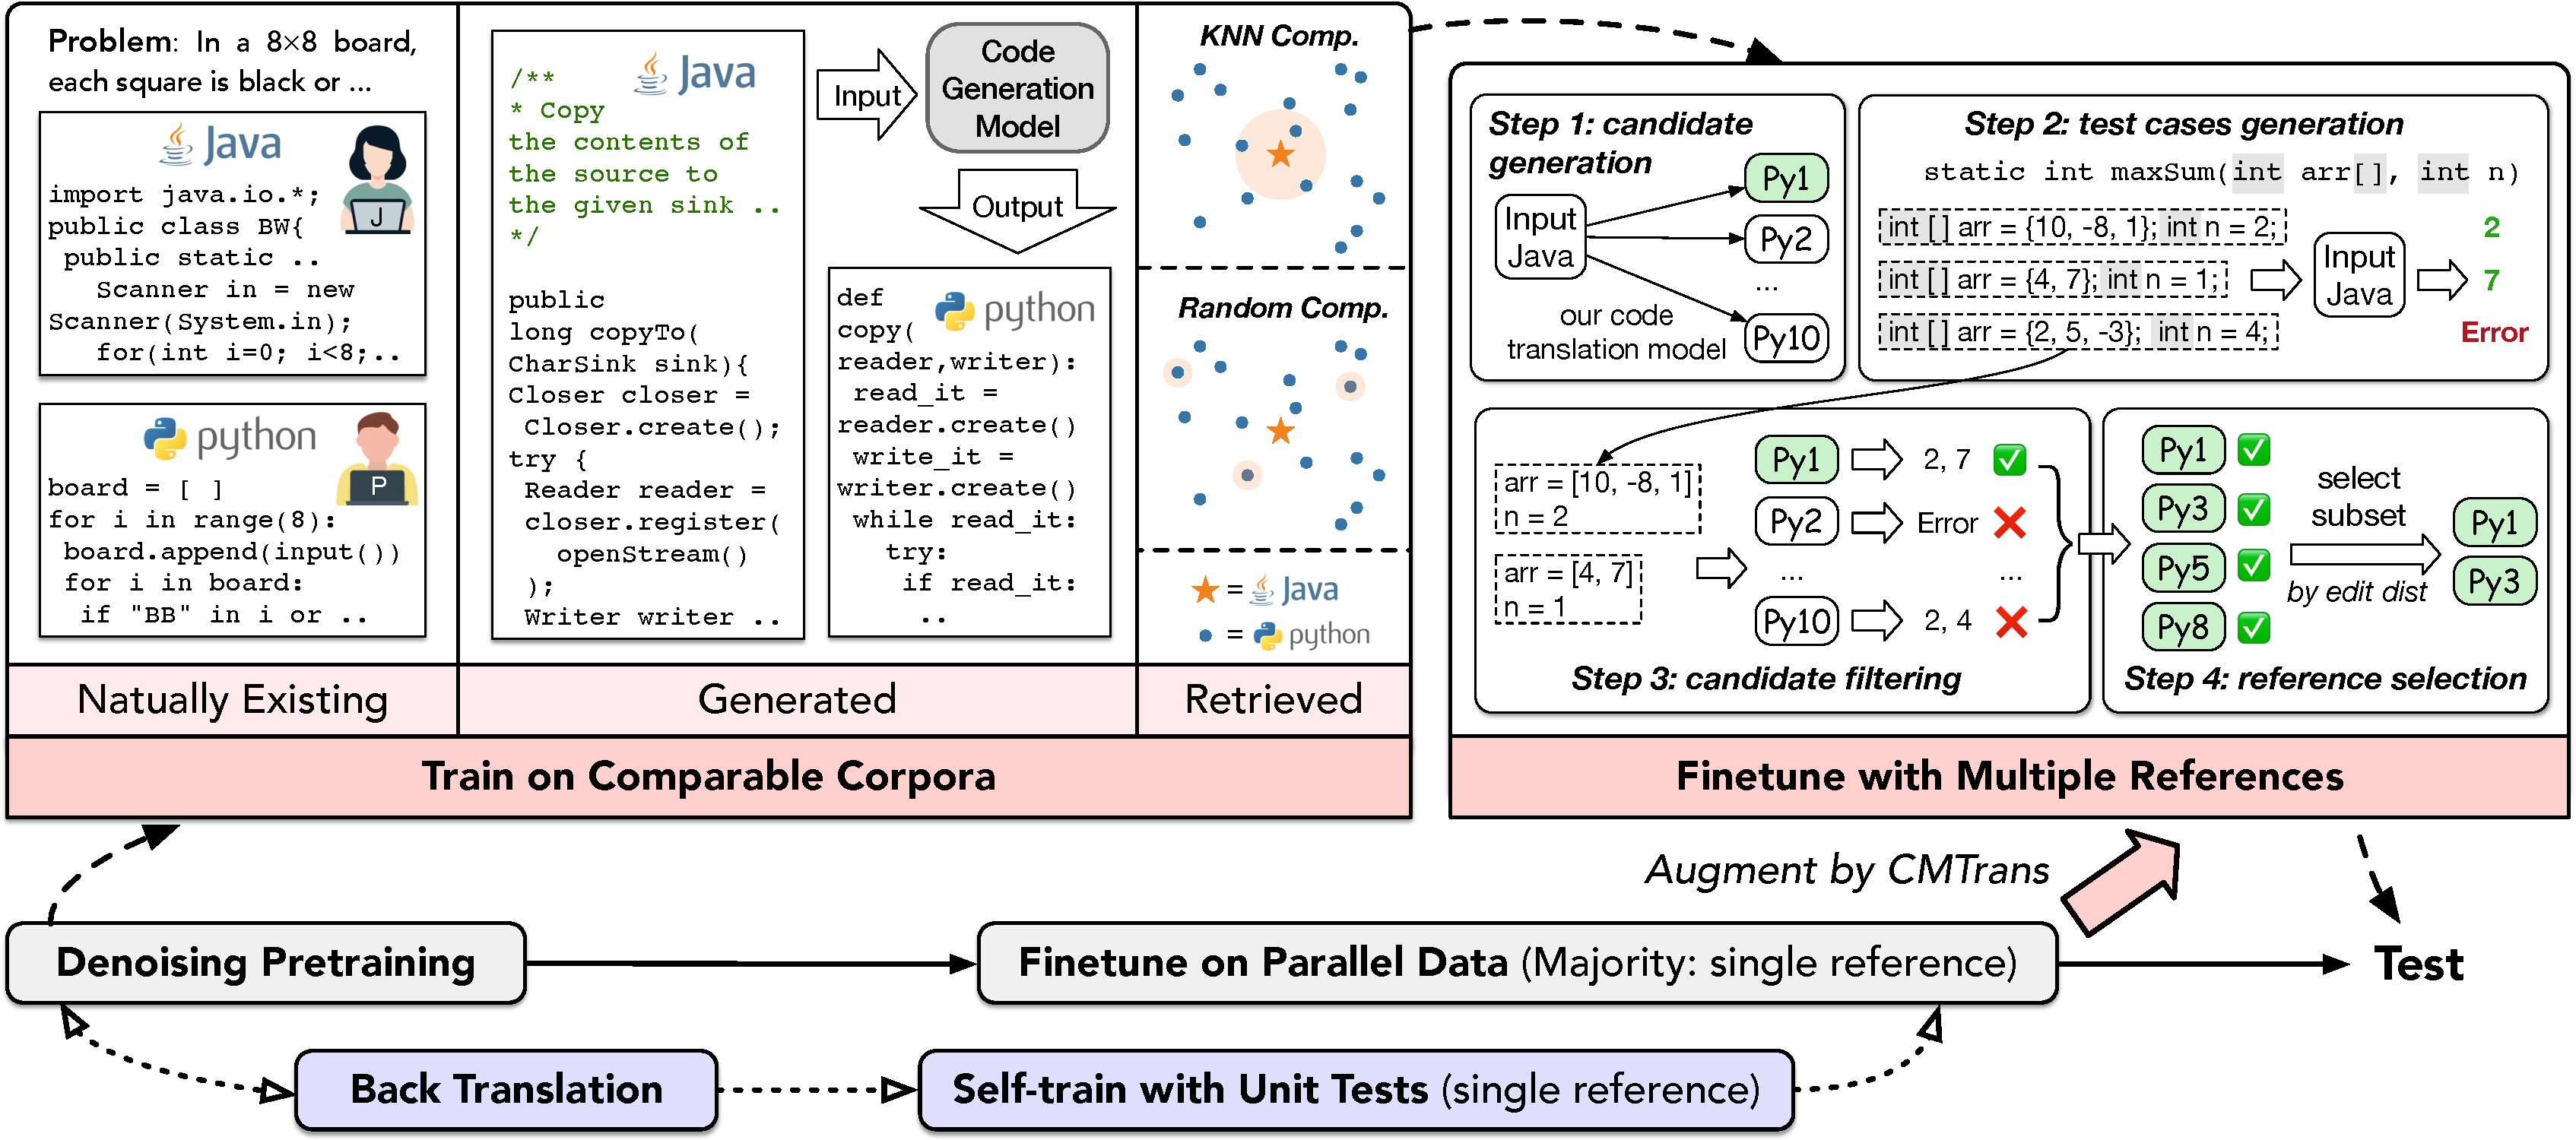
\includegraphics[width=\linewidth]{CMTrans_figs/method_v2.pdf}
    \upv
    \caption{An example of \cmtransours for Java-to-Python translation. We compare the pipeline of \cmtransours (\textit{red}) to the standard pipeline (\textit{grey}) of code translation (e.g., finetuned CodeT5, \citealt{codet5}) and the self-supervision-and-fine-tuning method (\textit{purple}) of TransCoder-ST (\citealt{transcoderST}).}
    \label{fig:cmtrans_method}
    \downv
\end{figure}

\subsection{Problem Formulation}
We formulate code translation as a sequence-to-sequence (Seq2Seq) generation problem following existing work \cite{codexglue,avatar,transcoder}.
The input is the code in the source language $S = \{s_1, s_2, ..., s_n \}$, which is a sequence of tokens.
We apply a model to translate the input code into the target language $T = \mathcal{M}_{\theta}(S) = \{t_1, t_2, ..., t_m \}$, where the model $\mathcal{M}_{\theta}$ is typically finetuned for code translation. 
Alternatively, the model may generate $k$ candidate outputs for each input: $\mathcal{M}_{\theta}(S,k) = \mathbb{T} = \{ T^{(1)}, T^{(2)}, ..., T^{(k)} \}$. 

\subsection{Training on Comparable Corpora}
\label{sec:comparable}

As shown in \autoref{fig:cmtrans_method}, we study three types of comparable corpora: naturally existing, generated, and retrieved ones. Here we introduce how we build each type of comparable examples and train \cmtransours on them.

\start{Naturally Existing Comparable Examples}
We make use of comparable corpora collected from programming contests by existing datasets \cite{avatar,xcodeeval,codenet}, which mainly consist of solutions to the same contest problems written in different languages.
These comparable examples are typically confined to specific domains such as dynamic programming or graph theory.


\start{Generated Comparable Examples}
To cover programs in more diverse domains, we present a method that automatically generates comparable examples using natural-language-to-code generation models.

Specifically, we leverage a monolingual corpus of functions with natural language documentation (i.e., docstrings) to describe their functionality.
In the experiments, we use GitHub functions with docstrings extracted by CodeSearchNet \cite{codesearchnet}.
For each function $S_c$ in the corpus, we feed the natural language documentation to a code generation model finetuned in the other language, which is trained to generate a program based on the given natural language description.
Similarly to code translation, the code generation model can generate multiple candidate outputs $\{ T_c^{(1)}, T_c^{(2)}, ..., T_c^{(k)} \}$.
We then select the one with the highest probability, which is paired up with the extracted program as a comparable example.


\start{Retrieved Comparable Examples}
To study the effect of the quality of comparable corpora, we further build \textbf{KNN Comparable Corpora}.
We compute the embedding of all the programs in the source and target language in the dataset using a finetuned code retrieval model~\cite{codesearchnet}.
For each program $S$ in the source language with embedding $emb(S)$, we retrieve its k nearest neighbors in the target language by the cosine similarity between their embeddings: $sim(S,T) = \langle emb(S), emb(T) \rangle$.

Finally, we build \textbf{Random Comparable Corpora} by pairing random programs in the source and target language.
In principle, such program pairs do not contain any information on functional equivalence and allow us to better understand whether comparable corpora can improve the modeling of the target language and hence improve the translation quality.



\start{Model Training}
After constructing a corpus of comparable examples $\mathcal{D}_c = \{(S_c, T_c)\}$, we input the program in the source language $S_c$ into \cmtransours $\mathcal{M}_{\theta}$ and maximize the log-likelihood of its corresponding program in the target language $T_c = \{t_{c,1}, t_{c,2}, ..., t_{c,m} \}$:
\begin{align}
\begin{split}
&\mathcal{L}_{M T}(\mathcal{D}_c) = \sum_{(S_c, T_c) \in \mathcal{D}_c} P_{\theta}(T_c | S_c) \\
&P_{\theta}(T_c | S_c) = -\sum_i \log \left(P_{\theta}\left(t_{c,i} | S_c, t_{c,1} \ldots t_{c,i-1} \right)\right)
\end{split}
\label{eq:mtloss}
\end{align}

Here $\theta$ is the parameter of $\mathcal{M}_{\theta}$, which is initialized from an encoder-decoder model pretrained on code \cite{codet5}.
After training the model on the corpus comparable examples $\mathcal{D}_c$ till convergence, we finetune it on the dataset of parallel examples $\mathcal{D}_p$, where the loss $\mathcal{L}_{M T}(\mathcal{D}_p)$ is computed by \autoref{eq:mtloss} as well.

By maximizing the probability of the target $T_c$, the model will learn to generate fluent code in the target language.
Furthermore, in general, programs in a comparable example often exhibit the same types of constructs.
In the examples in \autoref{fig:cmtrans_example_intro}, to check whether a board is valid, no matter what algorithm is used, the program will always need a loop to read the board and use if statements for the validity check.
As a result, in principle, the model can also learn to generate the same types of constructs as the input program $S_c$, which is beneficial for generating accurate translations.


\subsection{Finetuning with Multiple References}
\label{sec:multiref}
In addition to comparable corpora, we also provide \cmtransours with more diverse training signals by finetuning with multiple references. 
By providing the model with programs with the same functionality, we encourage the model to learn a better representation space for the target language and hence benefit the translation.

Since the majority of source programs only have one reference in existing datasets of parallel examples \cite{avatar}, we apply a series of steps to generate additional references, which are illustrated in \autoref{fig:cmtrans_method}.
The first step is to finetune a model with the original parallel data, and then use the finetuned model to generate multiple translation candidates $\{ T_c^{(1)}, T_c^{(2)}, ..., T_c^{(k)} \}$ for each source program in the parallel data.

In the second and third steps, similar to TransCoder-ST \cite{transcoderST}, we leverage automatically generated unit tests to filter out candidates with different behaviors as the source program.
Specifically, we extract the input arguments of the source programs, randomly produce a set of test inputs based on the argument types, and feed the test inputs to the source program.
We filter out test inputs that cause compilation or runtime errors.
Finally, we feed the remaining test inputs to each candidate and only keep the ones that have exactly the same output as the source program.

Notice that some of the translations may only have small differences (e.g., \texttt{i++} vs. \texttt{i+=1}). To obtain a diverse subset of references, we select the most distinct $k$ translations for each source program by their string edit distance.
These $k$ translations are added as additional references to the finetuning set.




\begin{table}[t]
\centering
\resizebox{\textwidth}{!}{
\begin{tabular}{lcccc|c}
\toprule
\multirow{2}{*}{\bf Dataset $\rightarrow$}
& \multicolumn{3}{c}{\textbf{Train (Comparable)}} & \textbf{Train (Parallel)} & \textbf{Test} \\ 
\cmidrule(lr){2-4}  \cmidrule(lr){5-5} \cmidrule(lr){6-6}
& \textbf{Gen-comp} & \textbf{XCodeEval} & \textbf{AVATAR-comp} 
& \textbf{AVATAR-para} & \textbf{TransCoder-test} \\
\midrule
\bf \# C++ $\leftrightarrow$ Java & 4,053* & 3,414 & -- & 3,226* & 482 C-to-J, 467 J-to-C \\
\bf \# C++ $\leftrightarrow$ Python & 4,053* & 4,376 & -- & 3,226* & 464 C-to-P, 467 P-to-C \\
\bf \# Java $\leftrightarrow$ Python & 22,181* & -- & 5,937 & 3,391 & 464 J-to-P, 482 P-to-J \\ 
\bf Source 
& \begin{tabular}[c]{@{}c@{}}
Github (Java $\leftrightarrow$ Python) \\
AIZU, AtCoder (Others)
\end{tabular}
& Codeforces 
& \begin{tabular}[c]{@{}c@{}} 
AtCoder, Codeforces, ProjectEuler, \\ 
CodeJam, GeeksforGeeks, LeetCode, 
\end{tabular} 
& GeeksforGeeks 
& GeeksforGeeks \\
\bottomrule
\end{tabular}
}
\caption{Number of problems per dataset. ``Gen-comp'' is the comparable corpora dataset we generate. C-to-J, C-to-P, ... denote the test examples of C++-to-Java, C++-to-Python translation, etc. * denotes data we build.}
\label{tab:cmtrans_dataset}
\end{table}







\section{Results}

\begin{table}[t]
\centering
\resizebox{0.8\textwidth}{!}{
\begin{tabular}{lccccccccc}
\toprule
\multirow{2}{*}{\bf Model $\downarrow$}
& \multicolumn{3}{c}{\bf Java-to-Python} 
& \multicolumn{3}{c}{\bf Python-to-Java} 
& \multicolumn{3}{c}{\bf Avg of 6 Pairs} 
\\
% \midrule
\cmidrule(lr){2-4}  \cmidrule(lr){5-7} \cmidrule(lr){8-10}
% \bf Model $\downarrow$
& \bf BLEU & \bf CB & \bf CA@1 
& \bf BLEU & \bf CB & \bf CA@1 
& \bf BLEU & \bf CB & \bf CA@1 \\
\midrule
TransCoder \cite{transcoder} & 72.4 & 67.9 & 49.1 & 65.4 & 70.7 & 35.7 
& 72.0 & 75.0 & 51.7 \\
DOBF \cite{dobf} & 72.2 & 67.5 & 52.2 & 67.7 & 71.2 & 44.4 
& --- & --- & --- \\
TransCoder-ST \cite{transcoderST} & 73.1 & 68.7 & 68.5 & 70.0 & 71.9 & 58.1 
& 71.3 & 74.9 & 66.3 \\
\midrule
CodeBERT \cite{codebert} & 52.0 & 48.9 & 10.4 & 45.4 & 45.0 & 4.2 
& --- & --- & --- \\
CodeT5 \cite{codet5} & 79.4 & 72.5 & 61.0 & 79.0 & 75.9 & 52.7 
& \underline{83.6} & 80.0 & 62.6 \\
PLBART \cite{plbart} & \underline{79.9} & \underline{73.2} & 68.9 & 80.5 & 76.8 & 57.5 
& --- & --- & --- \\
TransCoder-ST-ft \cite{transcoderST} & 79.3 & 72.9 & \underline{69.4} & \underline{81.4} & \underline{78.4} & \underline{62.0} 
& 81.8 & \underline{80.2} & \underline{67.6} \\
\midrule
\cmtransours & \bf 80.1 & \bf 74.2 & \bf 73.5 & \bf 84.3 & \bf 82.1 & \bf 66.0 
& \bf 84.9 & \bf 82.0 & \bf 70.1 \\ 
\bottomrule
\end{tabular}
}
\caption{Java-Python translation results on TransCoder-test. We copy the results of all the baselines reported by \citet{avatar}. 
CB and CA@1 stand for CodeBLEU and Computational Accuracy. 
We highlight the \textbf{best} results under each metric with Bold and underline the \underline{second-best} results.}
\label{tab:cmtrans_main}
\end{table}

\begin{table}[t]
\centering
\resizebox{\textwidth}{!}{
\begin{tabular}{lcccccccccccc}
\toprule
\multirow{2}{*}{\bf Model $\downarrow$}
% \midrule
& \multicolumn{3}{c}{\bf C++-to-Java} 
& \multicolumn{3}{c}{\bf C++-to-Python}
& \multicolumn{3}{c}{\bf Java-to-C++} 
& \multicolumn{3}{c}{\bf Python-to-C++} \\
% \midrule
\cmidrule(lr){2-4}  \cmidrule(lr){5-7} \cmidrule(lr){8-10} \cmidrule(lr){11-13}
& \bf BLEU & \bf CB & \bf CA@1 
& \bf BLEU & \bf CB & \bf CA@1 
& \bf BLEU & \bf CB & \bf CA@1 
& \bf BLEU & \bf CB & \bf CA@1 \\
\midrule
TransCoder \cite{transcoder} & 84.0 & 86.7 & 65.1 & 75.2 & 73.4 & 47.1 & 83.6 & 85.4 & 79.8 & 51.6 & 65.7 & 32.6 \\
TransCoder-ST \cite{transcoderST} & 78.8 & 85.2 & 68.0 & 73.1 & 73.0 & 61.3 & 76.7 & 83.7 & \bf 84.6 & 55.8 & 67.1 & 56.7 \\
\midrule
CodeT5 \cite{codet5} & \underline{90.9} & 90.0 & 65.1 & \underline{82.9} & \underline{75.4} & 56.5 & 89.1 & \bf 88.5 & 81.6 & \underline{79.8} & \underline{77.9} & 58.5 \\
TransCoder-ST-ft \cite{transcoderST} & 88.7 & \underline{90.1} & \underline{68.3} & 75.4 & 74.3 & \underline{62.5} & \underline{89.3} & 87.8 & \bf 84.6 & 76.7 & 77.6 & \underline{59.1} \\
\midrule
\cmtransours & \bf 91.6 & \bf 90.5 & \bf 71.4 & \bf 83.7 & \bf 77.2 & \bf 64.2 & \bf 89.7 & \underline{88.4} & \underline{84.4} & \bf 82.0 & \bf 79.3 & \bf 61.2 \\
\bottomrule
\end{tabular}
}
\caption{Java-C++ and Python-C++ translation results on TransCoder-test. The CA@1 results of TransCoder and TransCoder-ST are copied from the TransCoder-ST paper. We evaluate BLEU and CodeBLEU using their released checkpoints. We finetune and evaluate CodeT5 and TransCoder-ST-ft on our own.}
\label{tab:cmtrans_cpp}
\end{table}


In this section, we conduct experiments to answer four
research questions: 
(\textbf{RQ1}) How do \cmtransours and its ablations perform compared against state-of-the-art approaches for code translation?
(\textbf{RQ2}) What can the model learn from comparable corpora?
(\textbf{RQ3}) What can the model learn from multiple references? 
(\textbf{RQ4}) How is \cmtransours affected by the size of comparable corpora and the number of references?

\subsection{Experimental Setup}
\label{sec:setup}
We initialize \cmtransours from the pretrained checkpoint of CodeT5 \cite{codet5}, an encoder-decoder model pretrained on code files from varied languages with denoising objectives.

\start{Datasets}
We list the dataset statistics in \autoref{tab:cmtrans_dataset}.
All the methods are evaluated on the TransCoder-test dataset~\cite{transcoder}.
We train our method on xCodeEval \cite{xcodeeval}, a comparable corpora dataset, and AVATAR \cite{avatar}, which contain both comparable corpora and parallel functions (denoted as AVATAR-comp and AVATAR-para, respectively).
All the supervised baseline methods are finetuned on AVATAR-para before evaluation.

Since AVATAR-para does not contain C++ functions, we add a parallel C++ function for each training example in AVATAR-para. Specifically, we generate 50 C++ translations for each Java function by TransCoder-ST, TransCoder, and finetuned CodeT5 and filter the translations with unit tests.

\start{Construction of Comparable Corpora}
We conduct the study on different types of comparable corpora (\CC) on Java $\leftrightarrow$ Python translation.
We use AVATAR-comp\footnote{There are two versions of AVATAR-comp with slight differences. We use the first version because most of our experiments were finished before the second version was released.} as the naturally existing \CC.
KNN and random \CC are also retrieved from AVATAR-comp.
To build the dataset of generated \CC (denoted as Gen-Comp), we generate from functions with docstrings in the CodeSearchNet~\cite{codesearchnet} dataset.

We train \cmtransours first on the best combination of comparable corpora, which is natural and generated \CC, and then finetuned on AVATAR-para.
For language pairs other than Java $\leftrightarrow$ Python, we use xCodeEval as naturally existing \CC and generate \CC from CodeNet~\cite{codenet}. 
% More details can be found in Appendix~\ref{sec:implementation}.


\start{Evaluation metrics}
Our primary metric is the Computational Accuracy (CA@k), which evaluates whether at least 1 out of k translation candidates generates the same outputs as the reference for all the given test inputs.
Following previous work \cite{avatar}, we report \textbf{CA@1} results and also report \textbf{BLEU}, which computes the overlap between candidate and reference translations \cite{BLEU}, and \textbf{CodeBLEU}: the weighted average of token level match, syntax level match, and Dataflow match \cite{codebleu}.
% Appendix \ref{sec:implementation} contains more details about the implementation and baselines.


\subsection{Main results}
\autoref{tab:cmtrans_main} and \autoref{tab:cmtrans_cpp} show the code translation results on TransCoder-test.

\cmtransours substantially outperforms CodeT5, which is initialized from the same pretrained checkpoint and finetuned with the original parallel data, by an average improvement of 7.5\% CA@1.
\cmtransours also significantly outperforms the state-of-the-art methods, TransCoder-ST-ft, on 5 out of 6 language pairs, and reaches parity on Java-to-C++ translation.
Note that TransCoder-ST-ft generates test cases for 103,488 functions and executes these test cases over 4 iterations of training. 
In comparison, \cmtransours only generates test cases for 3,391 functions and executes the test cases once, resulting in better efficiency.

Our results show that the advantage of \cmtransours is larger on translations between Java and Python. The reason may be that the parallel data we generate for translations involving C++ are only verified by automatically generated test cases, which might not cover all the boundary cases and could introduce noise to the finetuning set.
Following previous work~\cite{transcoderST,avatar}, we report the results of one checkpoint. 
% We also conduct the t-test in Appendix~\ref{sec:ttest}, which indicates that \cmtransours significantly outperforms the best baseline over CA@1 with p-value $<$ 0.01 for 4 out of 6 language pairs and with p-value $<$ 0.05 for one language pair.

\subsection{Performance Analysis}
\start{Ablation studies}
\autoref{tab:cmtrans_ablation} presents the ablations of our approach. 
We first study the effectiveness of each type of comparable corpora and some combinations of them. All the ``+ \CC'' ablations denote training CodeT5 on comparable corpora and then finetuneing on AVATAR-para.
We also ablate ``+ Multi-Ref'', which is finetuned on multiple references directly after pretraining.
The results show that both Multi-Ref and the best \CC provide a large performance gain and stacking them (the full \cmtransours) has the best performance.

As for the effectiveness of different \CC, we can see that code translation can benefit from all these types of \CC. The combination of Natural and generated \CC has the best performance. The reason might be both \CC have relatively high data quality and further adding the other two \CC in training introduces noise to the model and hinders the learning of functional equivalence.

Notice that with the same finetuning set, \textit{\CC\ Only} still outperforms TransCoder-ST-ft, which indicates that compared to self-training, training on comparable corpora has not only better efficiency but better effectiveness.
We hypothesize that the reason may be that the comparable corpora contain more diverse structures and contents. This provides more diverse training signals to the model and hence improves the generalization.

\begin{table}[t]
\centering
\resizebox{0.6\linewidth}{!}{
\begin{tabular}{lcc}
\toprule
% \midrule
\bf Model $\downarrow$ & \bf J-to-P CA@1 & \bf P-to-J CA@1 \\
\midrule
CodeT5 & 61.0 & 52.0 \\
+ Random \CC & 64.7 & 54.6 \\
+ KNN \CC & 63.8 & 55.4 \\
+ Generated \CC & 64.0 & 63.1 \\
+ Natural \CC & 68.8 & 62.9 \\ 
\midrule
+ All \CC & 62.5 & 55.4 \\
+ Natural \& Generated & 70.0 & 64.1 \\ 
+ Multi-Ref & 68.1 & 61.6 \\ 
\cmtransours & \bf 73.5 & \bf 66.0 \\ 
\bottomrule
\end{tabular}
}
\caption{Ablation studies of \cmtransours. We report CA@1 results. J-to-P and P-to-J stand for Java-to-Python and Python-to-Java results. We put the experiments on each type of comparable corpora in an individual block.}
\label{tab:cmtrans_ablation}
\end{table}



\start{Translation with Limited Parallel Data}
To analyze how well \cmtransours tackles the data scarcity challenge, we compare the performance of CodeT5 and \cmtransours when finetuned on parallel data with different sizes.
For simplicity, we use \cmtransours (\CC Only) to denote the ``CodeT5 + Natural \& Generated'' ablation 
and use \cmtransours (Multi-Ref\ Only) to denote ``CodeT5 + Multi-Ref''.

As shown in \autoref{fig:cmtrans_size}, the relative gains of \cmtransours as well as our ablations are more pronounced when the parallel data is more limited. 
For example, when there are only 100 parallel examples for Java-to-Python translation, CodeT5 obtains 6.5 CA@1 while \cmtransours, (\CC Only), and (Multi-Ref\ Only) obtain 43.1, 39.7, and 26.9 CA@1, respectively. 
This demonstrates the effectiveness of our two data augmentation techniques to tackle data scarcity.

\begin{figure}[t]
    \centering
    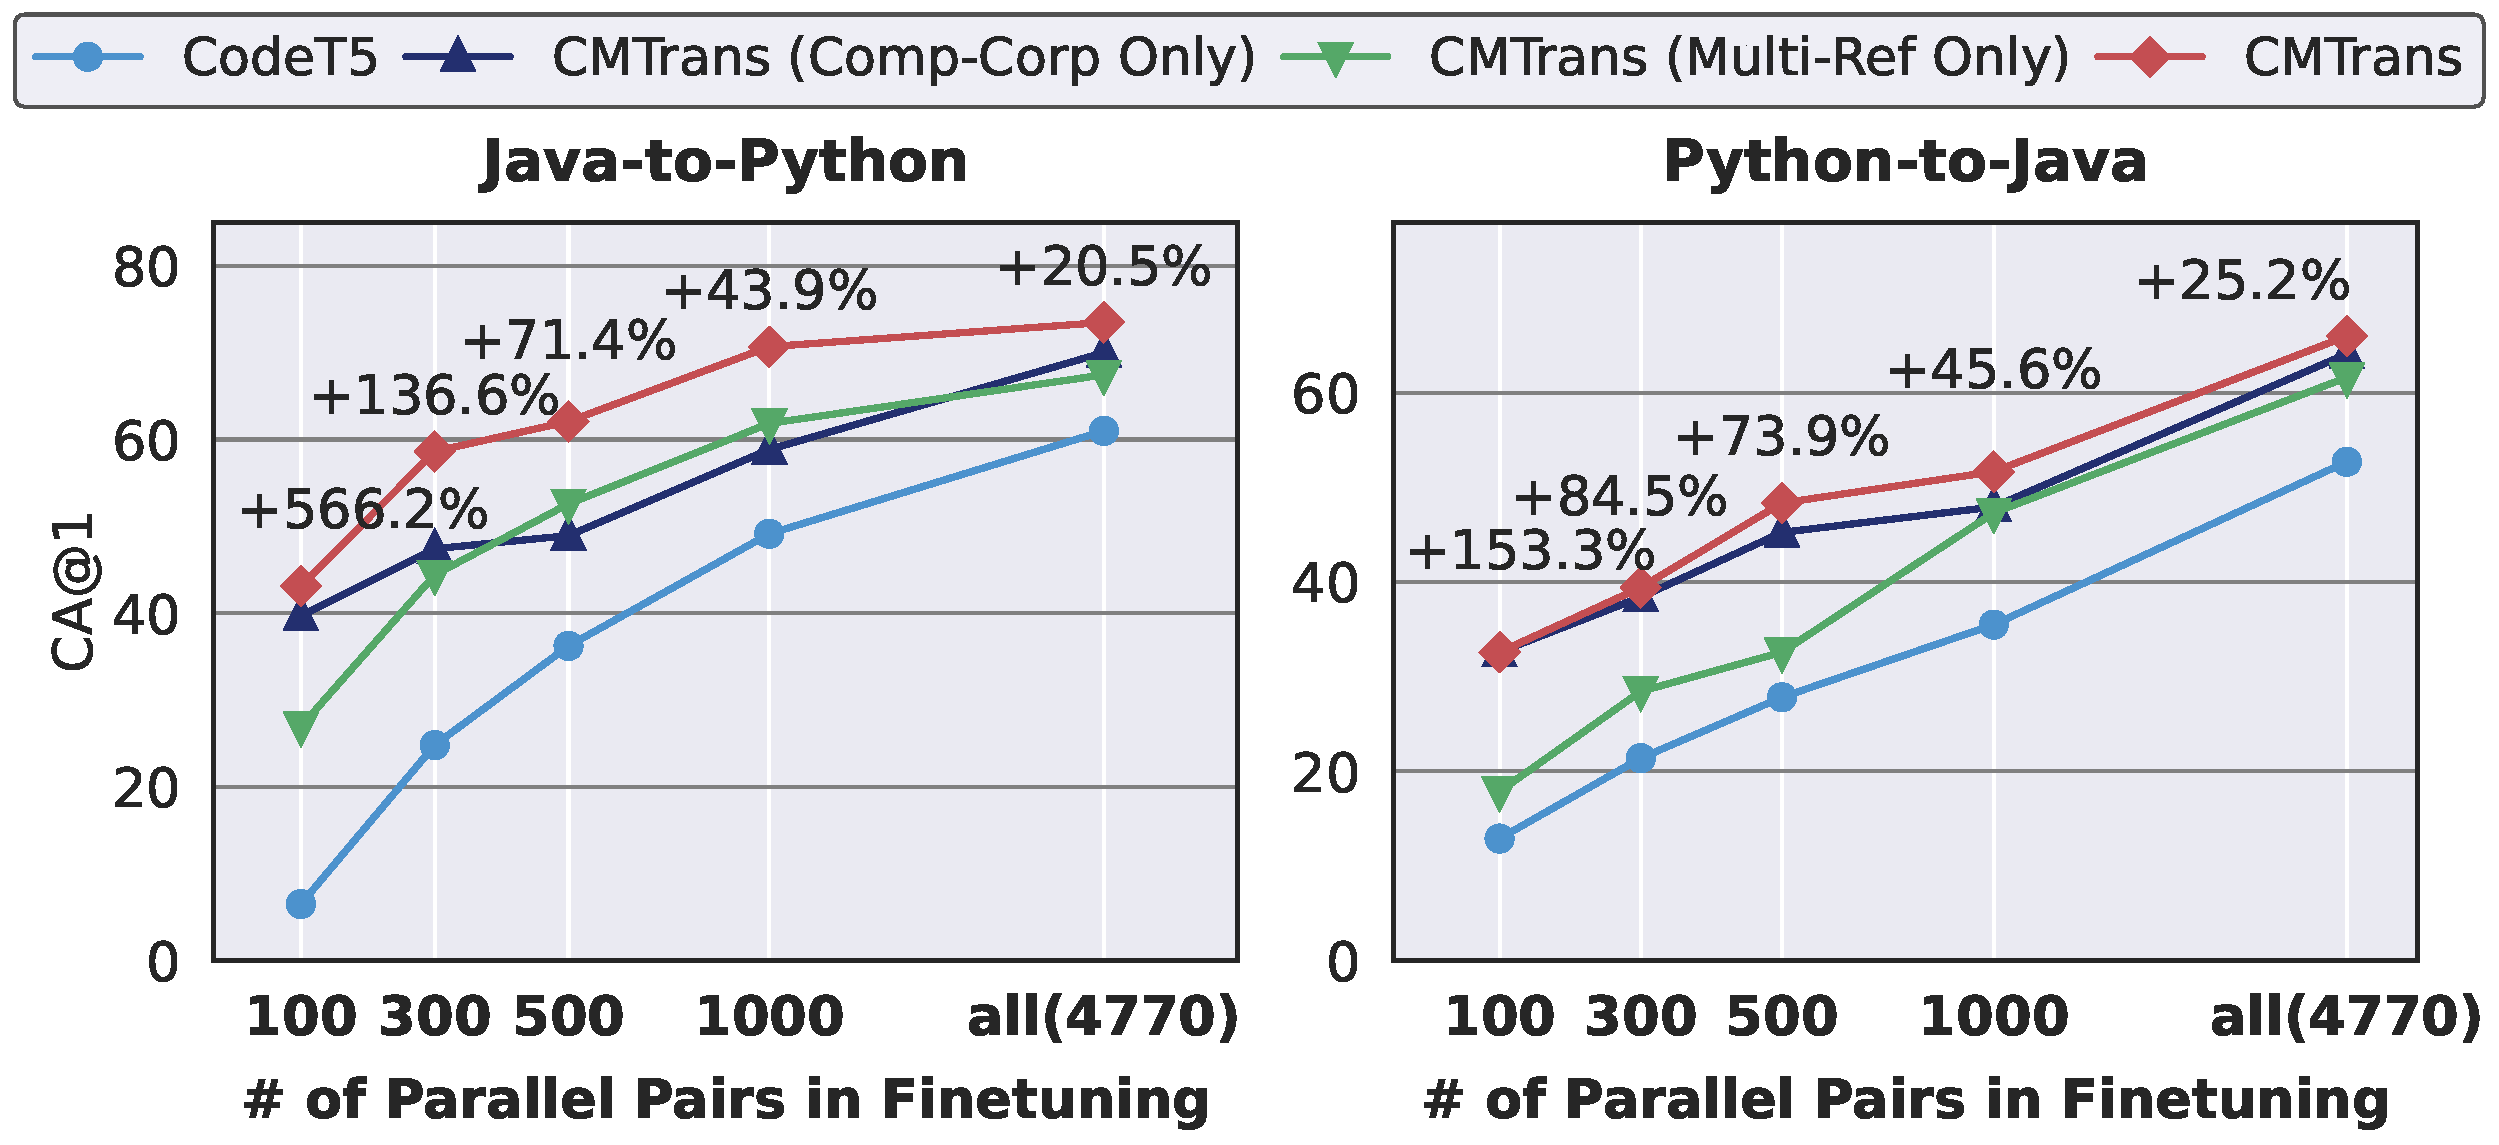
\includegraphics[width=0.7\linewidth]{CMTrans_figs/size_analysis_fig.pdf}
    \caption{Translation results with different amount of parallel data. We mark the relative gain of \cmtransours over CodeT5.}
    \label{fig:cmtrans_size}
\end{figure}

\begin{table}[t]
\centering
\resizebox{\linewidth}{!}{
\begin{tabular}{lccccccccc|ccccccccc}
\toprule
\multirow{3}{*}{\bf Model $\downarrow$}
& \multicolumn{9}{c}{\bf Java-to-Python} 
& \multicolumn{9}{c}{\bf Python-to-Java} \\
\cmidrule(lr){2-10} \cmidrule(lr){11-19} 
& \multicolumn{3}{c}{\bf LOOP} 
& \multicolumn{3}{c}{\bf IF} & \multicolumn{3}{c}{\bf ELSE IF} 
& \multicolumn{3}{c}{\bf LOOP} 
& \multicolumn{3}{c}{\bf IF} & \multicolumn{3}{c}{\bf ELSE IF} \\
\cmidrule(lr){2-4}  \cmidrule(lr){5-7} \cmidrule(lr){8-10}
\cmidrule(lr){11-13}  \cmidrule(lr){14-16} \cmidrule(lr){17-19}
& P & R & F1 & P & R & F1 & P & R & F1 
& P & R & F1 & P & R & F1 & P & R & F1 \\
 \midrule
CodeT5 (No finetune) & 100.0 & 28.5 & 44.4 & 99.1 & 35.4 & 52.2 & 0.0 & 0.0 & 0.0 &
100.0 & 14.6 & 25.5 & 100.0 & 36.6 & 53.6 & 0.0 & 0.0 & 0.0 \\
+ KNN \CC & 89.4 & 94.6 & 91.9 & 82.1 & 64.3 & 72.1 & 41.6 & 57.6 & 48.3 & 
87.9 & 98.9 & 93.1 & 90.2 & 50.9 & 65.1 & 30.5 & 16.4 & 21.3 \\
+ Generated \CC & 99.9 & 98.9 & \bf 99.4 & 99.0 & 93.2 & \bf 96.0 & 84.6 & 79.2 & \bf 81.8 & 98.3 & 96.7 & \bf 97.5 & 98.7 & 94.8 & \bf 96.7 & 83.3 & 86.4 & \bf 84.8 \\
+ Natural \CC & 95.8 & 85.4 & 90.3 & 91.2 & 73.9 & 81.6 & 50.0 & 49.6 & 49.8 & 87.4 & 98.9 & 92.8 & 88.2 & 80.4 & 84.1 & 57.8 & 33.6 & 42.5 \\
\bottomrule
\end{tabular}
}
\caption{The overlap between the types of constructs in the translation outputs and the ground truth translations. }
\label{tab:cmtrans_construct}
\end{table}


\begin{table}[t]
\centering
\resizebox{0.6\linewidth}{!}{
\begin{tabular}{lcc}
\toprule
\bf Model $\downarrow$ & \bf J-to-P SA& \bf P-to-J SA \\
\toprule
No finetuning on parallel pairs \\
\midrule
CodeT5 \cite{codet5} & 1.1 & 1.7 \\
+ Random \CC & 20.0 & 41.3 \\
+ KNN \CC & 22.0 & \bf 56.4 \\
+ Generated \CC & \bf 41.4 & 43.2 \\
+ Natural \CC & 34.1 & 54.6 \\
\toprule
With finetuning on parallel pairs \\
\midrule
CodeT5 \cite{codet5} & 95.3 & 69.7 \\
+ Random \CC & 96.3 & 69.7 \\
+ KNN \CC & 96.3 & 71.0 \\
+ Generated \CC & \bf 97.6 & 71.2 \\
+ Natural \CC & 97.4 & \bf 76.4 \\
\bottomrule
\end{tabular}
}
\caption{Syntax Accuracy (SA) on TransCoder-test before finetuning, which evaluates whether the program can be compiled without syntax errors.}
\label{tab:cmtrans_EA}
\end{table}



\subsection{Influence of Comparable Corpora}
To answer \textbf{RQ2}, we hypothesize that training on comparable corpora allows the model to produce fluent code in the target language while using similar constructs as the input.


\start{Fluency of outputs}
To validate our hypothesis, we compare the perplexity of the reference translations (in the target language) during finetuning, which reflects the fluency of outputs.
As shown in \autoref{fig:cmtrans_ppl}, after training on comparable corpora, the perplexity is substantially reduced before finetuning. It also converges to a lower value after finetuning on parallel data.

Similarly, \autoref{tab:cmtrans_EA} shows that in most scenarios, training on comparable corpora leads to fewer syntax errors both before and after finetuning, which means the programs \cmtransours generates not only have a high token-level overlap with the reference translations but are also syntactically correct.
The reason might be comparable corpora (including the random \CC) train the model to maximize the probability of a complete program in the target language, improving its language modeling ability.



\start{Generation of matching constructs}
We observe that programs in a comparable pair typically contain similar constructs (e.g., in AVATAR-comp, for 83.41\% of Java programs with if statements, the corresponding Python programs also contain if statements).
To assess whether \cmtransours also learns to generate the correct types of constructs, for each type of construct, we consider whether the reference translation has this type of construct as the ground truth and whether the translation output has it as the predictions. Then we compute the accuracy, recall, and F1 scores.

As shown in \autoref{tab:cmtrans_construct}, after training on KNN, generated, and natural \CC, the F1 score is highly improved.
The generated \CC has the highest F1 scores. The reason might be we input both the documentation and the program to the generation model, so the generated program follows the same algorithm as the input program, which results in a larger percentage of comparable examples that share the same types of constructs.


\begin{figure}[t]
    \centering % <-- added
\begin{subfigure}{0.4\linewidth}
  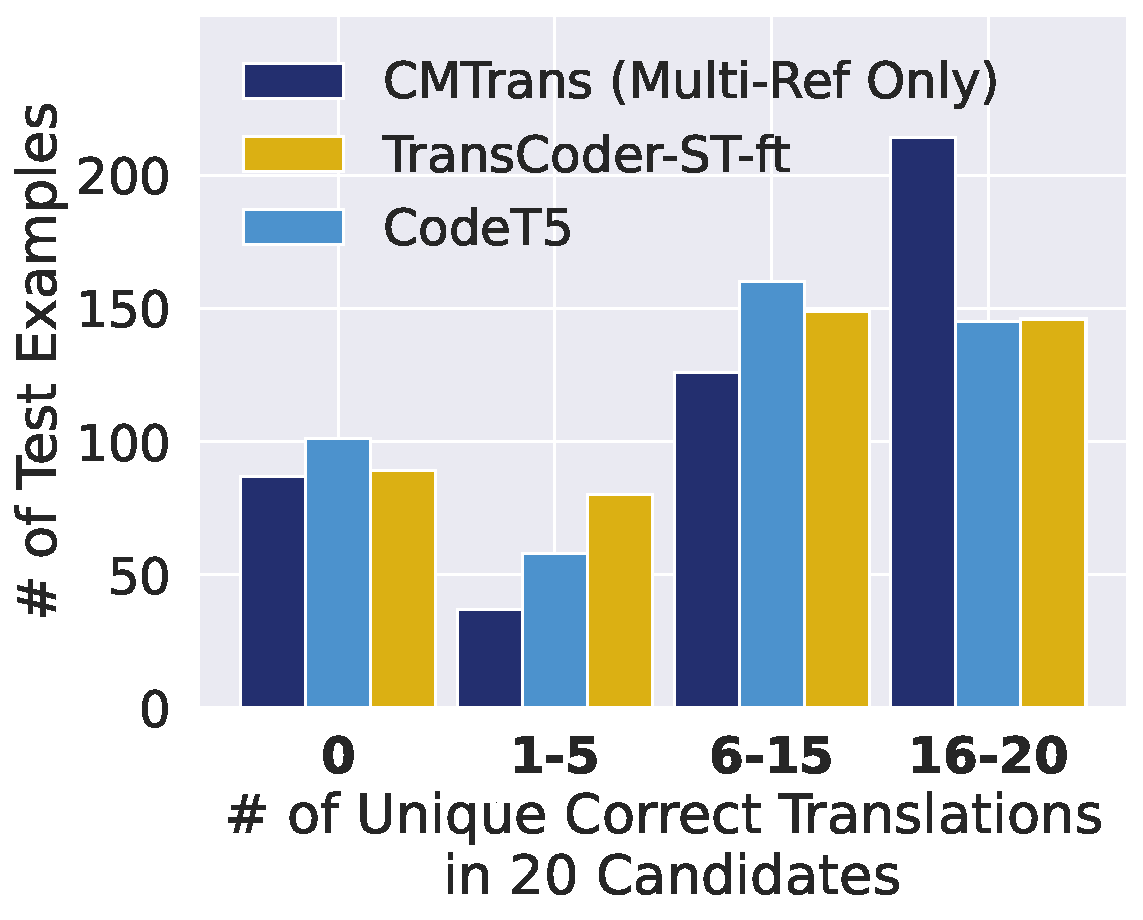
\includegraphics[width=\linewidth]{CMTrans_figs/unique_java2python.pdf}
  \caption{Java-to-Python}
  \label{fig:cmtrans_uni1}
\end{subfigure}\hfil % <-- added
\begin{subfigure}{0.4\linewidth}
  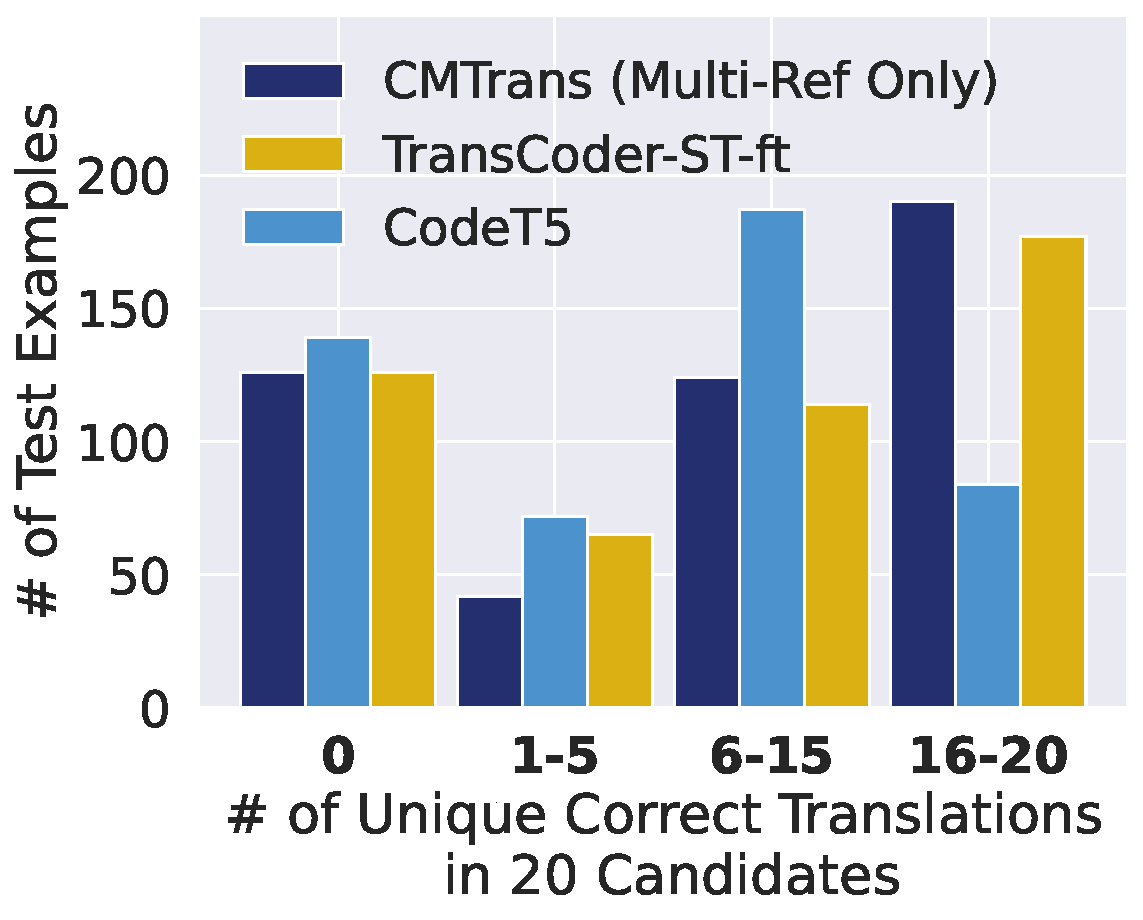
\includegraphics[width=\linewidth]{CMTrans_figs/unique_python2java.pdf}
  \caption{Python-to-Java}
  \label{fig:cmtrans_uni2}
\end{subfigure}
\caption{Number of unique correct translations in 20 candidates for each test example. We use beam search for each method, so the generated candidates are guaranteed to be distinct.}
\label{fig:cmtrans_unique}
\end{figure}




\begin{figure}
  \centering
  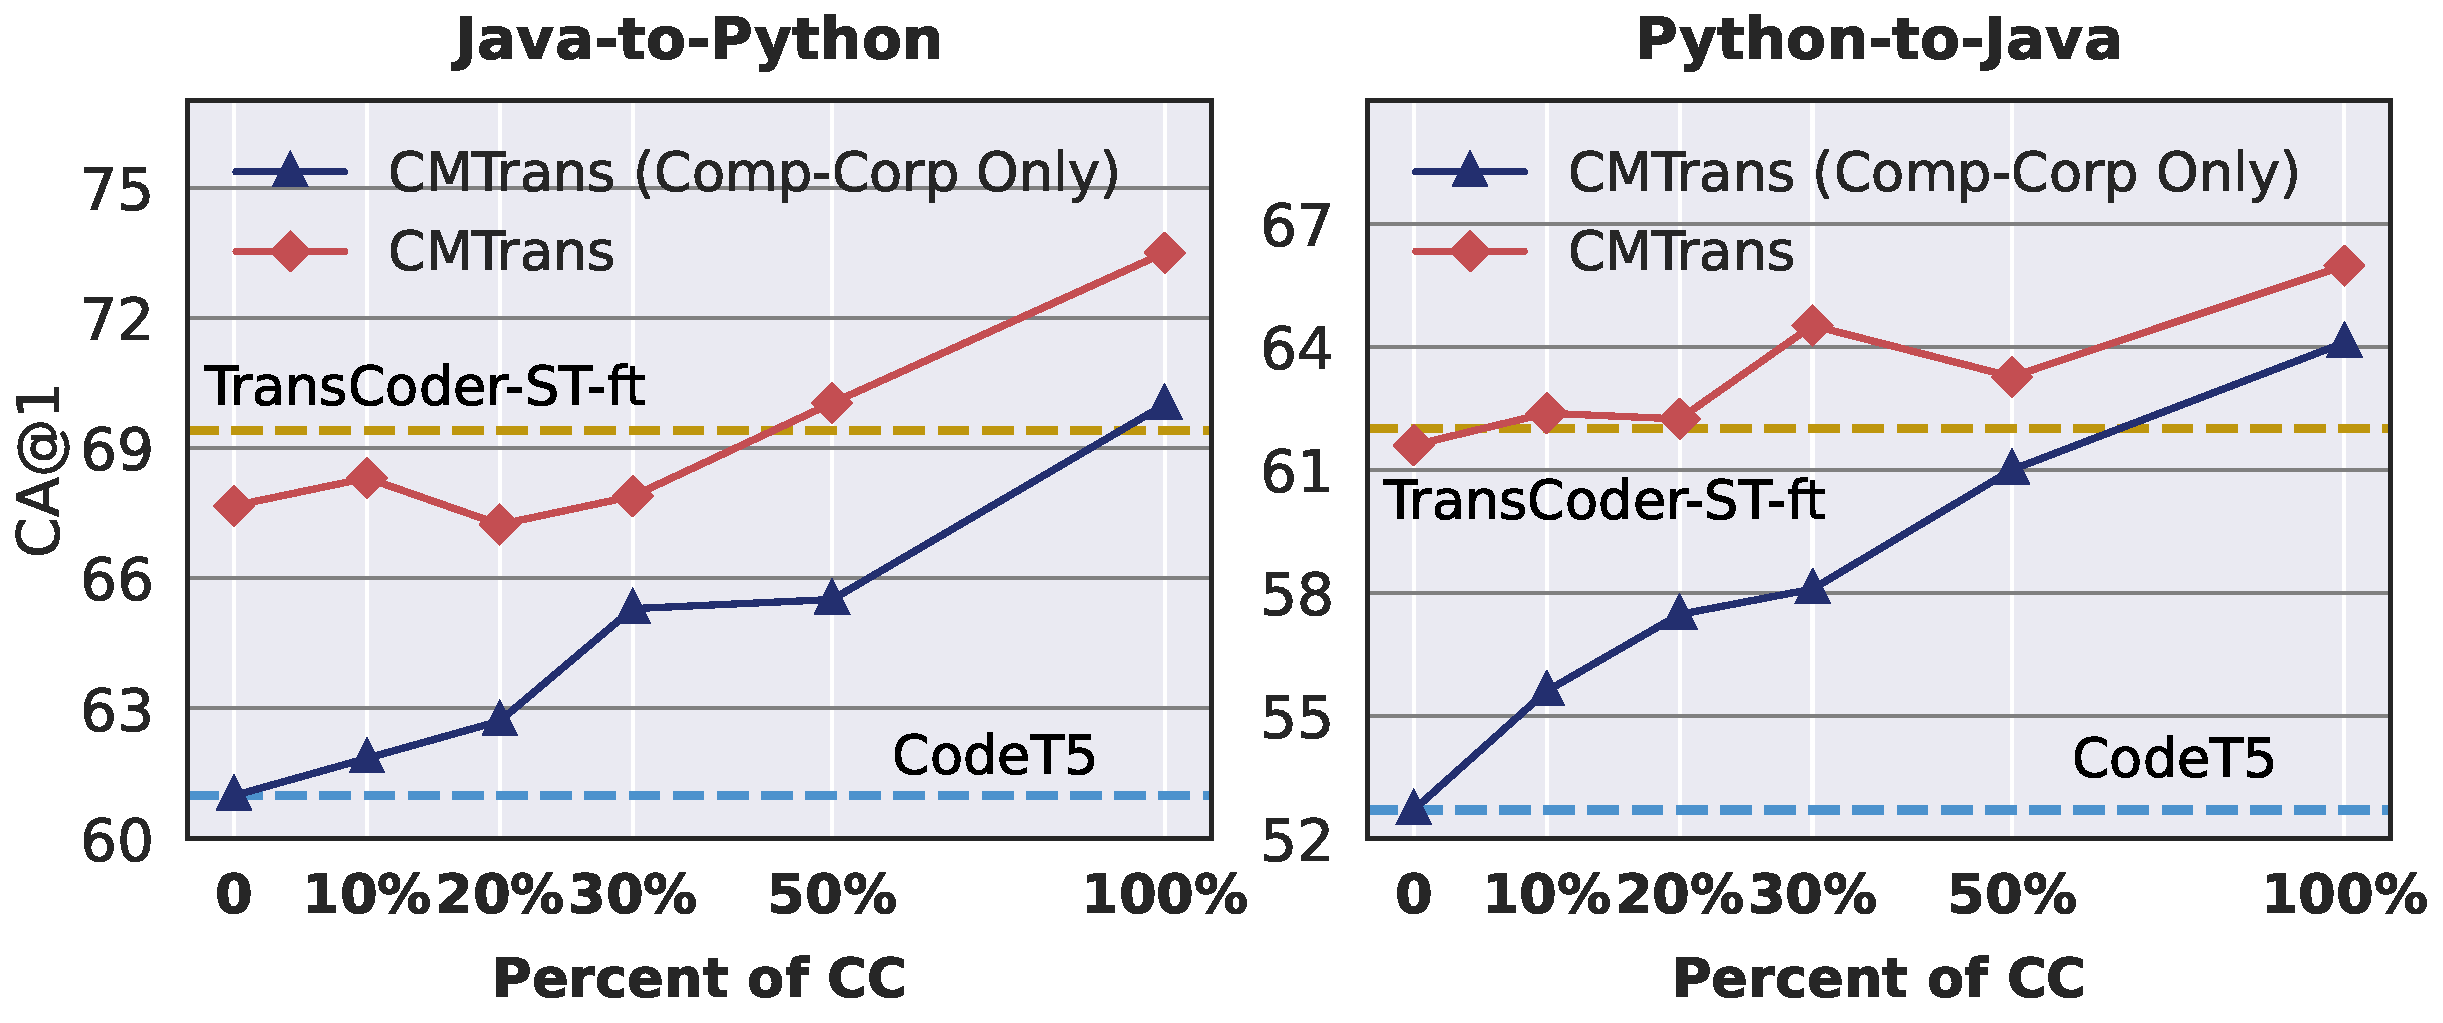
\includegraphics[width=0.7\linewidth]{CMTrans_figs/hyper_CC_analysis.pdf}
  \caption{Effect of the size of comparable corpora.}
  \label{fig:cmtrans_hyper_cc}
\end{figure}

\begin{figure}
  \centering
  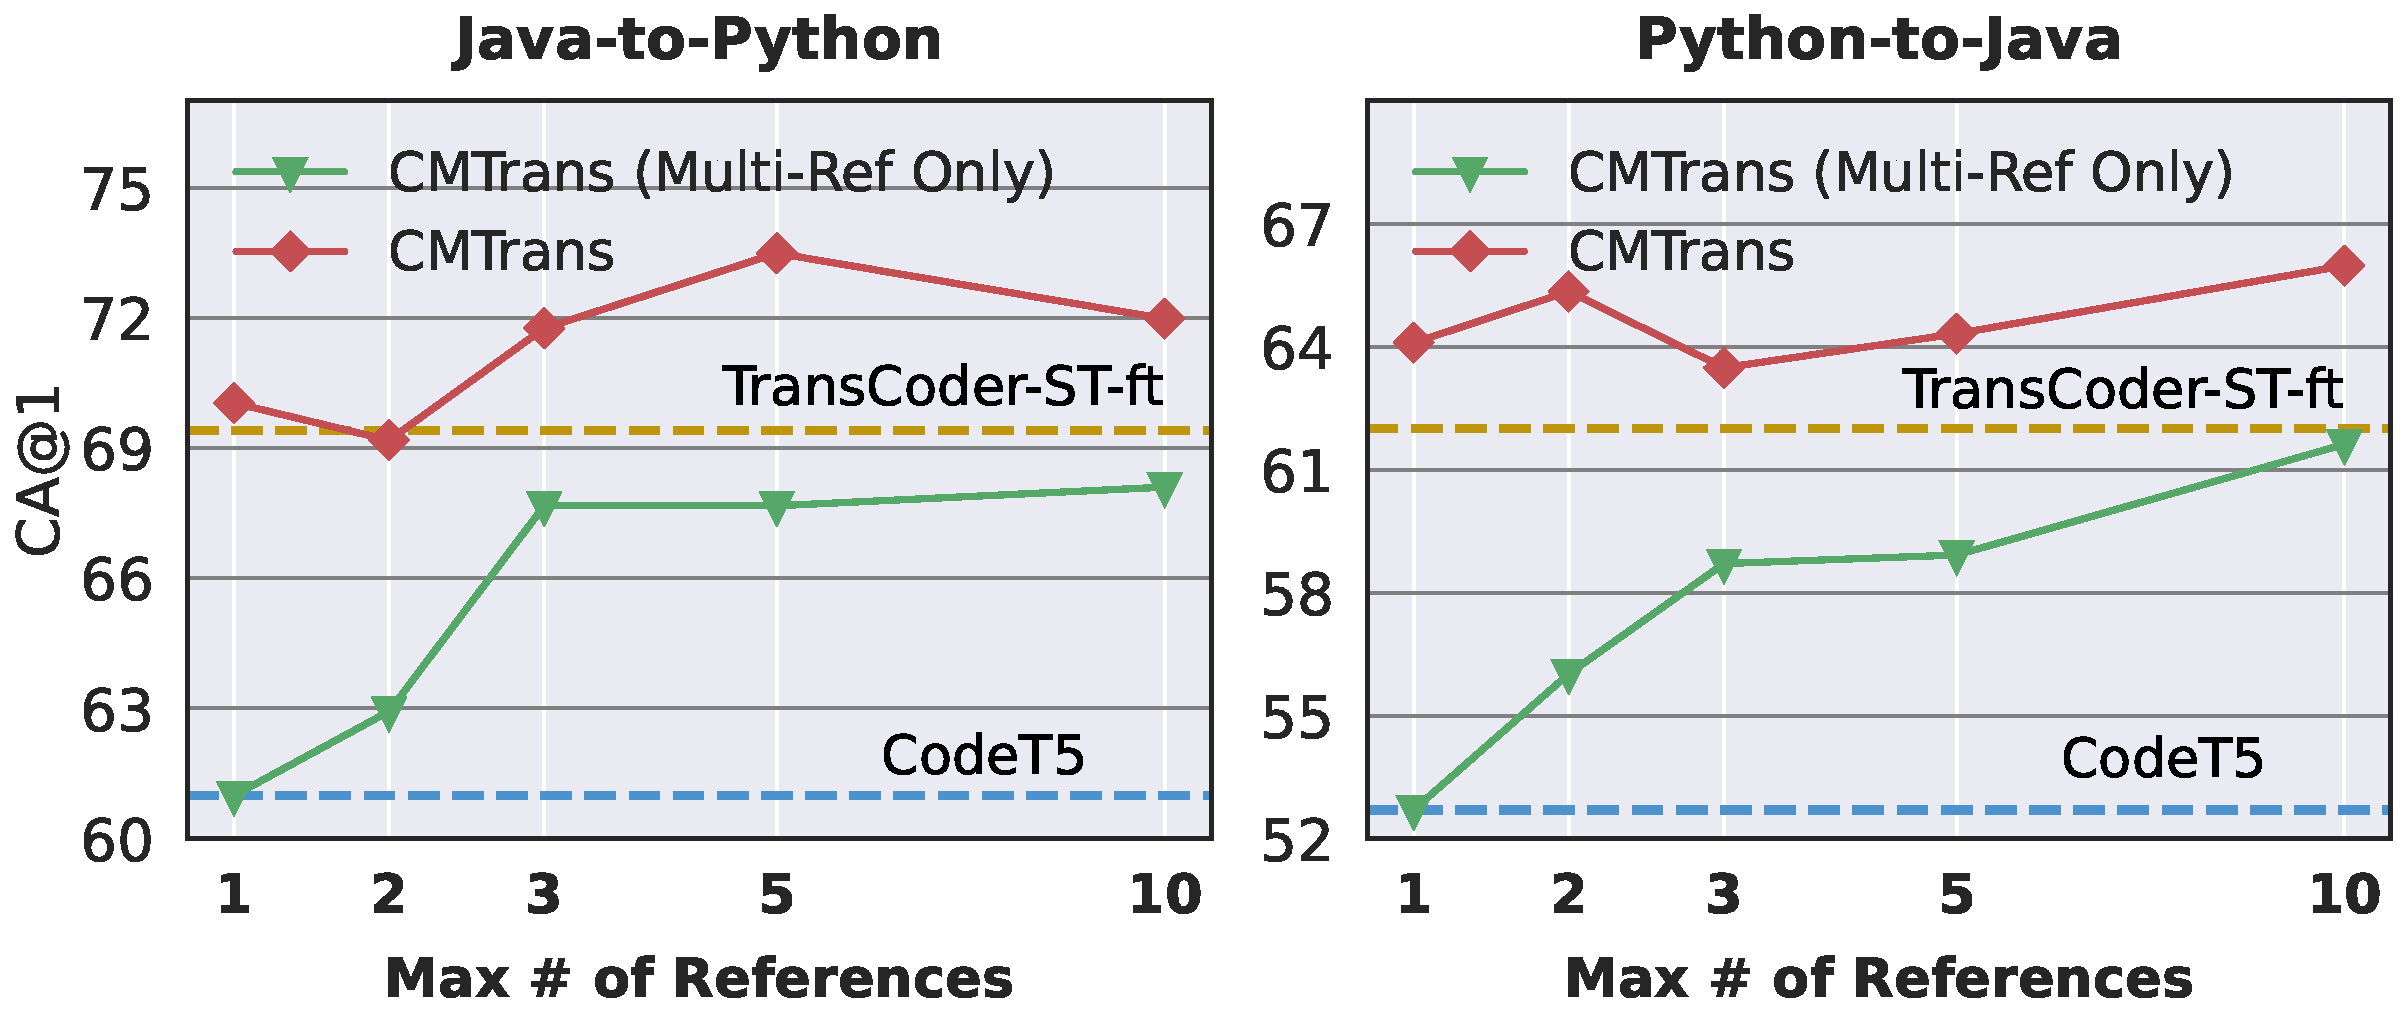
\includegraphics[width=0.7\linewidth]{CMTrans_figs/hyper_multi_analysis.pdf}
  \caption{Effect of the max number of references for each example.}
  \label{fig:cmtrans_hyper_multi}
\end{figure}

\subsection{Influence of Multiple References}
As for \textbf{RQ3}, we hypothesize that training on additional references can reduce overfitting to a single translation. 
To validate this hypothesis, we show in \autoref{fig:cmtrans_unique} that when trained with multiple references, \cmtransours can generate more unique correct translations using beam search within the same number of candidate outputs.
For instance, in Java-to-Python translation, there are 214 test examples where \cmtransours generates $\geq$ 16 unique translations, while there are only 145 and 146 examples for CodeT5 and TransCoder-ST-ft, respectively.
Furthermore, the scores under the ``0'' group indicate that after training with multiple references, the model generates at least one correct translation for more test examples.
In other words, in addition to CA@1, training CodeT5 on multiple references also improves on CA@20.

\subsection{Hyper-parameter analysis}
To answer \textbf{RQ4}, we analyze two hyper-parameters: 

\start{Size of comparable corpora}
We sample the same percentage of comparable examples from AVATAR-comp and Gen-comp and combine the sampled data.
\cmtransours is finetuned with at most 5 references in all trials.
As shown in \autoref{fig:cmtrans_hyper_cc}, as we increase the size of comparable corpora, \cmtransours (\CC Only) always has better performance.
While the trends are not monotonic for \cmtransours, it still obtains the best performance with full comparable corpora.

\start{Number of references}
We also examine the effect of the maximum number of references for each parallel example in finetuning.
We observe that the performance of \cmtransours does not always increase when finetuned with more references.
The reason might be that \cmtransours may generate more unique correct translations for some training examples than others.
As a result, the training signals the model received from different examples could be unbalanced, especially when the maximum number of references for each example is large.


\subsection{Case Studies}
We show a constructed comparable example in \autoref{fig:cmtrans_case}. 
% More case studies for comparable corpora and generated references can be found in Appendices~\ref{sec:app_case_cc} and \ref{sec:app_case_multi}.
As shown in \autoref{fig:cmtrans_case}, both the Java function extracted from GitHub and the generated Python function remove a config by name and return this config.
The only difference is the Java function obtains the name of each config by a helper function, while the generated Python function directly accesses the ``\texttt{name}'' attribute.
We also observe that this function is likely to belong to a large software project, which has a different nature from coding problems (e.g., the example in \autoref{fig:cmtrans_example_intro}).
As a result, combining collected and generated comparable examples provides diverse training signals to \cmtransours.

\begin{figure}[t]
    \centering
    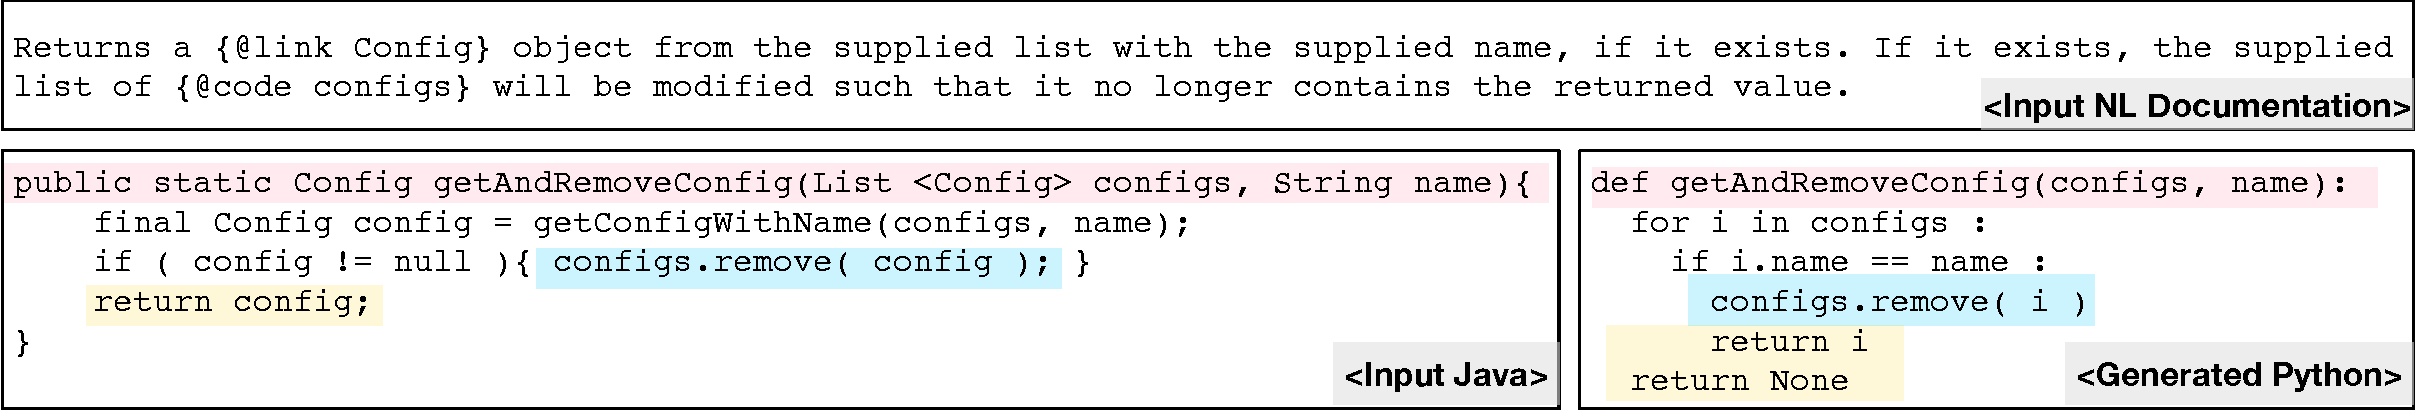
\includegraphics[width=\linewidth]{CMTrans_figs/case_short_fig_v2.pdf}
    \caption{Case study: a comparable example generated by our method with an NL-to-code generation model. We highlight the lines in the Java program and the generated Python program that can be matched.}
    \label{fig:cmtrans_case}
\end{figure}

\section{Chapter Summary}
In this chapter, we present two data augmentation techniques for code translation: comparable corpora and multiple references.
We study multiple ways of building comparable corpora, such as feeding natural language code documentation to code generation models.
Additionally, we generate multiple reference translations using \cmtransours and filter references using automatically generated unit tests.
Experiments on translation between 6 language pairs show that our two techniques improve CodeT5 substantially, by an average of 7.5\% CA@1.
The analyses further show that after training on comparable corpora, the model learns to generate more fluent code with the same types of constructs. With multiple references, the model learns to generate a larger number of unique correct translations.

While this chapter constructs scalable and effective training data for code translation, it focuses on \textbf{script-level} and \textbf{static} generation. Namely, the input and output are both code scripts, and the model generates code using one pass, without interacting with the environment.
The next chapter introduces the construction of scalable and effective training data for \textbf{repo-level} coding problems under the \textbf{coding agent} setting, which aims to generate code with real-world repositories as context. During inference, the model can interact with the environment by viewing files, editing files, executing bash commands, etc.. 






























\chapter{Constructing Scalable Coding Agent Training Environments with Sandbox Testing \textcolor{aquablue}{(\textit{completed})}}
\label{chap:repost}

\section{Introduction}
The previous chapter improves the scalability of script-level code translation data while remaining effective.
In this chapter, we construct scalable and effective repository-level (repo-level) coding agent training data by reducing the complexity of training environment construction.

% [motivate repo-level coding agent training]
Repo-level code generation aims to generate code with real-world, naturally occurring repositories as context, which aligns well with real-world software development.
However, most existing repo-level training datasets still treat code generation as a traditional sequence prediction task~\cite{codesearchnet,swebench}, neglecting the executable nature of code generation: the feedback can be obtained from execution.
In comparison, existing script-level code generation methods leverage execution feedback to improve model training~\cite{NEXT,plum,RLTF}.
They leverage online coding platforms as a natural resource to build large-scale algorithm problem datasets with test cases.
Such execution feedback is useful in constructing training targets~\citep{NEXT,plum} or reward signals~\citep{RLTF,exp_refine}.


While online coding platforms serve as a natural resource for large-scale algorithm problem datasets with test cases, it is non-trivial to build \textbf{execution-based} datasets for \textbf{repo-level} code generation at a \textbf{large scale}.
One major challenge is to set up executable environments.
Existing repo-level datasets typically conduct \textit{integration testing} that executes test files inside the repositories, which requires building the entire repository~\citep{swebench,R2E}.
As shown in prior research, this setup process is extremely challenging~\citep{super}, which may include installing external packages, determining execution context (e.g., relative import), debugging installation errors or runtime errors, etc.
Hence, existing methods for coding environment construction either require huge manual effort \citep{repocoder,swebench,swegym} or, when automated, suffer from low success rate~\citep{R2E}, limiting the scale of resulting datasets.

\begin{figure}
  \centering
  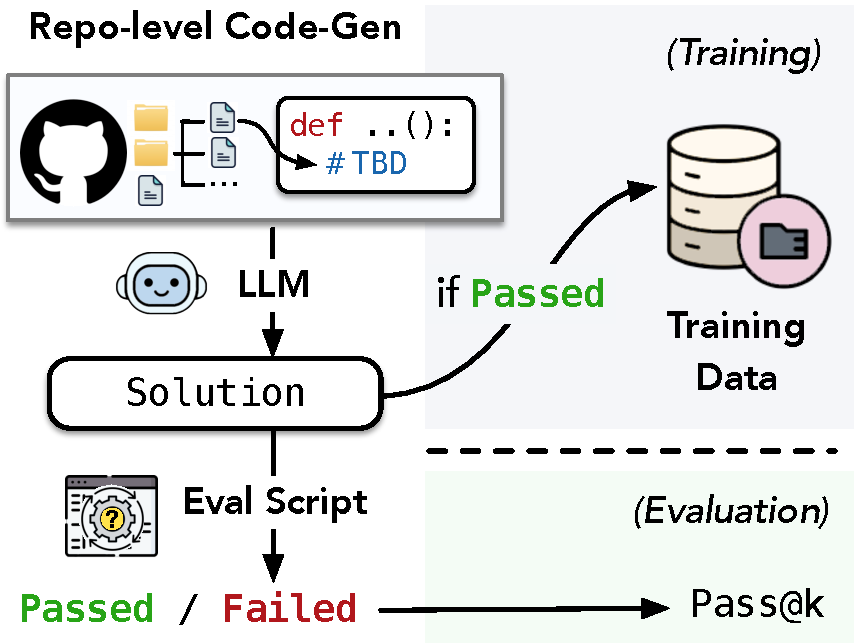
\includegraphics[width=0.6\textwidth]{RepoST_figs/intro.pdf}
  \caption{
    We can use the coding environments built by \repostmethodName for training and evaluation.
    We first apply the code generation model to generate candidate solutions with the original repository as context.
    Then we evaluate the solutions by executing the evaluation script built by \repostmethodName.
    For evaluation, we directly compute Pass@$k$ scores.
    For training, we add all successful solutions to the train set and further finetune the model.
  }
\label{fig:repost_intro}
\end{figure}

In this work, instead of integration testing, we present \repostmethodName, an \textbf{automated} framework to construct \textbf{Repo}-level coding environments with \textbf{S}andbox \textbf{T}esting.
Specifically, given a function in a GitHub repository, we sandbox the function and its local dependencies to a separate script and generate tests with an LLM.
To control the quality of the evaluation script, we iteratively resolve environment or runtime errors and improve test coverage.
We also conduct execution-based, AST-based, and LLM-based quality checks and only keep examples where the functionality of the sandboxed function does not alter and the tests are valid, reasonable, and have high coverage.
The resulting dataset allows us to obtain execution feedback in training and evaluation. 
As shown in \autoref{fig:repost_intro}, the models generate the target function with the entire GitHub repository as context. We then use the evaluation script to obtain execution feedback.

% [The method: RepoST]
Compared to integration testing used by previous datasets, we would like to highlight the benefits of sandbox testing in constructing \textbf{scalable} coding environments:
(1) In general, the external dependencies of a function are typically much simpler than those of a repository.
By isolating the function and its local dependencies, we can execute the function by \textit{only installing the necessary packages}.
(2) If any execution error occurs, we can debug the separate scripts \textit{without modifying the original repository}. This ensures that the datasets remain naturalistic: 
code generation models can still access the original, real-world repository.

% [Details of RepoST]
With the high scalability of our framework, we construct coding environment datasets for both training and evaluation: \reposttrainsetName and \repostevalsetName.
By the time the paper was published, \reposttrainsetName was the largest repo-level code generation dataset with execution support, with 7,415 functions sampled from 824 repositories.
The large scale enables training on \reposttrainsetName and evaluating on other benchmarks such as RepoEval~\citep{repocoder} or HumanEval~\citep{codex}.

% [Results on script-level code-gen]
Experiments show that by training on \reposttrainsetName, the method achieves performance gain on both algorithm problems in HumanEval~\citep{codex} and repo-level tasks in RepoEval~\citep{repocoder}.
For instance, we improve Qwen2.5-Coder by 5.5\% Pass@1 on HumanEval and 3.5\% Pass@1 on RepoEval and \repostevalsetName.

% [Results on SWE-Bench, SWT-Bench, and Commit-0, compared to the base model]
Note that \reposttrainsetName provides coding tasks based on real-world repositories that have execution feedback, it can also be applied to coding agent training~\citep{sweagent,openhands}.
For instance, after training on only 500 successful function generation trajectories sampled from \reposttrainsetName, we improve the resolved rates of Qwen2.5Coder-7B~\cite{qwen25coder} from 1.8\% to 7.8\% on the SWE-Bench issue-solving dataset~\cite{swebench}, from 0.23\% to 2.54\% on the SWT-Bench test generation dataset~\cite{swt-bench}, and from 4.80\% to 9.25\% on the Commit-0 library generation dataset~\cite{commit0}.


\section{Methodology}
The framework of \repostmethodName is illustrated in \autoref{fig:repost_framework}. 
After sampling GitHub repositories and extracting functions (\S\ref{sec:pre_curation}),
We sandbox each function and its local dependencies to a separate script (\S\ref{sec:sandboxing}), generate tests (\S\ref{sec:test_generation}), and conduct quality control on the executability of the scripts, the functionality of the sandboxed function, and the test quality (\S\ref{sec:quality_control}).
% We provide all the prompts in \S\ref{app:data-construction}.
When we use our environments to train (\S\ref{sec:code_gen_exps}) 
% and evaluate (\S\ref{sec:benchmarking_exps}) 
code generation models, the models can still access the original GitHub repository, and we provide execution feedback by executing the evaluation scripts.
To create user-friendly datasets, \textbf{we keep a shared Docker environment for all the evaluation scripts}.


\begin{figure}[t]
    \centering
    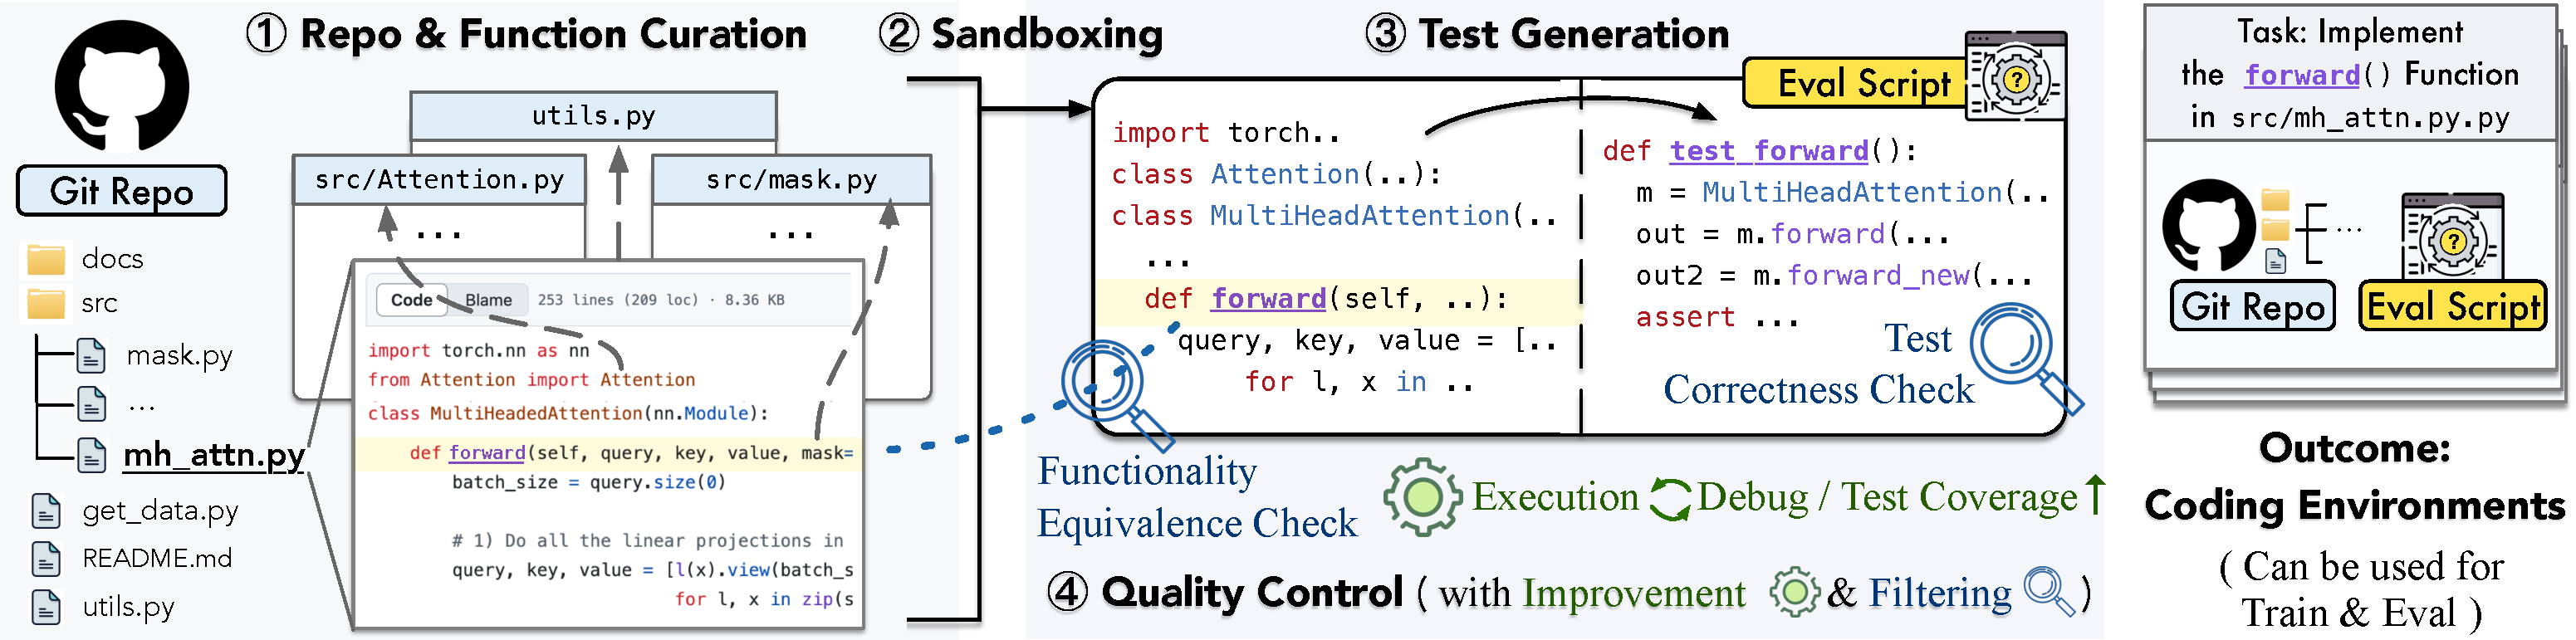
\includegraphics[width=\textwidth]{RepoST_figs/framework.pdf}
    \upv
    \caption{The \repostmethodName coding environment construction framework. We sandbox the target function and its dependencies to a separate evaluation script for execution, which avoids building the entire repository. We design careful quality control strategies with iterative quality improvement and post-filtering. The outcome of \repostmethodName is a set of executable repo-level coding environments, which can be used for training and evaluation.}
    \label{fig:repost_framework}
    \downv
\end{figure}


\subsection{Repository and Function Curation}
\label{sec:pre_curation}
We first randomly sample non-forked, MIT-licensed, Python GitHub Repositories with file sizes smaller than \texttt{10M}.
With the sandbox testing method, we are able to set up environments for individual functions and do not need to build the entire repository.
Hence, unlike previous works~\citep{R2E}, our method does not need to filter out repositories without setup files (e.g., \texttt{setup.py}).
The detailed repository statistics are provided in \S\ref{sec:dataset_stats}.


Then we extract functions from the repositories. 
To build the datasets in a docker with no access to GPUs or external services, we follow R2E~\citep{R2E} and filter out functions associated with GPUs, cloud tasks, etc. by keywords.
To balance the distribution of examples, we keep at most 30 functions for each repository.
After this step, for the train set, we started from 1,000 repositories and obtained 17,448 functions from 851 repositories.
For the evaluation set, we started from 200 repositories and obtained 1,043 functions from 139 repositories.
In theory, one can further scale up the dataset with more starting repositories.

\subsection{Sandboxing: Key to Environment Setup}
\label{sec:sandboxing}

\begin{figure}
  \centering
  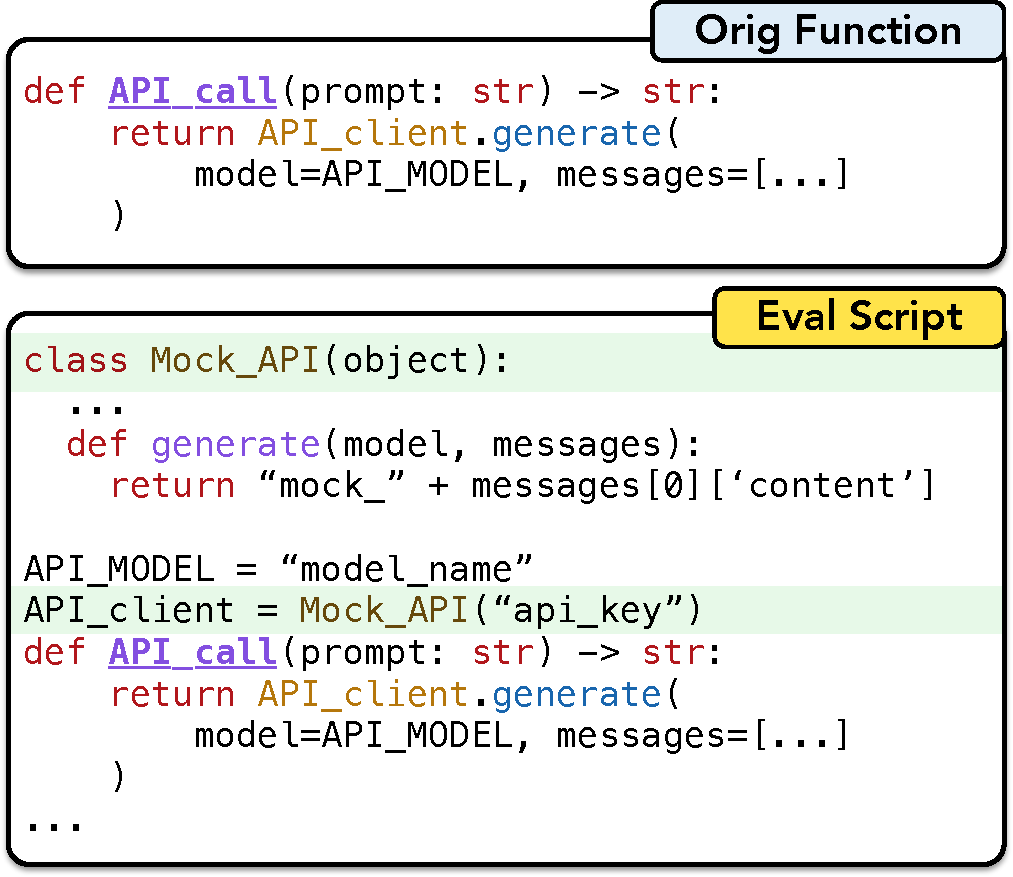
\includegraphics[width=0.6\linewidth]{RepoST_figs/sandboxing.pdf}
    \upv
  \caption{
    An example where the LLM successfully creates a mock class, \texttt{Mock\_API}, to replace real external API calls.
    In this way, while the function body of the target function \texttt{API\_call} remains exactly the same as in the original codebase,
    it can be executed without making real API calls.
  }
    \label{fig:repost_sandboxing}
    \downv
\end{figure}

It is non-trivial to create coding environments that provide correct execution feedback for the implementation of GitHub functions.
Existing methods typically provide execution feedback with integration testing, which creates test files that import the target function from the codebase. Executing such tests requires building the entire repository, which generally requires a complicated environment and is challenging for both human and LLMs.




With the observation that the external dependencies of a function are typically much simpler than a repository,
We tackle this challenge with \textbf{sandbox testing}, where we create a separate script containing the target function with the \textbf{exact same functionality} as the original one and the context that supports its executability.
By isolating the function and its local dependencies, we can execute the function by only installing the necessary packages.


\start{Sandboxing based on Local Dependencies}
The major challenge of sandboxing is to ensure the executability of the function.
While a standalone function can be directly copied to a separate script and executed, a typical GitHub function may depend on other modules, classes, or global variables in the same repository.
Thus, we leverage the call graph to extract such local dependencies that the target function directly or indirectly calls.
Then we combine all the code fragments into the context and prompt an LLM (e.g., GPT-4o) to aggregate all the code fragments into a single script, with as little editing as possible.


\start{Sandboxing External APIs and Files}
Even if all the dependencies are presented, it is still nontrivial to execute the sandboxed script if it requires external API, databases, files, etc. 
We explicitly prompt the LLM to create mock connections for any external API and create strings or write example files to a specific directory for file reading.
\autoref{fig:repost_sandboxing} presents a successful case of sandboxing with mock APIs.
% We provide examples of the generated sandboxed scripts in \Cref{fig:repost_case1-input,fig:repost_case1-sandbox,fig:repost_case1-tests,fig:repost_case2-input,fig:repost_case2-sandbox,fig:repost_case2-tests}.
% % \S\ref{app:case-studies}.


\start{Functionality Equivalence Control}
In addition to executability, another challenge of sandboxing is to ensure that the target function's functionality does not alter.
We first conduct a list of sanity checks on the function name, length of scripts, etc., and re-generate examples that do not satisfy the requirements.
We also have a final quality control step (in \S\ref{sec:quality_control}) that compares the functionality of the sandboxed and original functions.
The precision of quality control is further verified in the human study in \S\ref{sec:human_study}.


\subsection{Test Generation}
\label{sec:test_generation}

\start{Equivalence Testing}
We generate synthetic tests in the sandboxed script to evaluate the correctness of the generated code.
Specifically, we prompt the LLM to (1) generate a set of test inputs to the target function and (2) conduct equivalence testing that checks whether the function generated in evaluation has the same behavior as the sandboxed function (i.e., the ``ground-truth'' implementation).
Compared to traditional methods that specify the I/O examples in the test cases~\citep{codex}, equivalence testing does not need to predict the expected outputs and is more feasible for LLMs~\citep{R2E}.


\start{Test Generation with Mock APIs and Files}
We observe that the LLM is able to generate tests with the mock classes created in the sandboxing step as context. 
% As shown in \Cref{fig:repost_case2-input,fig:repost_case2-sandbox,fig:repost_case2-tests}, 
As shown in \autoref{fig:repost_sandboxing}, we create mock class instances as the test inputs and still ensure that the function body of the sandboxed function remains the same as the original function.

\start{Test Quality Control}
Similarly to the sandboxing step, for quality control purposes, we conduct a series of sanity checks, such as requiring the test function to call the target function and have at least 3 assertions.
% (see \autoref{tab:sanity_check_test_gen} for the full list). 
We further check the coverage and correctness of the tests in the final quality control step (\S\ref{sec:quality_control}), 


\subsection{Quality Control and Filtering}
\label{sec:quality_control}

We conduct quality control for the executability of the evaluation script, the functionality of the sandboxed function, and the test quality.

\start{Iterative Execution and Debugging}
In principle, if the model-generated function is exactly the same as the ground truth, the evaluation scripts should be successfully executed, with all the tests passed.
Hence, we execute the examples sequentially in a docker. If there are any execution errors or if the ground truth implementation cannot pass any test cases, we provide the error message as the context and prompt an LLM to debug the evaluation script. Examples that still have errors after $k$ execution-debugging iterations are filtered out.

We also dynamically install external packages during execution.
During execution, if there are any \texttt{ModuleNotFound} errors, we extract the package names from the error message, run a \texttt{pip install} command, and execute the script again.
In case the package name differs from the import name or the code requires a specific version of packages, we also allow the LLM to output package installation commands during debugging.
In this way, we are able to install external packages for functions extracted from repositories without setup files.


\start{Iterative Test Coverage Improvement}
To ensure that the test functions cover the major functionality of the target functions, we further compute the branch coverage rate of all the evaluation scripts.
If the branch coverage rate is lower than some threshold (we set $80\%$ for the train set and $100\%$ for the evaluation set),
We provide the LLM with the missing lines and prompt it to improve the test function by incorporating more tests.


\start{Final-Step Quality Check \& Filtering}
As a final step, we conduct two quality checks: functionality equivalence check and test correctness check, and filter out unqualified examples. 


To ensure the validity of sandbox testing, we examine the \textbf{functionality equivalence} between the sandboxed and original function.
We first compare the AST of the function bodies, which is a sufficient condition of functionality equivalence. 
In our resulting dataset, 81.7\% of the examples have the same AST. The remaining ones are filtered out from the evaluation set. 
To include more examples in the train set, 
since it is also possible that code with the same functionality has different ASTs (e.g., HTML tags can be parsed with \texttt{LexborHTMLParser} and \texttt{BeautifulSoup}),
We prompt an LLM~\footnote{The original code could be inexecutable due to package installation errors (e.g., \texttt{BeautifulSoup} in this case), so we do not execute the original code.} to compare the functionality equivalence, which is shown to have high agreement with human (see our human study in \S\ref{sec:human_study} for details).
We also include the examples that pass the LLM check for the train set.


In principle, a test that calls the target function without any assertion checks still has a 100\% coverage rate.
We hence conduct \textbf{test correctness} check and apply an LLM to check whether the tests are correct, reasonable, and complete the verification of the functionality. Human study in \S\ref{sec:human_study} demonstrates the high precision of the LLM test correctness checker.


\begin{table}[t]
\centering
\resizebox{0.7\linewidth}{!}{
\begin{tabular}{lrrcc}
\toprule
\textbf{Dataset} & \textbf{\#Ex} & \textbf{\#Repo} & \textbf{Repo?} & \textbf{AutoTest?} \\
\midrule
HumanEval & 164 & -- & \xmark & \xmark \\
DS1000 & 1,000 & -- & \xmark & \xmark \\
ClassEval & 100 & -- & \xmark & \xmark \\
RepoEval-Func & 455 & 6 & \cmark & \xmark \\
SWE-Bench & 2,294 & 12 & \cmark & \xmark \\
CoderEval & 230 & 43 & \cmark & \xmark \\
DevEval & 1,874 & 117 & \cmark & \xmark \\
EvoCodeBench & 275 & 25 & \cmark & \xmark \\
SWE-Gym & 2,438 & 11 & \cmark & \xmark \\
R2E-Eval1 & 246 & 137 & \cmark & \cmark \\
R2E (Reproduced) & 744 & 123 & \cmark & \cmark \\
\midrule
\textbf{\reposttrainsetName} & \textbf{7,415} & \textbf{824} & \cmark & \cmark \\
\textbf{\repostevalsetName} & 296 & 99 & \cmark & \cmark \\
\bottomrule
\end{tabular}
}
\caption{Statistics of \reposttrainsetName and \repostevalsetName compared to existing \textbf{execution-based} code generation datasets. 
R2E (Reproduced) applies the R2E method to the same set of input repositories as \reposttrainsetName, but results in a smaller number of repositories and examples.
``Repo?'' and ``Auto Test?'' refer to the repo-level setting and automatically generated tests.}
\label{tab:repost_stats}
\end{table}

\begin{table}[t]
\centering
\resizebox{0.7\textwidth}{!}{
\begin{tabular}{lcc}
\toprule
\bf Avg Stats.
& \textbf{\textsc{Train}} 
& \textbf{\textsc{Eval}} \\
\midrule
Target \# Tokens (Lines) & 112.4 (12.8) & 102.7 (9.9) \\
Eval Script \# Tokens (Lines) & 842.5 (75.7) & 1217.5 (122.3) \\
\# Test Cases & 5.7 & 8.2 \\
Test Branch Coverage & 97.8\% & 100\% \\
\% Standalone Functions & 28.1\% & 26.4\% \\
\# External Libraries & 894 & 106 \\
\bottomrule
\end{tabular}
}
\caption{Detailed statistics of our datasets.}
\label{tab:repost_detailed_stats}
\end{table} 


\begin{table}[t]
\centering
\resizebox{0.4\linewidth}{!}{
\begin{tabular}{l|cc|cc}
\toprule
\textbf{Check} & \multicolumn{2}{c|}{\textbf{Func}} & \multicolumn{2}{c}{\textbf{Test}} \\
\cmidrule(lr){2-3} \cmidrule(lr){4-5}
Human $\rightarrow$ & Yes & No & Yes & No \\
\midrule
GPT-4o: Yes & 13 & 0 & 9 & 1 \\
GPT-4o: No & 1 & 6 & 4 & 6 \\
\bottomrule
\end{tabular}
}
\caption{Agreement between human and GPT-4o on checking (1) the functionality equivalence between the sandboxed and original function, and (2) the test correctness.
When GPT-4o predicts ``Yes'' for both quality checks, it has a high agreement with human.}
\label{tab:repost_agreement}

\end{table}

\begin{table}[t]
\centering
\resizebox{0.5\linewidth}{!}{
\begin{tabular}{ccc}
\toprule
\textbf{\% Solved} & \textbf{\% Use-Tool} & \textbf{Easy / Med / Hard} \\
\midrule
81.5\% & 59.3\% & 29.6 / 51.9 / 18.5 \\
\bottomrule
\end{tabular}
}
\caption{Human study results. We ask the participants to complete the function with the same context we use to evaluate code generation models in \S\ref{sec:code_gen_exps}.}
\label{tab:repost_human_study_1}
\end{table}




\section{Resulting Datasets: \reposttrainsetName and \repostevalsetName}
\label{sec:dataset_stats}

\start{Statistics}
We build a train set, \reposttrainsetName, and an evaluation set, \repostevalsetName.
To reduce contamination, we build \reposttrainsetName from repositories created between \texttt{2023-01-31} and \texttt{2024-08-31},
and build \repostevalsetName from repositories created after \texttt{2024-09-01}.


We compare the statistics of the datasets and existing \textit{execution-based} datasets in \autoref{tab:repost_stats}.
By the time the paper was published, \reposttrainsetName was the largest repo-level dataset with execution feedback.
Prior works such as RepoEval~\citep{repocoder} or SWE-Gym~\citep{swegym} require huge human effort to set up the environments.
Automated frameworks such as R2E~\citep{R2E} apply LLMs to the complicated task of building the entire repositories and suffer from low success rates.
In comparison, \repostmethodName only requires necessary dependencies for each function, which is more feasible for LLMs and benefits scalability.




\autoref{tab:repost_detailed_stats} shows detailed statistics of our datasets.
Our datasets achieve high test numbers and branch coverage rates with iterative test coverage improvement and quality filtering.
Results also show that \repostmethodName can create relatively complex examples in terms of length and local and external dependencies.
The percentage of standalone functions (i.e., functions without local dependencies) are 28.1\% and 26.4\% in our datasets. Both are very close to 27\%, the percentage of standalone functions among all GitHub code estimated by \citet{deveval}.





\subsection{Quality Verification with Human Study}
\label{sec:human_study}

\start{Agreement between LLM Checker and Human}
We conduct a human study to verify the precision of our LLM-based quality check strategies introduced in \S\ref{sec:quality_control}.
We ask 3 computer science graduate students to conduct functionality equivalence and test correctness checks for
20 examples sampled from \repostevalsetName (before the final filtering), with the same instruction we use to prompt the LLM checkers.
The Kappa agreement scores among human annotators are 0.9179 for the functionality check and 0.7750 for the test check.

Results in \autoref{tab:repost_human_study_1} show that all 13/20 examples that pass GPT-4o's functionality check are also predicted as ``same functionality'' by human.
Among 10 examples that pass GPT-4o's test quality check, 9 of them are predicted as ``high-quality tests'' by human.
It demonstrates that after applying our filtering strategies for quality control, the remaining examples have high quality.
In principle, one can further enhance dataset quality by manually inspecting and selecting the examples.
% We provide more details about the experiments in \S\ref{app:human-study-details}.





\start{Solvability Check}
We conduct another human study to check whether the examples are reasonable and can be solved by human.
We assigned 27 examples constructed by \repostmethodName to 9 computer science students, with no overlaps, and asked them to complete the function and answer questions about the difficulties of the examples.
% (see \S\ref{app:human-study-details} for details).

Results show that 81.5\% of the examples were solved by human, indicating that most examples are reasonable and not too complicated.
The remaining examples were not solved for various reasons, such as the participant is not familiar with the task (e.g., reading html data) or related libraries (e.g., \texttt{BeautifulSoup4}), the intent of the function cannot be fully entailed from the context, etc.
% Towards the unclear intent issue, we designed an experiment in \S\ref{sec:benchmarking_exps}, where we generated additional instructions to improve the clarity.
We also observe that the generated examples have varying complexity levels based on the usage of external tools and the difficulty ratings.
Furthermore, 33.3\% of the examples
are solved in the first submission and 37.0\% require more than 5 submissions to solve. 




\section{Code Generation Training Experiments}
\label{sec:code_gen_exps}
\start{Training with \reposttrainsetName} 
In standard supervised fine-tuning (\textbf{SFT}), we can train the model with the code context $c$ as the input and the ground truth target function $f^*$ as the output.
The execution feedback provided by our \repostmethodName evaluation scripts further allows us to employ the \textbf{rejection sampling fine-tuning (RFT)} algorithm to generate additional valid training targets.
Specifically, we apply the model itself to our dataset, generating $n$ candidate solutions for each function based on its code context: $(c, f_1), \ldots (c, f_n)$. The method is denoted as \textbf{RFT (Self)}.
We can also apply other stronger models to generate candidates (denoted as \textbf{RFT (Distill)}). 
Only solutions that pass our test cases are retained.
We then finetune the model on the successful functions $(c, f_1'), \ldots (c, f_m')$ and the ground truth $(c, f^*)$ using the standard negative log-likelihood loss.

To obtain more training pairs for both the ``Self'' and ``Distill'' settings, we further prompt the model itself or a stronger model to debug the failed solutions, with the error message in the context.
We also train the model on successfully debugged solutions $(c, f_1''), \ldots (c, f_k'')$.





\begin{table}[t]
\centering
\resizebox{0.8\textwidth}{!}{
\begin{tabular}{lcccccc}
\toprule
\multirow{2}{*}{\textbf{Model}}  
& \multicolumn{2}{c}{\bf HumanEval} 
& \multicolumn{2}{c}{\textbf{RepoEval-Func}} 
& \multicolumn{2}{c}{\bf \repostevalsetName} \\
\cmidrule(lr){2-3}
\cmidrule(lr){4-5}
\cmidrule(lr){6-7}
& Pass@$1$ & $\Delta$ & Pass@$1$ & $\Delta$ & Pass@$1$ & $\Delta$ \\
\midrule
StarCoder2-7B~\citep{starcoder2} 
& 34.76 & -- & 32.98 & -- & 26.35 & -- \\
\quad + SFT 
& 37.20 & \small{\colordg{$\uparrow$2.44}} 
& 33.78 & \small{\colordg{$\uparrow$0.80}}
& 27.70 & \small{\colordg{$\uparrow$1.35}} \\
\quad + RFT (Self) 
& 39.63 & \small{\colordg{$\uparrow$4.87}}
& 34.58 & \small{\colordg{$\uparrow$1.61}}
& 28.38 & \small{\colordg{$\uparrow$2.03}} \\
\quad + RFT (Distill) 
& \textbf{40.24} & \bf \small{\colordg{$\uparrow$5.49}}
& \textbf{35.12} & \bf \small{\colordg{$\uparrow$2.14}}
& \textbf{29.05} & \bf \small{\colordg{$\uparrow$2.70}} \\
\midrule
Qwen2.5-Coder-7B~\citep{qwen25coder} 
& 79.27 & -- & 38.06 & -- & 29.39 & -- \\
\quad + SFT 
& 80.48 & \small{\colordg{$\uparrow$1.21}} 
& 39.94 & \small{\colordg{$\uparrow$1.88}} 
& 30.74 & \small{\colordg{$\uparrow$1.35}} \\
\quad + RFT (Self) 
& \bf 84.76 & \bf \small{\colordg{$\uparrow$5.49}} 
& 40.75 & \small{\colordg{$\uparrow$2.69}} 
& 31.76 & \small{\colordg{$\uparrow$2.36}} \\
\quad + RFT (Distill) 
& \bf 84.76 & \bf \small{\colordg{$\uparrow$5.49}} 
& \bf 41.55 & \bf \small{\colordg{$\uparrow$3.49}} 
& \bf 32.43 & \bf \small{\colordg{$\uparrow$3.04}} \\
\bottomrule
\end{tabular}
}
\caption{Code generation training results. We evaluate Pass@1 for all experiments. For RepoEval, we use the ``Oracle'' repo-level context as used in their original paper.
}
\label{tab:repost_main}
\end{table}


\subsection{Experimental Setup} 
\start{Datasets and Evaluation Metrics}
We train two models: StarCoder2-7B~\citep{starcoder2} and Qwen2.5-Coder-7B~\citep{qwen25coder} with \reposttrainsetName and evaluate on two public benchmarks: HumanEval~\citep{codex}, an algorithm problem dataset, and RepoEval~\citep{repocoder}, a repo-level code generation dataset. We also evaluate on \repostevalsetName.
For RepoEval, we only evaluate on the ``function'' split, which supports execution. We use the ``Oracle'' context to mitigate the bias of context retrieval methods.
We report the Pass@1 scores on all datasets.
% More evaluation details are provided in \S\ref{app:training-exp-details}.


\start{Training Details}
We compare three training methods: SFT, RFT (Self), and RFT (Distill).
For the ``Distill'' method, we apply GPT-4o and Claude-3.5-Sonnet to generate and debug candidate solutions, separately, and combine their successful candidates for training.
% We provide the number of examples where we obtained at least one successful solution in \autoref{tab:rej_sampling_stats}.
% Other details are shown in \autoref{app:training-exp-details}.


\subsection{Experimental Results}
\start{Main Results}
\autoref{tab:repost_main} demonstrates that models trained with \reposttrainsetName can generalize well to other public benchmarks.
Specifically, we improve Qwen2.5-Coder by 5.5\% Pass@1 on HumanEval, 3.5\% on RepoEval-Func, and 3.0\% on \repostevalsetName.
Furthermore, in all experiments, training with RFT, even with self-training only, achieves better performance than finetuning on the original GitHub function only.
For instance, RFT (Distill) outperforms SFT by 4.3\% Pass@1 on HumanEval.
This shows the benefit of training with environments that can provide execution feedback.
We can also observe that RFT with self-training in general has lower performance than distilling from stronger models. 
% As shown in \autoref{tab:rej_sampling_stats}, 
Particularly,
We can only obtain 1573 additional training targets with StarCoder2, but we obtained 3606 by combining GPT-4o and Claude-3.5.
We hypothesize that one can obtain more examples and hence achieve better performance by sampling with more candidate solutions, generating from different types of context, etc., and we leave that to future work.




\start{Scaling Law Analysis}
In \autoref{fig:repost_scaling_law}, we investigate how the scale of training data affects model performance. 
Specifically, we randomly sample different numbers of examples from \reposttrainsetName to train the model.
We can see that the performance of RFT (Distill) increases as we scale up the training data, which suggests the advantage of training data with high scalability.
Furthermore, with different scales of data, RFT consistently achieves better performance than SFT, which further demonstrates the effectiveness of training environments with execution feedback.



\begin{figure}
  \centering
  \begin{subfigure}[b]{0.4\textwidth}
    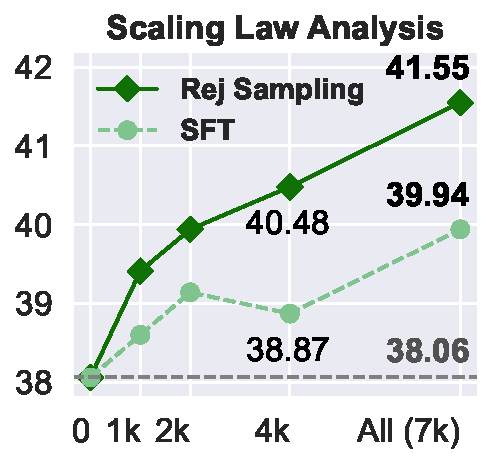
\includegraphics[width=\textwidth]{RepoST_figs/scaling_law.pdf}
    \caption{Scaling law analysis.}
    \label{fig:repost_scaling_law}
  \end{subfigure}
  \hspace{0.4cm}
  \begin{subfigure}[b]{0.32\textwidth}
    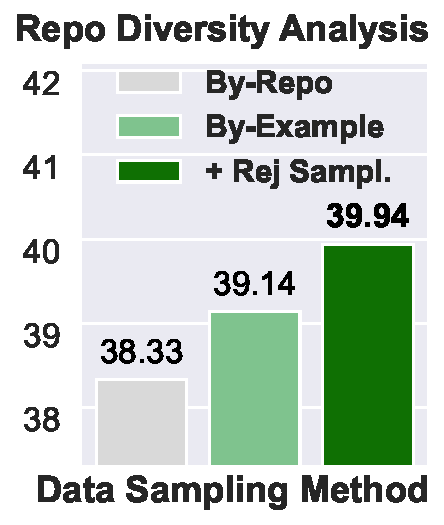
\includegraphics[width=\textwidth]{RepoST_figs/repo_diversity.pdf}
    \caption{Repo diversity.}
    \label{fig:repost_diversity_study}
  \end{subfigure}
  \caption{(a) Pass@1 scores on RepoEval with different numbers of training examples.
  (b) Pass@1 scores on RepoEval with different methods to sample 2,000 training examples. 
  Sample-by-Example has a broader repository coverage and achieves better Pass@1. The performance is further enhanced with RFT (Distill).
  }
  \label{fig:repost_analysis}
\end{figure}


\start{Repository Diversity Experiment}
\autoref{fig:repost_diversity_study} examines whether broader repository coverage leads to better performance, given a fixed budget of training examples.
We fix the number of examples to 2,000 and experiment with two example sampling methods: (1) Sample-by-Repo, where we keep sampling repositories and adding all the functions in the repository to the training set, until the data size reaches 2,000; (2) Sample-by-Example, which is the same setting as \autoref{fig:repost_scaling_law}, where we randomly sample functions from \reposttrainsetName.
We observe that Sample-by-Example, covering 678 repositories, outperforms Sample-by-Repo, which only covers 221. The performance is further improved by RFT.
Recall that our method only needs to set up individual functions, compared to existing methods, such as R2E, that need to build the entire repository, it is much easier to build datasets with broad repository coverage with our method, which benefits model training.




\section{Coding Agent Training Experiments}
In this section, we show that in addition to static code generation models, \reposttrainsetName can also be used to train coding agents.

\subsection{Experimental Setup}
\start{Training Coding Agents with \reposttrainsetName}
We formulate the training task as follows: given a GitHub repository and the path to a function in it, whose body has been masked out, the agent needs to implement this function based on a piece of textual description.

To set up the task, we run a Docker container for each \reposttrainsetName instance. We clone the GitHub repository and checkout to the specific commit. The target function would be masked properly before applying the agent to solve the task.
Then we apply the agent to complete the masked function.
After it finishes, we extract the function body it generates (if any), and run \repostmethodName's evaluation script to verify its correctness.

Finally, similar to \autoref{sec:code_gen_exps}, we train the agent model with rejection sampling finetuning: we apply the teacher model on a set of training instances, evaluate the results, and train the model on the collection of successful trajectories with supervised finetuning.

\start{Training Details}
In this experiment, we use Claude-3.7~\cite{claude37} as the teacher model and train Qwen2.5-Coder-7B as the student model. We use OpenHands~\cite{openhands} (v0.40.0) as the agent scaffold.
To limit the cost of generating training trajectories, we only generate 500 successful trajectories with Claude-3.7 for training.

\start{Evaluation Datasets and Metrics}
We report the resolved rates on three repo-level coding agent benchmarks: the SWE-Bench Verified issue-solving benchmark~\cite{swebench}, the SWT-Bench Verified test generation benchmark~\cite{swt-bench}, and the Commit-0 library construction benchmark~\cite{commit0}.
Note that none of the benchmarks specifically targets function generation. Namely, the experiment is under the zero-shot task generalization setting.

\subsection{Experimental Results}
\autoref{tab:repost-agent} presents the results of training the Qwen2.5-Coder-7B agent on 500 trajectories generated from \reposttrainsetName.
Results show that although \reposttrainsetName does not target issue-solving, test generation, or library construction, the finetuned agent significantly outperforms the base model in all three benchmarks.
Particularly, we improve the performance of Qwen2.5Coder-7B from 1.8\% to 7.8\% on SWE-Bench Verified, from 0.23\% to 2.54\% on SWT-Bench Verified, and from 4.80\% to 9.25\% on Commit-0 Lite.
This demonstrates that the \repostmethodName training environments are also effective in training coding agents.
Note that we only train the agent on 500 successful trajectories (generated from around 1200 \reposttrainsetName instances) due to computational budget.
It is possible to generate a larger training set based on the entire \reposttrainsetName dataset. We leave the exploration to future work.


\begin{table}[t]
\centering
\small
\resizebox{0.8\columnwidth}{!}{%
\begin{tabular}{l ccc}
\toprule
\bf Methods & \bf SWE-Bench & \bf SWT-Bench & \bf Commit-0 \\
 & Resolved \% & Resolved \% & Resolved \% \\
\midrule
Qwen2.5Coder-7B & 1.8 & 0.23 & 4.80 \\
+ \reposttrainsetName (500) RFT 
& \bf 7.8~{\textcolor{treegreen}{$\uparrow$6.0}} 
& \bf 2.54~{\textcolor{treegreen}{$\uparrow$2.31}} 
& \bf 9.25~{\textcolor{treegreen}{$\uparrow$4.45}} \\
\bottomrule
\end{tabular}%
}
\caption{Performance of the Qwen2.5Coder-7B agent on SWE-Bench Verified, SWT-Bench Verified, and Commit-0 Lite before and after training. 
}
\label{tab:repost-agent}
\end{table}








% \section{Related Work}

% \start{Code Generation Training}
% Existing works have shown the effectiveness of pretraining~\citep{codellama,starcoder2,deepseekcoder} or instruction tuning~\citep{wei2023magicoder,wizardcoder,dsR1} on real-world code.
% To further finetune models for code generation, existing works have built large-scale training datasets with test cases by leveraging large-scale online algorithm problems.
% The execution feedback from test cases is used in constructing training targets~\citep{NEXT,plum} or reward signals~\citep{RLTF,exp_refine}.
% As repo-level code generation, existing works such as SWE-Gym~\citep{swegym} build training environments by manually setting up dependencies and configurations for the entire GitHub repositories.
% The repository setup process is complicated and challenging to automate, resulting in limited dataset scales.
% In comparison, we design a sandbox testing method that only requires setting up the necessary dependencies for individual GitHub functions, which reduces the difficulty of environment setup and leads to better scalability.

% \start{Code Generation Benchmarks}
% Execution-based benchmarks have been widely adopted for code generation, which provide test cases to evaluate the generated code~\citep{codex,APPS,MBPP}.
% Researchers have built benchmarks with large test coverage~\citep{evalplus}, multiple languages~\citep{multiple}, diverse domains~\citep{DS1000,classeval}, etc. LiveCodeBench~\citep{livecodebench} periodically extracts newly released algorithm problems, which enables contamination-free evaluation.

% To assess the models' ability on repo-level coding tasks, recent works leverage repositories with test cases to build benchmarks on code patch generation~\citep{repocoder,codebenchgen}, issue solving~\citep{swebench}, test generation~\citep{testgeneval}, test execution~\citep{execution-agent}, environment setup~\citep{super}, etc.
% Recent works aim to provide live evaluation manually~\citep{evocodebench} or leverage an LLM to set up the repository environment and generate test cases.
% However, both methods require building the entire repository, which is challenging for both human and LLMs and limit the scale of the resulting datasets.
% \repostmethodName improves the scalability with sandbox testing and enables the construction of live benchmarks from naturally occurring repositories.






\section{Chapter Summary}
In this chapter, we present \repostmethodName, a scalable method to construct environments for code generation in real-world repositories that support sandbox testing.
\repostmethodName is fully automatic and enables the construction of scalable execution-based training environments and live benchmarks.
Experiments demonstrate that training with the resulting train set, \reposttrainsetName, leads to performance gain on other public benchmarks. For instance, we improve Qwen2.5Coder by 5.49\%/3.49\% Pass@1 on HumanEval/RepoEval.

While both \autoref{chap:cmtrans} and \autoref{chap:repost} focus on training and evaluation for one single task, we would like to note that the application of coding agents can be diverse in real-world usage. We will explore the generalizability to a wide range of coding agent tasks in \autoref{part:generalizability}.

% While both \autoref{chap:cmtrans} and \autoref{chap:repost} focus on reducing the difficulty of obtaining training data and thereby improving scalability, they do not study the other factor of training outcome: the effectiveness of each training instance. We will explore this direction in \autoref{chap:effective-analysis}.









\part{Training Coding Agents that Generalize across Tasks}
\label{part:generalizability}


\start{Overview of Part~\ref{part:generalizability}}
\autoref{part:scalability} presented two works for constructing scalable training data while preserving effectiveness. 
However, both works only focus on training and evaluation for a single task, whereas real-world coding agents are applied to a diverse set of applications.


In this part, we construct scalable training data for \emph{general-purpose coding agents} that generalize across a broad range of downstream tasks
This part contains two chapters.
In both chapters, we first conduct an in-depth analysis of the capabilities that the agent has not yet learned, but are required across diverse downstream tasks. 
Then we derive training data design principles based on the analysis results.

In \autoref{chap:hybrid-gym}, we investigate the transferable skills shared across diverse tasks by decomposing trajectories into fine-grained components (e.g., repository exploration) and derive a set of principles for training task design, such as matching the output format of downstream tasks and requiring non-trivial repository exploration.
Guided by these principles, we build our dataset on a set of scalable synthetic tasks, for instance, function localization and dependency search.
Experiments show that agents trained on our synthetic tasks effectively generalize to diverse real-world tasks (e.g., issue-solving, test generation, and library construction) that are not presented in the training data.

While \autoref{chap:hybrid-gym} presents principles for training task design, we observe that the concrete approach to accomplish the task is also crucial for training.
Particularly, experiments show that even successful trajectories generated from the same set of instances may have substantially different impacts in training.
In a \proposedWork (\autoref{chap:effective-analysis}), we propose a new work that aims to present principles for training trajectories.
We first conduct an analysis to investigate the characteristics that make a training trajectory beneficial or harmful in training from two aspects: the high-level problem-solving strategies and the concrete actions taken by the agent.
Then, we propose two trajectory augmentation methods to inject beneficial characteristics into the trajectories and remove harmful ones.













\chapter{Training General-Purpose Coding Agents with Scalable Tasks \textcolor{aquablue}{(\textit{completed})}}
\label{chap:hybrid-gym}



\begin{figure*}[t]
\centering
\resizebox{\linewidth}{!}{%
  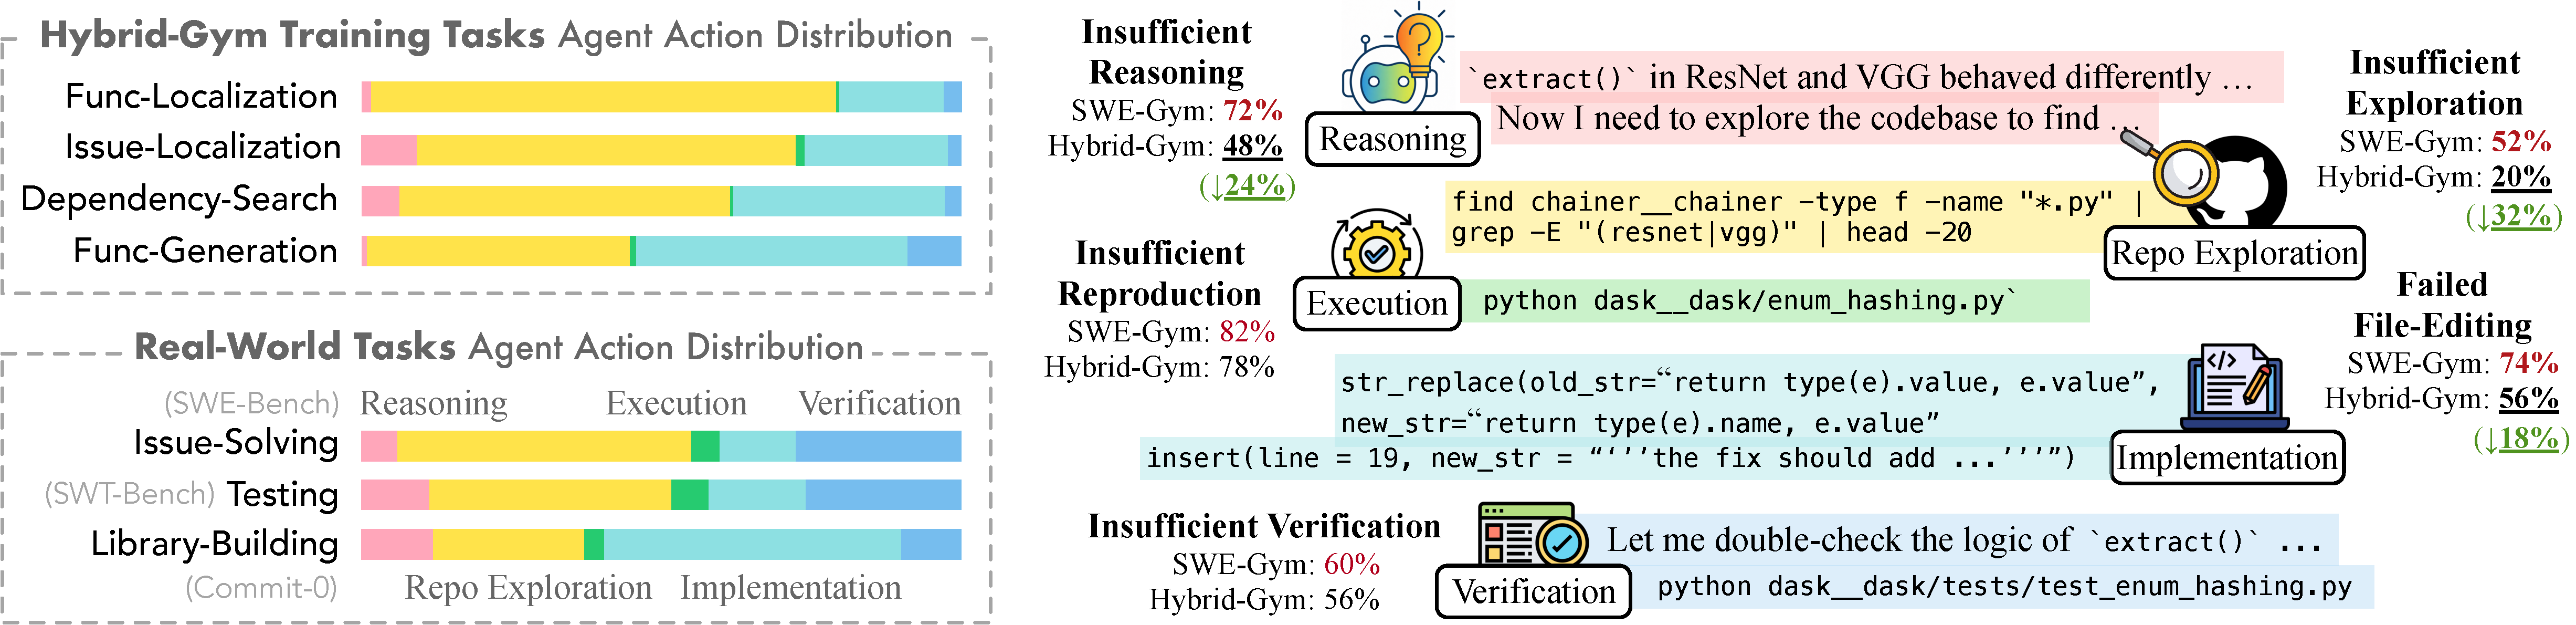
\includegraphics{HybridGym_figs/intro.pdf}%
}
\caption{(\textit{\textbf{Left}}) We decompose general coding agent tasks into a set of intermediate components and compute the percentage of agent actions spent on each component. Our training tasks partially cover verification and fully cover reasoning, repository exploration, and implementation, which consist of around 68\% of the actions.
\textit{(\textbf{Right})} Example actions for each component. Compared to a baseline training method, SWE-Gym~\cite{swegym}, training with our \repostmethodname significantly reduces failures due to insufficient reasoning, insufficient exploration, and failed file editing, improving the final resolved rate on SWE-Bench Verified from 10.6\% to 15.0\%. 
}
\label{fig:intro}
\end{figure*}

\section{Introduction}

% [Para-1: an overview of coding agent and its training]
Recent advances in large language models have enabled LM-based agents~\citep{sweagent,openhands} to tackle real-world coding tasks, with rapid progress in benchmarks such as the SWE-Bench issue resolution benchmark~\citep{swebench}.
While most existing methods only focus on the issue-solving task~\citep{swegym,R2EGym,swe-smith}, the application of coding agents can be diverse in real-world usage. A recent study show that more than 70\% of the real-world prompts target other software engineering tasks~\citep{valerie-interaction}.

% [Para-2: motivate task transfer]
As shown in a concurrent work~\citep{swe-play}, training on a single task can lead to overfitting and is not sufficient for generalizing to general coding agent tasks.
In particular, agents trained on issue solving do not transfer reliably to tasks such as test generation or library implementation. This calls for training coding agents with stronger \textbf{task generalization} capabilities.
Yet, in the current literature, task transferability for coding agents remains underexplored. 
In this work, we ask: what commonalities do real-world coding tasks share? How can we design training tasks that transfer effectively across a broad range of coding agent tasks?

% [Para-4: our analysis results]
To answer these questions, we start by decomposing real-world tasks into intermediate components (e.g., reasoning and repo-exploration) and analyzing the model's capabilities on each.
These results are shown in \autoref{fig:intro}.
We observe that a large number of actions in successful trajectories are spent on reasoning, repo-exploration, and implementation.
These categories also remain challenging for current coding agents.
For instance, even after finetuning on issue-solving~\cite{swegym}, the agent still has file editing failures for the majority of the examples.

Fortunately, these intermediate components can be isolated from the construction of coding environments with executable repositories (e.g., with all Python packages required by the repository installed).
In previous work, setting up executable repositories is often viewed as a prerequisite for constructing training examples. This typically involves a series of complex steps such as package installation and test generation, which is still challenging for agents~\cite{swe-play} and time-consuming for human~\cite{swegym,swe-smith,R2EGym}.
Based on the observation from our analysis, we ask: \textbf{can we design a set of tasks that cover the major components for coding practice: reasoning, repo-exploration, and implementation, but do not require executable repository setup?}


% [parap-5: in this paper]
In this paper, we present \repostmethodname, a large-scale coding agent training dataset containing a suite of coding agent training tasks that only require simple environment setup.
Based on our analysis summarized in \autoref{fig:intro}, we present a list of principles for training task design: the task needs to 
(1) match the output format of downstream tasks;
(2) include a repository exploration process; and 
(3) require non-trivial reasoning.
For scalability concerns, we further require that the task (4) must \emph{not} require a complicated environment setup.
Example tasks include function localization, issue localization, dependency search, and function generation.
As shown in \autoref{fig:intro}, even without setting up executable repositories, all our tasks cover the major intermediate components of multiple downstream tasks, and such components are achieved with a similar set of actions across tasks. 
After training on \repostmethodname, the agent has significantly lower failure rates in reasoning, exploration, and file-editing compared to the baseline training method~\cite{swegym}.


% [para-6: experimental results]
We conduct experiments on three real-world coding agent tasks: SWE-Bench issue-solving~\citep{swebench}, SWT-Bench test generation~\citep{swt-bench}, and Commit-0 library generation~\citep{commit0}.
Without training on any of the downstream tasks, \repostmethodname demonstrates strong task transferability on all three tasks, improving Qwen2.5Coder-32B by 25.4\% / 7.9\% / 5.1\% on SWE-Bench Verified / SWT-Bench Verified / Commit-0 Lite, which achieves comparable performance to in-domain datasets (i.e., data built for the downstream tasks). 
Additionally, we also improve the performance of training on existing in-domain datasets by combining with \repostmethodname (e.g., we improve SWE-Play~\citep{swe-play} by 2.4\% / 4.9\% on SWE-Bench Verified / SWT-Bench Verified).


% [para-7: controlled experiment results]
To provide insights to future research on coding agent training, we conduct a series of controlled experiments to reveal what transfers and what does not for coding agents.
In addition to validating our task design principles that require output format matching, repo-exploration, and non-trivial reasoning, we observe that even successful trajectories of the same set of instances can lead to markedly different impact.
Repository diversity improves training effectiveness, but training on the same repositories used in evaluation does not inflate performance gains.
The results emphasize the importance of teacher model selection and data selection.





\begin{table}[t]
\centering
\resizebox{\linewidth}{!}{%
\begin{tabular}{llcccc@{\hspace{4pt}\vrule width 0.6pt\hspace{4pt}}ccc}
\toprule
\bf Command & \bf Example & \bf Func-Localize & \bf Issue-Localize & \bf Dep-Search & \bf Func-Gen & \bf SWE-Bench & \bf SWT-Bench & \bf Commit-0 \\
\midrule
grep & \texttt{grep -i "pipeline"} & 31.3\% & 36.1\% & 48.4\% & 89.9\% & 35.4\% & 37.4\% & 5.3\% \\
find & \texttt{find . -type f -name "least\_angle.py"}           & 17.5\% & 11.1\% & 21.4\% & 8.7\%  & 16.2\% & 21.5\% & 31.6\% \\
cd   & \texttt{cd /workspace/scikit-learn}                       & 21.9\% & 31.5\% & 2.0\%  & 0.0\%  & 26.7\% & 0.0\% & 5.3\% \\
ls   & \texttt{ls -la}                                           & 6.6\%  & 2.3\%  & 3.7\%  & 0.0\%  & 2.4\%  & 12.4\% & 36.8\% \\

\bottomrule
\end{tabular}%
}
\caption{The use of Linux commands for repository exploration in our proposed training tasks (left) and downstream tasks (right). We show the percentage of each command used in the agent steps targeting repository exploration.
}
\label{tab:cmd-category}
\end{table}


\begin{table}[t]
\centering
\resizebox{\textwidth}{!}{%
\begin{tabular}{lcccc@{\hspace{4pt}\vrule width 0.6pt\hspace{4pt}}ccc}
\toprule
\bf Category & \bf Func-Localize & \bf Issue-Localize & \bf Dep-Search & \bf Func-Gen & \bf SWE-Bench & \bf SWT-Bench & \bf Commit-0 \\
\midrule
Analysis and reasoning        & 1.6\%  & 9.3\%  & 6.3\%  & 0.9\%  & 6.0\%  & 11.4\% & 1.3\% \\
Repository exploration        & 77.9\% & 66.2\% & 55.5\% & 44.6\% & 49.1\% & 40.3\% & 27.3\% \\
Execution of existing code    & 0.1\%  & 0.3\%  & 0.1\%  & 0.2\%  & 4.7\%  & 6.3\%  & 3.7\% \\
Solution implementation       & 17.4\% & 23.9\% & 35.3\% & 45.3\% & 12.7\% & 16.2\% & 53.8\% \\
Solution verification         & 3.0\%  & 0.3\%  & 2.8\%  & 9.0\%  & 27.6\% & 25.9\% & 10.9\% \\
\bottomrule
\end{tabular}%

}
\caption{We categorize the agent's actions based on the intermediate components of the task, where the categories are pre-defined. 
}
\label{tab:action-category}
\end{table}

\begin{figure}[t]
\centering
\resizebox{\linewidth}{!}{%
  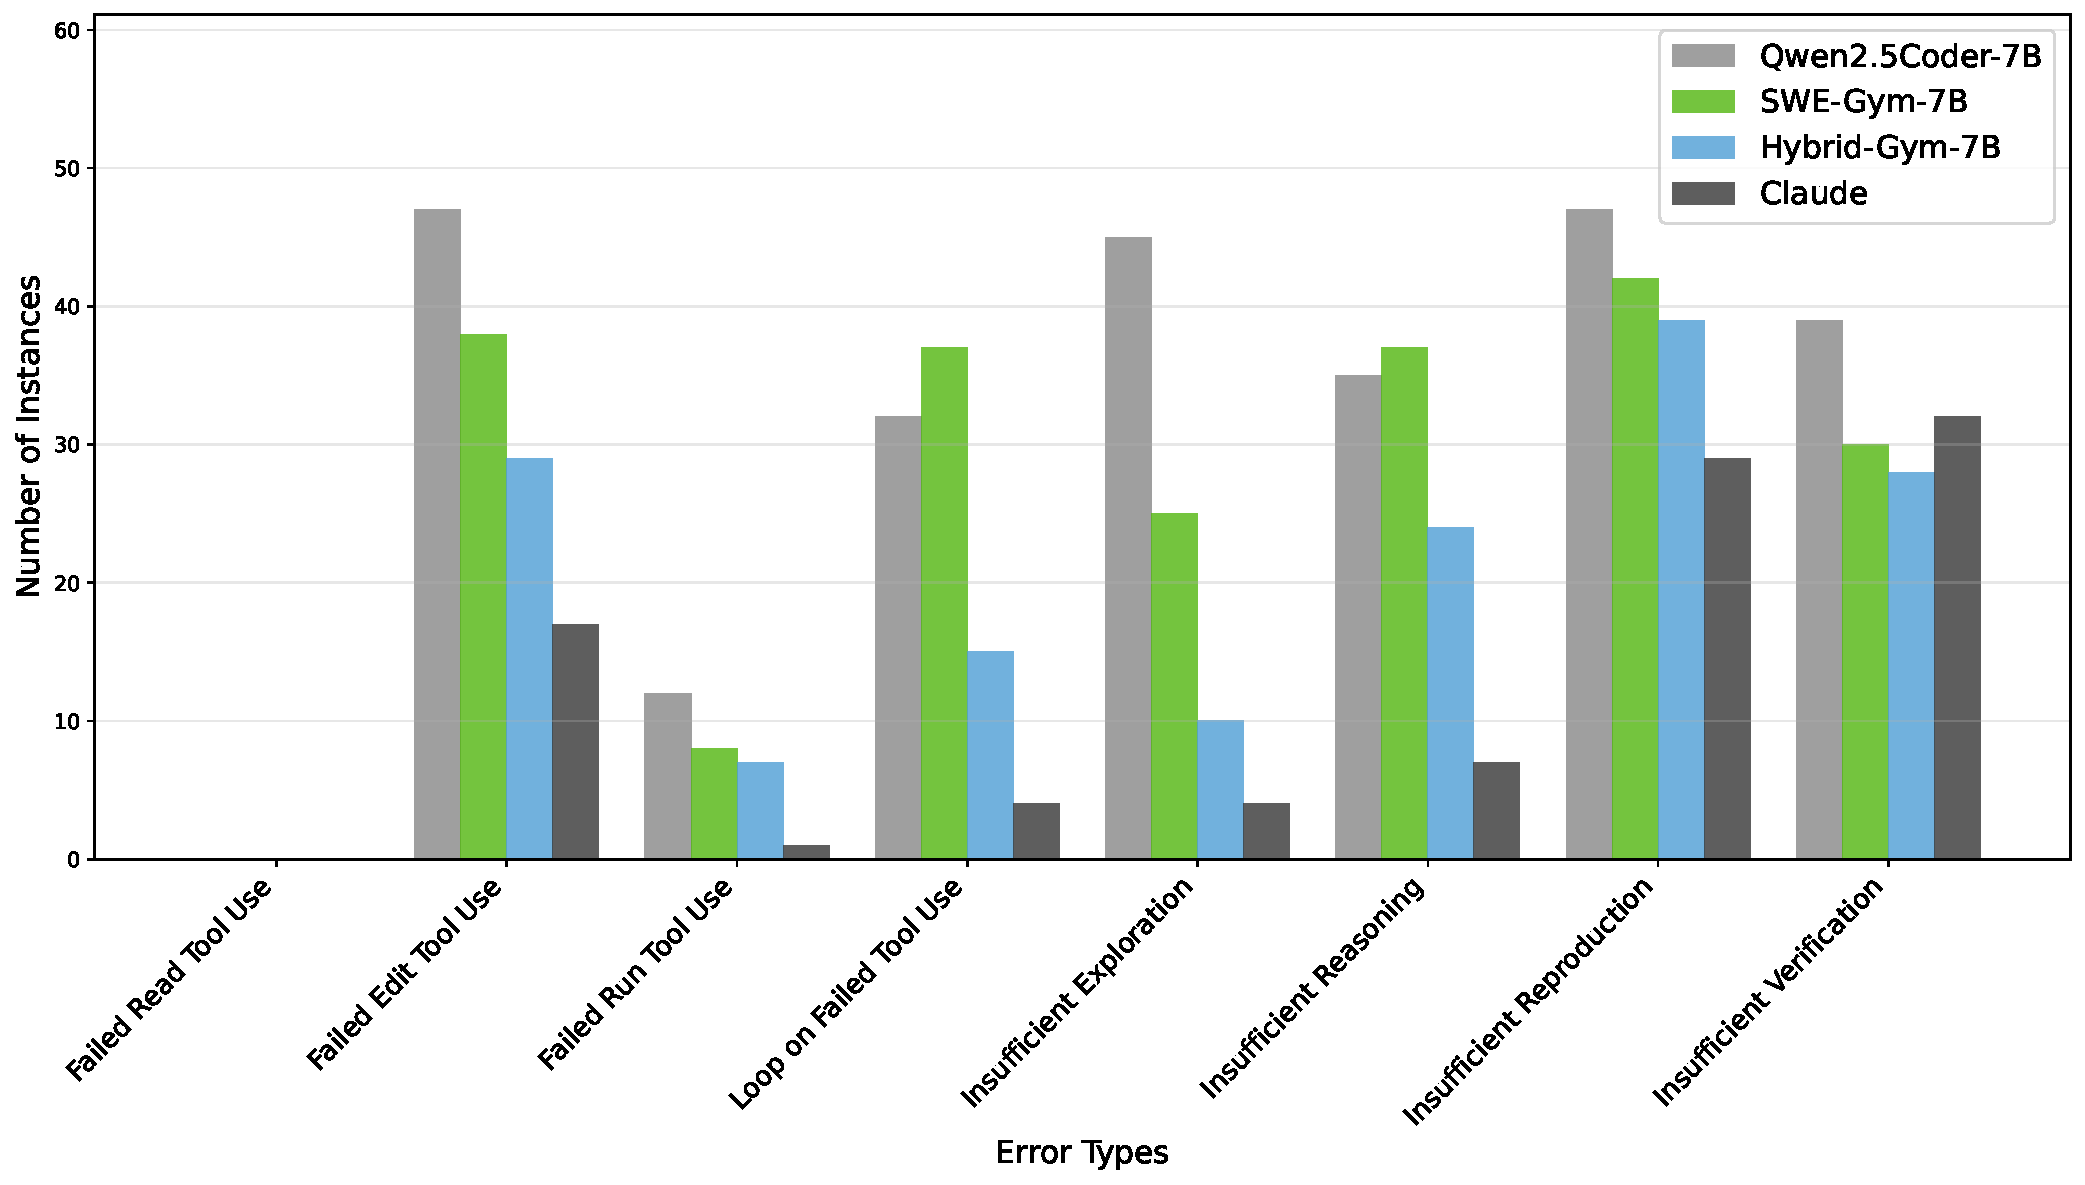
\includegraphics{HybridGym_figs/error_analysis.pdf}%
}
\caption{The error analysis of different methods on 50 instances sampled from SWE-Bench Verified.}
\label{fig:error-analysis}
\end{figure}








\section{Methodology}
\label{sec:methodology}
In this section, we first guide training task design by analyzing the commonalities shared among coding tasks and agent capabilities (\S\ref{sec:analysis-methodology}).
Based on the analysis results, we introduce a list of task design principles (\S\ref{sec:principle}) and present the four \repostmethodname tasks that satisfy all the principles (\S\ref{sec:tasks}).
Finally, we conduct a comparison between our training tasks and real-world coding tasks (\S\ref{sec:task-verification}).

\subsection{Analysis of Coding Agent Task Transferability}
\label{sec:analysis-methodology}
With the ultimate goal of designing training tasks that transfer to diverse downstream tasks, we first investigate the commonalities shared by real-world tasks by answering:
[\textbf{RQ1}] What are the commonalities of the components (i.e., high-level problem-solving steps) to complete real-world coding tasks?
[\textbf{RQ2}] What are the commonalities of the concrete actions (i.e., commands) taken by the agents?
Since effective training must target capabilities the agent has not yet learned, we also ask
[\textbf{RQ3}] What are the abilities that the agent has not learned but are required for task completion?

\start{Analysis Setup}
Following prior works~\citep{swegym,R2EGym,swe-play}, we adopt the rejection sampling finetuning setting, where we finetune Qwen2.5-Coder-7B/32B on the successful trajectories generated for the training tasks. 
We conduct the analysis based on 200 successful trajectories sampled from each task, which are generated by Claude-4.5~\cite{claude45} using OpenHands CodeAct as the agent scaffold~\cite{openhands}


\start{Task Analysis: Decomposition of Coding Tasks}
To answer \textbf{RQ1}, we first decompose general coding agent tasks into five intermediate components: reasoning, repo-exploration, execution of existing code, solution implementation, and verification. 
We then use o3-mini~\cite{o3_mini} to categorize each agent action by the component it targets.
We manually examined 20 cases and made the same categorization as o3-mini in all the cases.

Results in \autoref{tab:action-category} show that (1) The action distribution across different components is similar for the three downstream tasks, with repo-exploration accounting for the largest share.
(2) We notice that around 70\% of the actions fall into categories that do not require setting up executable repositories: reasoning, repo-exploration, and implementation.
This is notable because executable repository setup is complicated and challenging for both humans and agents~\cite{swe-smith,swe-play} and is the bottleneck of constructing scalable training datasets.
Our analysis hence suggests a key direction: training tasks that avoid executable repository setup can also be beneficial.


\start{Task Analysis: Concrete Actions Used in Coding Tasks}
To answer \textbf{RQ2}, we analyze the concrete agent tools used in each task. 
The tools built for the OpenHands agent~\cite{openhands} include bash command execution (\texttt{execute-bash}), file viewing (\texttt{view}), and file editing (\texttt{str-replace}).
Results in \autoref{tab:action-category} show that all three tools are heavily used across downstream tasks. This suggests that \emph{the agents need to learn all the tools in training.}

For the bash execution tool, we further analyze the specific commands issued by the agent. \autoref{tab:cmd-category} shows that different tasks rely on highly similar repo-exploration commands, such as grep, find, cd, and ls, suggesting that \emph{repo-exploration skills could be broadly transferable across tasks.}


\start{Agent Capability Analysis}
To answer \textbf{RQ3}, under the setting of distillation-based training, we conduct an error analysis for the untrained student model (Qwen2.5Coder-7B, \citet{qwen25coder}), the student model trained on a baseline dataset (SWE-Gym, \citet{swegym}), and the teacher model (Claude-4.5, \citet{claude45}).
We define error categories along two axes: (1) failures in the intermediate components identified in our previous analysis, and (2) failures in the use of each tool.
We then prompt an LLM to label whether each agent trajectory exhibits these failures.


\autoref{fig:error-analysis} presents the error analysis results.
We observe several error categories where the fine-tuned model’s failure rate remains far higher than the teacher model’s: insufficient repo-exploration, insufficient reasoning, and failure/loop on the file-editing tool.
This suggests that \emph{these capabilities still have substantial room for improvement.}





\subsection{Principles for Training Task Design}
\label{sec:principle}
We summarize the analysis results in \S\ref{sec:analysis-methodology} as follows:
(1) reasoning, repo-exploration, and implementation are the dominant intermediate components shared across coding-agent tasks;
(2) The concrete types of commands to complete these components are also similar across tasks; and
(3) The performance gaps between the student and teacher models are still large for the above categories and file editing.

Based on the task commonalities and the agents' capabilities, we present the following principles for training task design:

\quad [\textbf{Principle 1}] The tasks should have the same output format as the downstream tasks.
For the downstream tasks in our evaluation, the format is generating a code patch in the codebase, which requires file editing.
A counterexample for training tasks is a variant of our issue-localization task, where we only need the agent to generate the plan to resolve the issue in the message, without making any code changes.

\quad [\textbf{Principle 2}] The tasks should involve a meaningful repository-exploration phase. 
A counterexample is a script-level code generation task (e.g., HumanEval~\cite{codex}). 
Although we can still provide a repository as context by putting the solution template file inside an empty repository, it does not involve any file localization.

\quad [\textbf{Principle 3}] The tasks should require a non-trivial level of reasoning to complete. Namely, the agent must make substantive decisions, such as choosing the problem-solving strategy, generating the precise tool call arguments, and writing the code.
A counterexample is a simple string-replacement task where we provide the exact edit location and the old/new strings. The agent can succeed by a single \texttt{str-replace} call without inspecting the codebase.


With the observation that all the major components: reasoning, exploration, and implementation, do not require an executable repository, we further require the training tasks to be scalable (i.e., easy to generate new instances):

\quad [\textbf{Principle 4}] The task setup should not require substantial effort. For instance, the task should avoid installing packages for the entire repository or generating executable test files, which are challenging for both humans and agents.

In \S\ref{sec:exp}, we will show that all \repostmethodname tasks satisfy all four principles and generalize well to multiple downstream tasks.
In contrast, \S\ref{sec:controlled-exp} will show that all three counterexample tasks mentioned above do not yield effective task transfer.


\begin{table}[t]
\centering
\resizebox{0.5\linewidth}{!}{%
\begin{tabular}{lccc}
\toprule
\bf Dataset & \texttt{execute-bash} & \texttt{view} & \texttt{str-replace} \\
\midrule
Func-Localize  & 5.55  & 4.43 & 1.16 \\
Issue-Localize & 9.37  & 7.76 & 5.15 \\
Dep-Search     & 1.78  & 3.12 & 1.89 \\
Func-Gen       & 0.53  & 1.75 & 1.47 \\
\midrule
SWE-Bench      & 10.65 & 6.88 & 3.65 \\
SWT-Bench      & 16.54 & 6.09 & 5.16 \\
Commit-0       & 18.40 & 21.20 & 36.40 \\
\bottomrule
\end{tabular}%
}
\caption{The average number of OpenHands tools called in each trajectory.}
\label{tab:openhands-tool-distribution}
\end{table}

\begin{table}[t]
\centering
\resizebox{\linewidth}{!}{%
\begin{tabular}{lcccccccc}
\toprule
\multirow{2}{*}{\bf Model} &
\multicolumn{2}{c}{\bf Func-Localize} &
\multicolumn{2}{c}{\bf Issue-Localize} &
\multicolumn{2}{c}{\bf Dep-Search} &
\multicolumn{2}{c}{\bf Func-Gen} \\
\cmidrule(lr){2-3}\cmidrule(lr){4-5}\cmidrule(lr){6-7}\cmidrule(lr){8-9}
& Success \% & Non-Empty \% & Success \% & Non-Empty \% & Success \% & Non-Empty \% & Success \% & Non-Empty \% \\
\midrule
Qwen2.5Coder-7B   & 0.0\%  & 50.0\% & 3.3\%  & 16.7\% & 6.7\%  & 60.0\%  & 5.0\%  & 70.0\% \\
Qwen2.5Coder-32B  & 40.0\% & 95.0\% & 33.3\% & 83.3\% & 56.7\% & 86.7\%  & 25.0\% & 95.0\% \\
\midrule
Claude-4.5        & 70.0\% & 100.0\% & 63.3\% & 100.0\% & 80.0\% & 100.0\% & 50.0\% & 100.0\% \\
\bottomrule
\end{tabular}%
}
\caption{Performance of the student and teacher models on a subset of instances sampled from each training task.}
\label{tab:distillation-sanity-check}
\end{table}


\subsection{\repostmethodname Tasks}
\label{sec:tasks}

In this section, we introduce four \repostmethodname tasks that satisfy all the principles above.
% We provide the prompt for each task in Appendix \ref{app:data-construction}.

\start{Function Localization}
To boost repository exploration (principle 2), we design a task to localize a function in the entire codebase:
given a short description, the agent needs to identify the corresponding function in the codebase.
To satisfy Principle 1, which requires generating a code patch as the outcome, we require the agent to write a docstring containing the fix plan. 
We evaluate the task by checking whether a docstring is added for the correct function.
This task requires substantial reasoning (principle 3), as the agent needs to understand the code content and conduct an effective and targeted search over the entire repository, which contains 2,925 functions on average in our training set.

\start{Issue Localization}
Function localization aims to locate the code based on the description, and issue localization locates the problematic code based on an issue.
Given a GitHub issue, the task is to locate the relevant code in the repository and leave a comment containing a plan to fix the issue.
We evaluate the task by checking whether a comment is generated in the same file where the actual fix is located. 

Compared to the issue-solving task used in most prior work, constructing issue localization data does not need test execution for evaluation and can be instantiated from arbitrary GitHub issues.
However, it still requires reasoning effort on analyzing the issue, exploring the repository, planning the fix, and making successful file-editing actions.

\start{Dependency Search}
We have the third task that targets code localization, which requires file-editing, repo-exploration, and reasoning: given a function, the agent must identify all functions or classes it directly calls.
Similar to the above two tasks, we require adding comments to all these dependent modules.
To obtain the ground truth, we adopt \texttt{Jedi}, a static Python analysis tool, to resolve imported names to their defining modules.
Solving this task requires the agent to locate the target function, extract the referenced names, resolve each name to the correct module, and successfully edit the relevant files.
This is non-trivial because a codebase may contain multiple modules with the same name, and only one corresponds to the actual call.

\start{Function Generation}
Beyond the localization tasks that only aim to generate comments, we design the function generation task that requires actual code generation. 
Given a function in a codebase, we use an LLM to generate a description of its functionality.
Then we remove the function body and ask the agent to re-implement it.
To evaluate the implementation with test cases while avoiding repository installation, we adapt the RepoST~\cite{repost} method to the coding agent setting, which extracts the target function and its dependencies to a separate script and generates tests.

Here we highlight that generating \emph{executable test scripts} is substantially easier and more cost-efficient than setting up \emph{executable repositories}.
To execute the test script, we only need to install the packages needed by the extracted function and its dependencies (2.1 packages on average), while installing the entire repository requires 26.5 packages on average.
Furthermore, compared to \emph{generating a new test file} that requires understanding the repository structure and resolving relative imports, it is substantially easier to \emph{produce tests for a separate script}, which only requires seq-to-seq generation, without any agentic frameworks, making the setup process cost-efficient.

We emphasize that \repostmethodname is not limited to the specific tasks introduced here: other task designs may also satisfy our principles.
It is also possible to construct variants of our tasks, such as localizing multiple functions, or finding the empty function before generating the function body. We leave the exploration to future works. 

\begin{table}[t]
    \centering
  \resizebox{0.7\linewidth}{!}{%
    \begin{tabular}{lccccc}
      \toprule
      \bf Dataset & \bf \# Trajs & \bf \# Repos & \bf Avg Steps & \bf \# Images & \bf Cost \\
      \midrule
      SWE-Gym   & 491   & 11  & 40.2 & 2.4k & unknown \\
      R2E-Gym   & 3,321 & 10  & 33.2 & 4.5k & unknown \\
      SWE-Smith & 5,016 & 128 & 26.7 & 128  & 2.32\textcent \\
      SWE-Play  & 704   & 28  & 72.9 & 28   & unknown \\
      \midrule
      \repostmethodname & 4,470 & 762 & 39.1 & 2 & 0.07\textcent \\
      \hdashline
      \quad Func-Localize  & 1,438 & 226 & 29.0 & 1 & 0.02\textcent \\
      \quad Issue-Localize & 1,978 & 263 & 52.4 & 1 & 0.00\textcent \\
      \quad Dep-Search     & 502   & 120 & 26.9 & 1 & 0.00\textcent \\
      \quad Func-Gen       & 552 & 306 & 28.6 & 1 & 0.56\textcent \\
      \bottomrule
    \end{tabular}%
  }
  \caption{Statistics of \repostmethodname and its subsets.
  Following SWE-Smith, we report the average per-instance cost of setting up the training environment for rollout.
  Compared to existing datasets, \repostmethodname covers more repositories and requires only 2 docker images to build all training instances.}
  \label{tab:stat}
\end{table}

\begin{figure}[t]
    \centering
    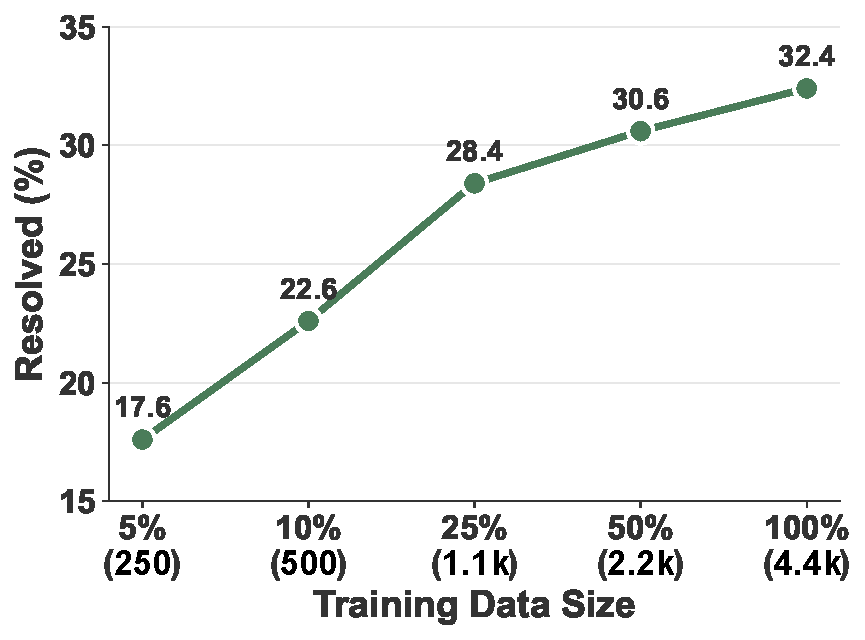
\includegraphics[width=0.6\linewidth]{HybridGym_figs/fig_scaling_law_v2.pdf}
  \caption{Scaling law analysis. Performance on SWE-bench Verified improves consistently as training data size increases from around 5\% (250 trajectories) to 100\% (4.4k trajectories).}
  \label{fig:scaling}
\end{figure}



\subsection{Verification of \repostmethodname Tasks}
\label{sec:task-verification}
In this section, we verify that our training tasks share commonalities with real-world tasks and remain challenging for the student models we use: Qwen2.5Coder 7B and 32B.

\start{\repostmethodname tasks cover the majority of intermediate components in multiple real-world tasks}
As shown in \autoref{tab:action-category}, all the training tasks cover reasoning, repo-exploration, and implementation, and the function-generation task additionally includes solution verification.
We note that although our training tasks do not explicitly include executing existing code, it typically accounts for only a small fraction of an agent's trajectory.

\start{\repostmethodname trajectories contain similar actions with real-world tasks}
As shown in \autoref{tab:cmd-category}, the training tasks use a similar set of bash commands for repo-exploration as the real-world coding tasks.
Similarly, \autoref{tab:openhands-tool-distribution} shows that the training tasks cover the full set of OpenHands tools used in downstream tasks.
Together, these results suggest that both the high-level problem-solving components and the concrete actions that achieve them can transfer across \repostmethodname tasks and downstream tasks.


\start{\repostmethodname tasks are still challenging for models without finetuning}
Under the setting of distillation learning, a training task is useful only if there is a performance gap between the student and teacher models
As a sanity check, before generating training data, we sample 20-30 instances from each task and evaluate the teacher model (claude-4.5-Sonnet) and student models (Qwen2.5Coder, 7B and 32B).

\autoref{tab:distillation-sanity-check} show that Claude-4.5 achieves substantially higher success rates than Qwen2.5Coder-32B on all four tasks, with gaps ranging from 23.3\% to 30.0\%. This confirms that all tasks provide sufficient room for effective distillation.







\section{Results}
\label{sec:exp}

\subsection{Experimental Setup}
\start{Statistics of \repostmethodname}
\autoref{tab:stat} presents the statistics of \repostmethodname and existing datasets. 
Based on the scalable training tasks, we collect 4.4k trajectories from 762 repositories using only two Docker images.
The environment construction cost is only 0.07\textcent per example, which is 16× lower than SWE-Smith~\cite{swe-smith}.
Trajectory lengths vary by task, ranging from 26.9 to 52.4 agent steps, which are comparable to the issue-solving trajectories in prior datasets, suggesting that our tasks retain a meaningful level of complexity.
The trajectories are obtained from the combination of Claude-4.5~\cite{claude45}, Claude-3.7~\cite{claude37}, and Qwen3-235b~\cite{qwen3}.
% We provide dataset details in Appendix~\ref{app:data-construction}.


\begin{table*}[t]
\centering

\resizebox{\textwidth}{!}{%
\begin{tabular}{c@{\hspace{2pt}}c@{\hspace{2pt}}c@{\hspace{2pt}}c l ccc cc c}
\toprule
\multicolumn{4}{c}{ \multirow{2}{*}{\bf Training Tasks} } &
\multirow{2}{*}{\bf Training Dataset} 
& \multicolumn{3}{c}{Issue Solving (swe)} 
& \multicolumn{2}{c}{Test Generation (swt)} 
& \multicolumn{1}{c}{Library Build (cmt)}\\
& & & &
& \multicolumn{3}{c}{\bf SWE-bench Verified} 
& \multicolumn{2}{c}{\bf SWT-Bench Lite \& Verified} 
& \multicolumn{1}{c}{\bf Commit-0 Lite} \\
\cmidrule(lr){1-4}
\cmidrule(lr){6-8}\cmidrule(lr){9-10}\cmidrule(lr){11-11}
swe & swt & cmt & syn
& & Resolved \% & Localized \% & Non-Loop \%
& Lite Resolved & Verified Resolved
& Resolved \% \\
\midrule

\sdlrow & \multicolumn{10}{c}{\textit{Base Model: Qwen2.5Coder-7B}} \\
& & & 
& (\textit{base}) Qwen2.5Coder-7B    & 1.8  & 4.4 & 60.4 & 0.72 & 0.23 & 4.80 \\

& & & \cmark
& SWE-Play-general & 8.6~{\textcolor{treegreen}{+6.8}} & 49.2~{\textcolor{treegreen}{+44.8}} & 93.4~{\textcolor{treegreen}{+33.0}} & 2.54~{\textcolor{treegreen}{+1.82}} & 1.62~{\textcolor{treegreen}{+1.39}} & 9.25~{\textcolor{treegreen}{+4.45}} \\

\cmark & & &
& SWE-Gym          & \dlcell 10.6~{\textcolor{treegreen}{+8.8}}  & \dlcell 48.2~{\textcolor{treegreen}{+43.8}} & \dlcell 79.0~{\textcolor{treegreen}{+18.6}} & 1.45~{\textcolor{treegreen}{+0.73}} & 0.69~{\textcolor{treegreen}{+0.46}}  & 8.61~{\textcolor{treegreen}{+3.81}} \\

\cmark & & &
& R2E-Gym          & \dlcell \bf 19.0~{\textcolor{treegreen}{+17.2}} & \dlcell \textemdash & \dlcell \textemdash  & 0.72~{\textcolor{gray}{+0.00}}      & 0.46~{\textcolor{treegreen}{+0.23}}  & 9.25~{\textcolor{treegreen}{+4.45}} \\

\cmark & & &
& SWE-smith        & \dlcell 15.2~{\textcolor{treegreen}{+13.4}} & \dlcell \textemdash & \dlcell \textemdash  & 0.00~{\textcolor{red}{-0.72}}     & 0.00~{\textcolor{red}{-0.23}} & 9.32~{\textcolor{treegreen}{+4.52}} \\

\cmark & \cmark & \cmark & \cmark
& SWE-Play & \dlcell 17.0~{\textcolor{treegreen}{+15.2}} & \dlcell 60.4~{\textcolor{treegreen}{+56.0}} & \dlcell 91.2~{\textcolor{treegreen}{+30.8}} & \dlcell 3.26~{\textcolor{treegreen}{+2.54}} & \dlcell 3.00~{\textcolor{treegreen}{+2.77}} & \dlcell 10.42~{\textcolor{treegreen}{+5.62}} \\
\midrule

& & & \cmark
& \textbf{\repostmethodname}      & 15.0~{\textcolor{treegreen}{+13.2}} & \bf 62.4~{\textcolor{treegreen}{+58.0}} & \bf 97.6~{\textcolor{treegreen}{+37.2}} & 2.90~{\textcolor{treegreen}{+2.18}} & 2.54~{\textcolor{treegreen}{+2.31}} & 10.54~{\textcolor{treegreen}{+5.74}} \\

\cmark & \cmark & \cmark & \cmark
& \textbf{\repostmethodname} + SWE-Play
& \dlcell 17.6~{\textcolor{treegreen}{+15.8}} & \dlcell 58.6~{\textcolor{treegreen}{+54.2}} & \dlcell 97.2~{\textcolor{treegreen}{+36.8}} & \dlcell \bf 5.07~{\textcolor{treegreen}{+4.35}} & \dlcell \bf 4.39~{\textcolor{treegreen}{+4.16}} & \dlcell \bf 11.02~{\textcolor{treegreen}{+6.22}} \\
\midrule

\sdlrow & \multicolumn{10}{c}{\textit{Base Model: Qwen2.5Coder-32B}} \\
% \textemdash & \textemdash & \textemdash & \textemdash
& & & 
& (\textit{base}) Qwen2.5Coder-32B    & 7.0  & 45.6 & 70.6 & 9.42 & 9.01 & 8.34 \\

\cmark & & &
& SWE-Gym          & \dlcell 20.6~{\textcolor{treegreen}{+13.6}} & \dlcell 57.8~{\textcolor{treegreen}{+12.2}} & \dlcell 76.2~{\textcolor{treegreen}{+5.6}} & 3.26~{\textcolor{red}{-6.16}} & 2.77~{\textcolor{red}{-6.24}} & 9.58~{\textcolor{treegreen}{+1.24}} \\

\cmark & & &
& R2E-Gym          & \dlcell 34.4~{\textcolor{treegreen}{+27.4}} & \dlcell \textemdash & \dlcell \textemdash & 3.26~{\textcolor{red}{-6.16}} & 4.39~{\textcolor{red}{-4.62}} & 11.56~{\textcolor{treegreen}{+3.22}} \\

\cmark & & &
& SWE-smith        & \dlcell \bf 40.2~{\textcolor{treegreen}{+33.2}} & \dlcell \textemdash & \dlcell \textemdash & 13.77~{\textcolor{treegreen}{+4.35}} & 10.62~{\textcolor{treegreen}{+1.61}} & 12.38~{\textcolor{treegreen}{+4.04}} \\

\cmark & \cmark & \cmark & \cmark
& SWE-Play     & \dlcell 31.2~{\textcolor{treegreen}{+24.2}} & \dlcell 73.4~{\textcolor{treegreen}{+27.8}} & \dlcell 85.2~{\textcolor{treegreen}{+14.6}} & \dlcell 18.12~{\textcolor{treegreen}{+8.70}} & \dlcell 16.17~{\textcolor{treegreen}{+7.16}} & \dlcell 13.95~{\textcolor{treegreen}{+5.61}} \\
\midrule

& & & \cmark
& \textbf{\repostmethodname}      & 32.4~{\textcolor{treegreen}{+25.4}} & \bf 75.4~{\textcolor{treegreen}{+29.8}} & 98.2~{\textcolor{treegreen}{+27.6}} & 17.03~{\textcolor{treegreen}{+7.61}} & 16.86~{\textcolor{treegreen}{+7.85}} & 13.45~{\textcolor{treegreen}{+5.11}} \\

\cmark & \cmark & \cmark & \cmark
& \textbf{\repostmethodname} + SWE-Play
& \dlcell 33.6~{\textcolor{treegreen}{+26.6}} 
& \dlcell 75.2~{\textcolor{treegreen}{+29.6}} 
& \dlcell \bf 99.2~{\textcolor{treegreen}{+28.6}} 
& \dlcell \bf 20.29~{\textcolor{treegreen}{+10.87}}
& \dlcell \bf 21.02~{\textcolor{treegreen}{+12.01}}
& \dlcell \bf 15.52~{\textcolor{treegreen}{+7.18}}
\\
\bottomrule
\end{tabular}%
}


\caption{Results on three real-world coding tasks.
We show whether the datasets contain swe, swt, cmt, or synthetic tasks (syn) in training.
Results with a white background are \textbf{task transfer} results.
Results with a light grey background are trained with in-domain tasks.
We highlight the best result for each dataset and show the relative \textcolor{treegreen}{gain} and \textcolor{red}{loss} compared to the base model, Qwen2.5Coder.
\repostmethodname achieves strong task transfer performances across all three benchmarks and further improves in-domain datasets (e.g., SWE-Play).
}
\label{tab:main}
\end{table*}










\start{Evaluation Datasets and Metrics}
We follow prior work~\cite{swe-play} and report the resolved rates on SWE-Bench Verified~\cite{swebench}, SWT-Bench Lite/Verified~\cite{swt-bench}, and Commit-0~\cite{commit0}.
On SWE-Bench, we additionally report the localized rate: the percentage of code patches applied to the correct file, and the non-loop rate: the percentage of trajectories without any ``loops'', which is defined as repeating the same action three times consecutively~\cite{swegym}.



\subsection{Main Results}
\start{\repostmethodname Shows Strong Task Transfer Performance}
Results in \autoref{tab:main} show that \repostmethodname delivers strong task generalization performance across all three benchmarks. Relative to the base 32B model, it improves performance by 25.40 \% / 7.85 \% / 5.11 \% on the three tasks, outperforming all existing task transfer training datasets.
Notably, without training on the downstream tasks, \repostmethodname matches or even exceeds in-domain training. For example, SWE-Play-32B reaches 31.2 \% / 16.17 \% on SWE-Bench Verified / SWT-Bench Verified, whereas \repostmethodname-32B achieves 32.4 \% / 16.86 \%. 
This suggest that our tasks capture the commonality shared among general coding agent tasks and transfer effectively across all three downstream tasks.
These results are especially compelling because \repostmethodname requires substantially less effort to build new training instances than prior datasets (e.g., as shown in \autoref{tab:stat}, SWE-Smith requires 128 docker images and costs 2.32\textcent per example, while \repostmethodname is only built with 2 images and an average cost of 0.07\textcent).


\start{\repostmethodname Improves In-Domain Training Datasets}
\autoref{tab:main} further shows that we can further improve in-domain datasets by combining with \repostmethodname. For instance, we improve SWE-Play by 2.40\% / 4.85\% / 1.57\% on SWE-Bench Verified / SWT-Bench Verified / Commit-0 Lite.
The gains from mixing \repostmethodname with in-domain data suggest that the two sources are complementary. \repostmethodname primarily teaches general agent skills (e.g., reasoning, repo-exploration, and reliable tool use), while in-domain data contributes task-specific behaviors (e.g., generating tests and building libraries from scratch). Combining them both leads to additive improvements.

\begin{table}[t]
\centering
\small
\resizebox{0.7\columnwidth}{!}{%
\begin{tabular}{l ccc}
\toprule
\bf Training Tasks & \bf SWE-Bench & \bf SWT-Bench & \bf Commit-0 \\
(\# Instances) & Resolved \% & Resolved \% & Resolved \% \\
\midrule
Qwen2.5Coder-7B & 1.8 & 0.23 & 4.80 \\
+ Issue-Solving (491) & \dlcell 10.6~{\scriptsize\textcolor{treegreen}{+8.8}} & 0.69~{\scriptsize\textcolor{treegreen}{+0.46}} & 8.61~{\scriptsize\textcolor{treegreen}{+3.81}} \\
\midrule
+ Func-Localize (500) & 12.8~{\scriptsize\textcolor{treegreen}{+11.0}} & \bf 3.00~{\scriptsize\textcolor{treegreen}{+2.77}} & 8.74~{\scriptsize\textcolor{treegreen}{+3.94}} \\
+ Issue-Localize (500) & 9.6~{\scriptsize\textcolor{treegreen}{+7.8}} & 2.31~{\scriptsize\textcolor{treegreen}{+2.08}} & 9.09~{\scriptsize\textcolor{treegreen}{+4.29}} \\
+ Dep-Search (500) & 6.4~{\scriptsize\textcolor{treegreen}{+4.6}} & 2.31~{\scriptsize\textcolor{treegreen}{+2.08}} & 9.25~{\scriptsize\textcolor{treegreen}{+4.45}} \\
+ Func-Gen (500) & 7.8~{\scriptsize\textcolor{treegreen}{+6.0}} & 2.54~{\scriptsize\textcolor{treegreen}{+2.31}} & 9.25~{\scriptsize\textcolor{treegreen}{+4.45}} \\
% \midrule
\hdashline
\addlinespace[0.5ex]
+ \textbf{\repostmethodname}-full & \bf 15.0~{\scriptsize\textcolor{treegreen}{+13.2}} & 2.54~{\scriptsize\textcolor{treegreen}{+2.31}} & \bf 10.54~{\scriptsize\textcolor{treegreen}{+5.74}} \\

\bottomrule
\end{tabular}%
}
\caption{Performance of training Qwen2.5Coder-7B on each of the \repostmethodname tasks and the issue-solving task. We sample 500 instances from each of our tasks.
Even without finetuning on issue-solving, function localization achieves a larger performance gain than SWE-Gym, which has 491 issue-solving instances.
We report the resolved rates on SWE-Bench Verified, SWT-Bench Verified, and Commit-0 Lite. 
}
\label{tab:single-task}
\end{table}



\subsection{Detailed Results}

\start{Training on Individual Tasks}
To assess the contribution of each task, we sample 500 instances per task and train the model on each subset separately. This training size is comparable to the SWE-Gym issue-solving dataset, which contains 491 examples. As shown in \autoref{tab:single-task}, each task yields a substantial improvement over the base model, with gains ranging from 4.6\% to 11.0\%. The tasks emphasize different capabilities (e.g., function localization performs best on SWE-Bench but worst on Commit-0), while the full \repostmethodname dataset—combining all four tasks—achieves the strongest overall performance.

Notably, at similar training scales, the function-localization and issue-localization tasks provide gains that are comparable to, or even exceed, in-domain training. For example, SWE-Gym achieves a 10.6\% resolved rate and a 48.2\% localized rate, whereas Func-Localize (500) reaches 12.8\% and 53.6\%. A possible explanation is that localization trajectories devote more steps to repo-exploration than issue-solving, which is one of the agent’s primary bottlenecks.



\start{Scaling Law Analysis}
As shown in \autoref{fig:scaling}, we train the 32B model on progressively larger subsets of \repostmethodname, where we proportionally sample training instances from each task. 
The performance continues to improve as the dataset grows and still shows improvements when we have 4.4k training trajectories.
The results suggest the advantage of constructing highly scalable training datasets.






\begin{figure*}[t]
\centering
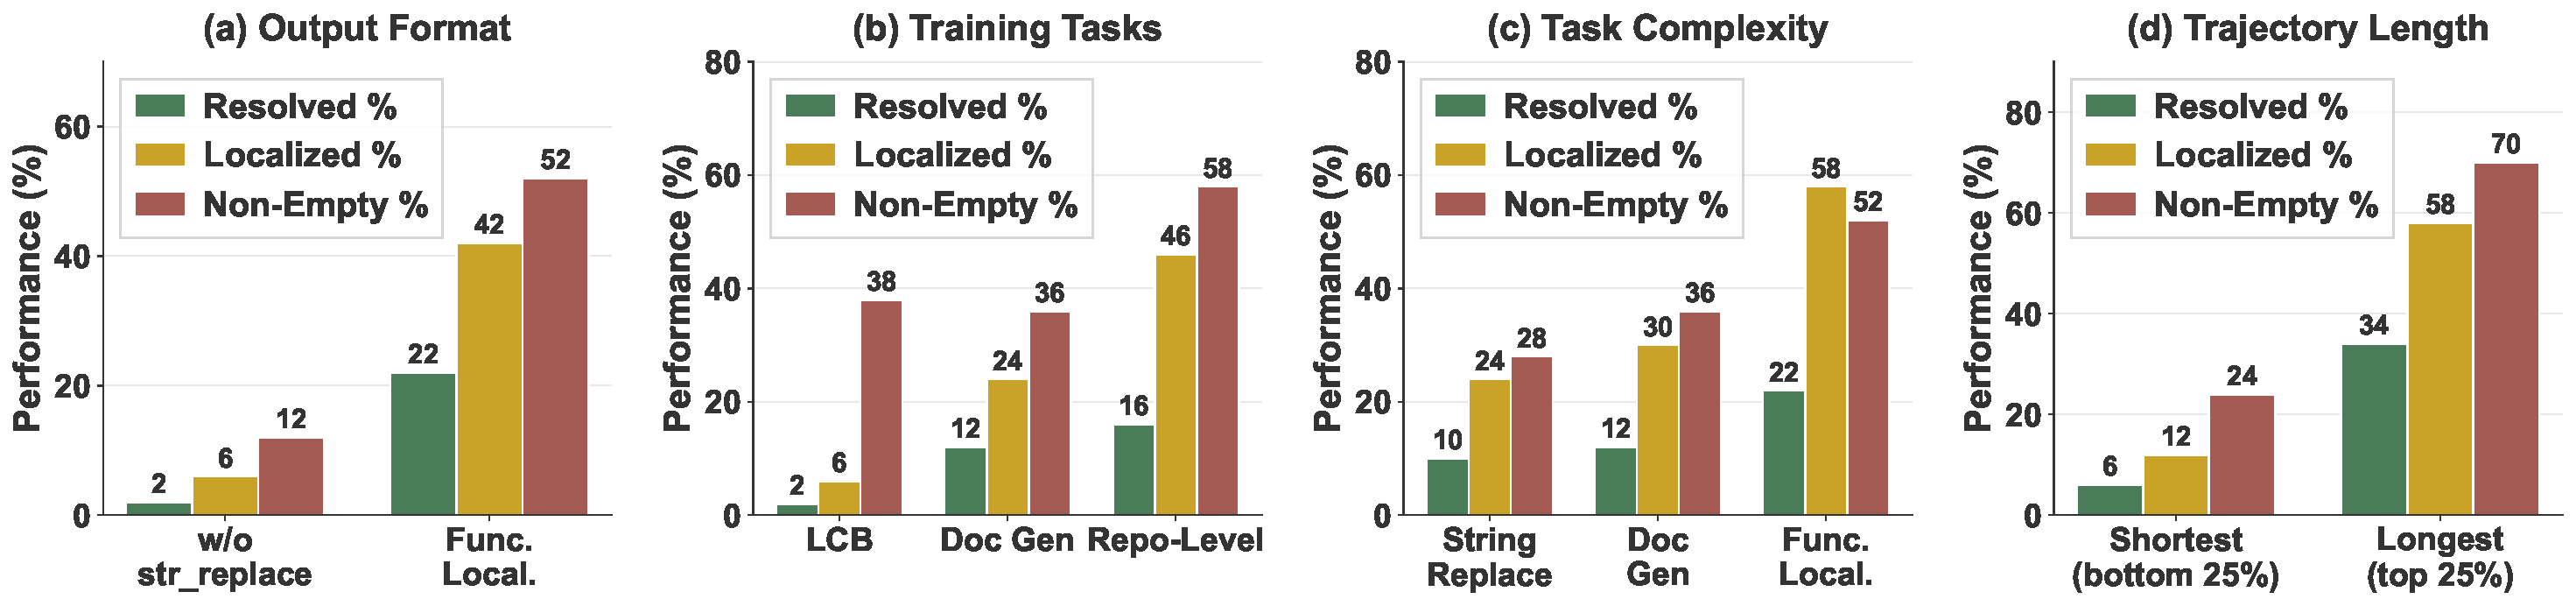
\includegraphics[width=\textwidth]{HybridGym_figs/fig_combined_bcde.pdf}
\caption{Controlled experiments on training data characteristics.
(a)~\textbf{Output Format:} Removing the file editing actions (\texttt{str\_replace}) from function localization trajectories causes a large drop in SWE-bench resolution rate.
(b)~\textbf{Repo-Exploration:} script-level code generation (LCB) does not effectively transfer to repo-level issue-solving and even underperforms documentation generation, a simple repo-level task.
(c)~\textbf{Task Complexity:} Transfer improves as training tasks become more complex.
(d)~\textbf{Trajectory Complexity:} With a fixed data size, training on longer (more agent steps) trajectories substantially improves downstream performance.}
\label{fig:ablation}
\end{figure*}







\section{Analysis of Task Transferability}
\label{sec:controlled-exp}

We have established in \S\ref{sec:exp} that the particular tasks included in \repostmethodname are effective for task generalization across diverse real-world coding benchmarks. 
In this section, we investigate: \textbf{what properties of these trajectories enable task transfer?}
To answer this, we run controlled ablations that systematically modify trajectory structure and measure the resulting changes in performance.

As the ablations require repeated evaluation across many variations, we keep the analyses computationally tractable by evaluating on an easier subset of SWE-bench examples (denoted as ``Easy 50''), which are solvable by Deepseek-v3, a strong reference model \cite{deepseekv3}. 


\subsection{Output Format Must Match Downstream Tasks}
While our tasks are designed around higher level tasks such as function localization and generation, we also find that \textit{how} these behaviors are expressed in the training trajectories matters. Specifically, as stated in [\textbf{Principle 1}] in \S\ref{sec:methodology}, we find that the output format of the tasks is a crucial factor.

All three downstream tasks in our experiments require the agent to generate a code patch as the output. To isolate the role of output format, we conduct a minimal ablation on our function localization task: instead of requiring the model to generate a comment in the codebase containing the fix plan, we simply ask it to generate the plan in a message.
We accordingly modify the training trajectories by removing the \texttt{str\_replace} actions for writing comments and adding the fix plan in the final message generated by the agent.

As shown in \autoref{fig:ablation}, performance on SWE-bench collapses when we remove the string replacement actions. These results suggest that for coding agent tasks, the production of \textbf{patch-like outputs} is not a superficial formatting choice but a crucial skill that the agent needs to learn. 


\subsection{Script-level Agentic Tasks Do NOT Generalize to Repo-level Tasks}
\label{sec:ablation_lcb}
We then validate [\textbf{Principle 2}], which requires the training tasks to have a repo-exploration stage. 
To test this, we implement a script-level task, LiveCodeBench (LCB) \cite{livecodebench}, which primarily evaluates function generation in a single file. 
We contrast it with two repo-level tasks: 
(1) the repo-level function generation task we use in \repostmethodname (introduced in \S\ref{sec:methodology}), and 
(2) documentation generation, which requires the agent to generate the docstring for a given function.
For fair comparison, we wrap the coding template and test script in LCB in a dummy repository so that the model interacts with the same harness and tool API. 


\autoref{fig:ablation} shows that despite having the wrapper to make LCB superficially a repo-level task, LCB is not effective for transfer to SWE-bench. 
This negative result suggests that repository-level generalization requires more than superficial ``agentic formatting.'' 
In particular, repo-level tasks induce behaviors that are largely absent from script-level problems: identifying and navigating relevant files, grounding edits in existing codebase structure, and producing concrete patch-like modifications that apply cleanly in context. 



\begin{figure}[t]
\centering
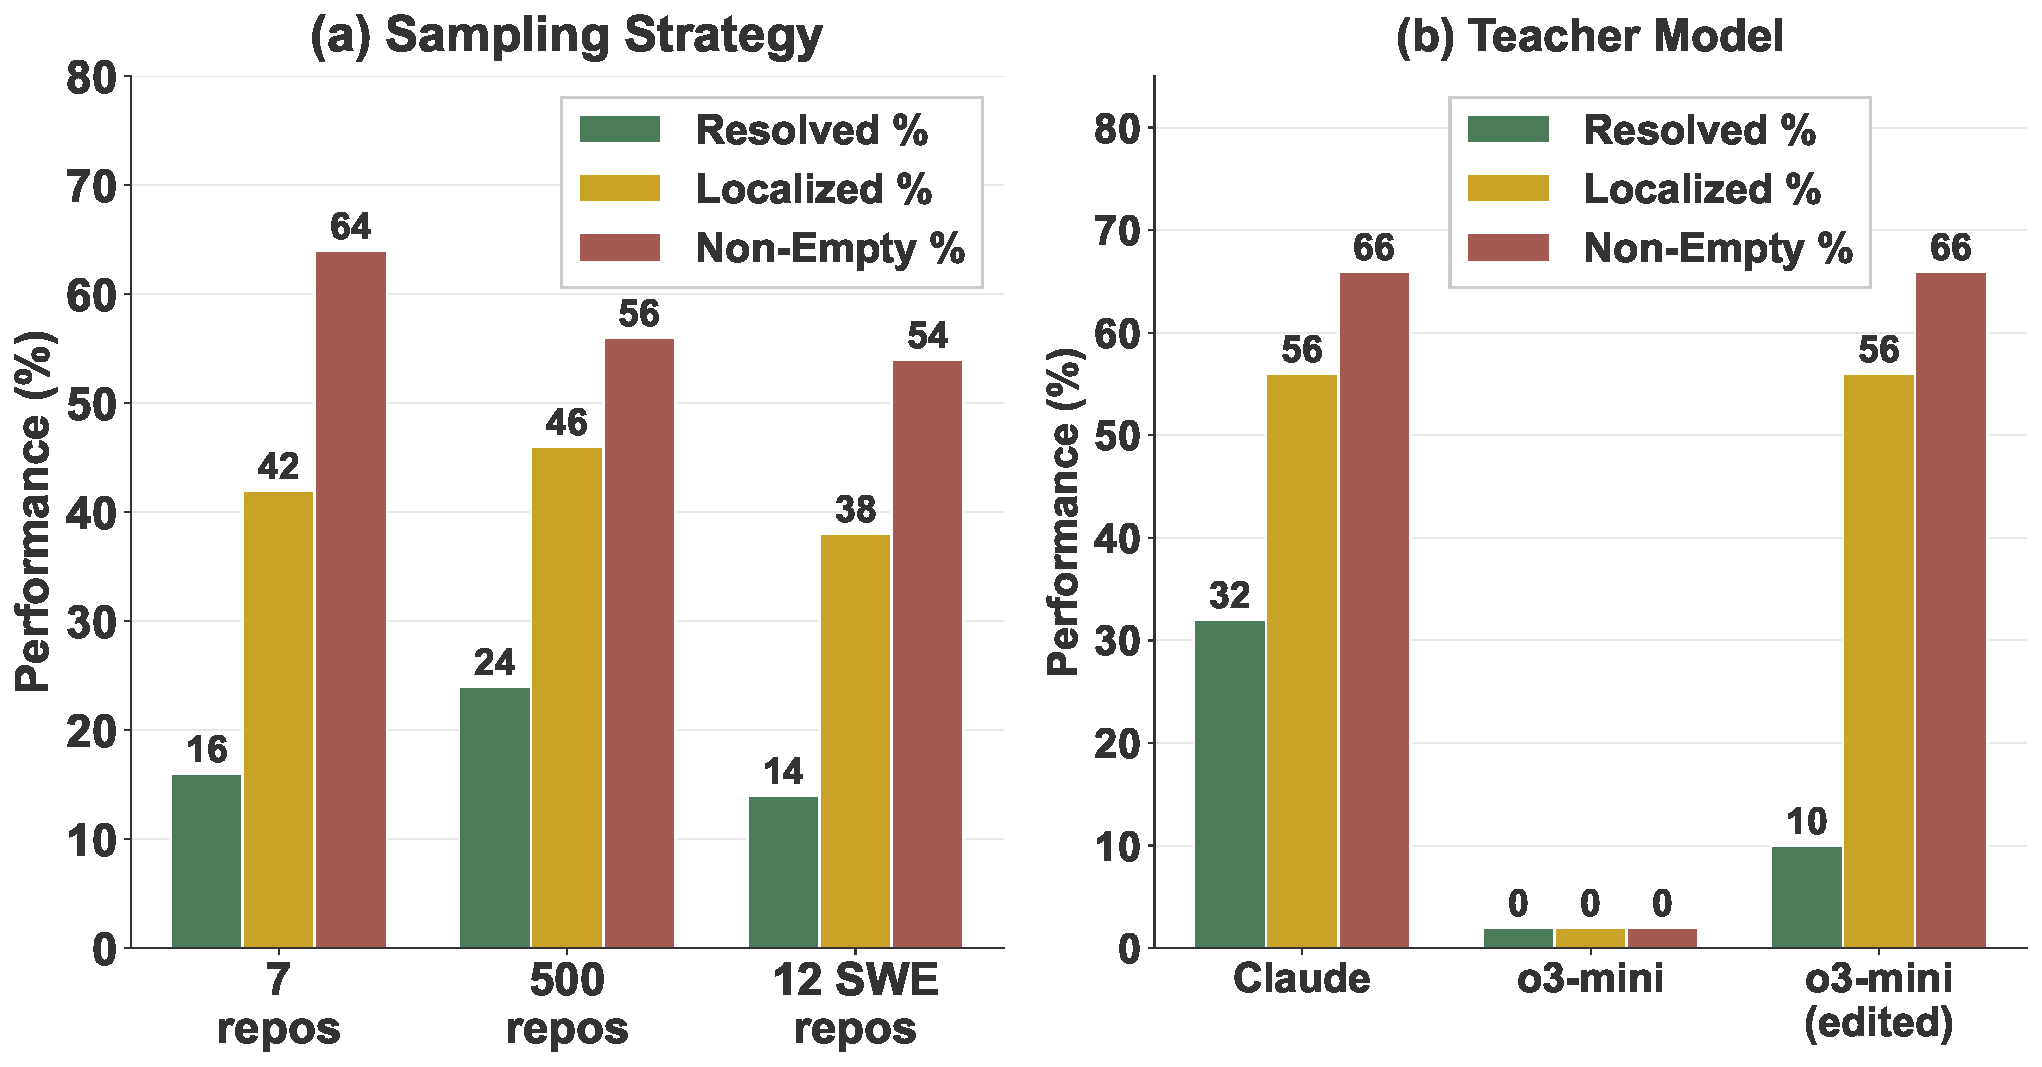
\includegraphics[width=0.7\columnwidth]{HybridGym_figs/fig_sampling_teacher_combined.pdf}
\caption{Effect of teacher model and data selection. (a) Effect of \textbf{sampling strategy} at fixed training budget. Repository diversity improves training but using the same repositories as in evaluation does not. 
(b) training on issue localization trajectories with different \textbf{teacher models}. o3-mini (edited) indicates the same set of trajectories as o3-mini, but with text and action steps combined. 
}
\label{fig:sampling_teacher}
\end{figure}

\subsection{Task and Trajectory Complexity Matters}
\label{sec:ablation_complexity}
After identifying reasoning and planning as a crucial component in coding tasks in \S\ref{sec:methodology}, we derive [\textbf{Principle 3}] that requires the task to involve a non-trivial level of reasoning.
Here, we examine whether task generalizability improves as training supervision more closely matches the multi-step, tool-mediated interaction patterns required for coding tasks. 

We first examine tasks with ascending complexity: (1) single-shot string-replacement edits in which the task is to refactor a function by simply renaming it without replacing other usages of it, (2) documentation generation for a fixed function (as in $\S\ref{sec:ablation_lcb}$), and (3) the function localization task, which requires more complex reasoning than the previous two tasks.
We see in \autoref{fig:ablation} that as tasks become more complex and interaction-heavy, downstream SWE-bench performance improves, and models are substantially more likely to produce non-empty patches.


To isolate complexity effects from task identity, we also investigate the effect of \emph{trajectory complexity}, which is operationalized as the number of agent actions (tool calls and intermediate components) taken in successful trajectories.
We pool trajectories from our repo-level task mixture and partition them by length, selecting the shortest and longest quartiles (25\% each). 
As shown in \autoref{fig:ablation}, although the training sizes are the same, training on longer trajectories yields a large improvement in SWE-bench resolution rate, alongside a sharp reduction in empty generations. These results suggest that trajectory complexity is an important driver of task performance.



\subsection{Even Successful Trajectories of the Same Task Instances may have Different Impact}
In addition to training task design, we observe that \textbf{the teacher model also plays a crucial role in effective training}.
Specifically, we find that even successful trajectories for the same instances can yield very different distillation outcomes.
We illustrate a particular case in \autoref{fig:sampling_teacher}. 
On the issue localization task, we found that distilling from Qwen3-235B and Claude trajectories transfers well to SWE-Bench, but distilling from o3-mini trajectories degrades student performance. 
The key difference we found is that o3-mini frequently separates reasoning and actions (i.e., tool calls) into different turns.
After training on such data, the agent collapses to the distribution of thinking-only conversational turns and does not learn to call tools at all.
We edit o3-mini trajectories by simply stitching adjacent rationale and action steps into a single example. The resulting data effectively transfers to SWE-Bench, indicating that model-specific behaviors such as separating reasoning and actions can strongly influence the effectiveness of distillation.


\subsection{Sampling Strategies Affects Effectiveness}
Finally, beyond task choice and trajectory structure, we also find that how training instances are sampled impacts downstream transfer. 
We examine two key factors: 
(1) repository diversity (i.e., the number of repositories covered by the training set), which is identified by previous works~\cite{repost,swe-smith}, and 
(2) the domain of code. In the extreme case, we build training data from the exact same repositories we use in evaluation.

To investigate this, we keep the training budget fixed at 500 trajectories and sample from function localization trajectories. We compare:
(i) \emph{Min Repo-Diversity}, where we aggregate instances from a small number of large repositories (7 repositories), 
(ii) \emph{Max Repo-Diversity}, where we sample one instance per repository (500 repositories) to maximize repository coverage, and 
(iii) \emph{In-Domain Repos}, where we construct function localization trajectories based on the 12 SWE-Bench repositories.

Despite using the same number of training instances and the same SFT recipe, \emph{Max Repo-Diversity} yields higher SWE-bench resolution (\autoref{fig:sampling_teacher}). 
This suggests that exposure to a broader range of repository structures improves generalization to unseen repositories.
Surprisingly, \textbf{training on the same repositories in evaluation does not improve the performance}, suggesting that learning general agent skills is more crucial than memorizing repo-specific information.




% \section{Related Work}
% \start{Coding Agents}
% Compared to traditional seq-to-seq code generation~\cite{codex} or static pipelines~\cite{agentless,swe-search}, coding agents can dynamically call tools to interact with the environment, enabling end-to-end problem solving.
% Recent works develop various coding agent scaffolds, including SWE-Agent~\cite{sweagent}, Live-SWE-agent~\citep{live-swe-agent} and OpenHands~\cite{openhands}
% Such agentic methods achieve strong performance on diverse coding benchmarks, including issue-solving~\cite{swebench} under various settings~\citep{swebench,swebench-pro,swebench-multimodal,multi-swe-bench}, test generation~\cite{swt-bench,testgeneval}, and feature construction~\cite{commit0,repocoder,R2E,codebenchgen,kernelbench}.
% We therefore focus on improving agent systems for coding tasks.

% \start{Coding Agent Pre-training}
% In the pre-training stage, recent work train the language models on general agentic tasks, including proprietary models~\cite{gpt5,claude45} and open-sourced ones~\cite{qwen3,deepseekv3}.
% For instance, Kimi-K2~\cite{kimik2} constructs a wide range of synthetic tools and tasks to boost general agentic abilities.
% In this work, we focus on synthetic tasks for coding agents.

% \start{Coding Agent Post-training}
% In the post-training stage, one line of work focuses on the training method, such as rejection sampling~\cite{swegym} and reinforcement learning~\cite{swerl,rlcoder,mlagent}.
% Another line of work improves training data construction, yet most prior datasets only cover a single task such as issue-solving~\cite{swegym,swefixer,swegpt,R2EGym,swe-smith}, neglecting other crucial applications, including test generation and library construction.
% A concurrent work, SWE-Play~\cite{swe-play}, designs training data for each of the downstream tasks and additionally presents agent-proposed tasks. 
% However, they do not conduct in-depth analysis on task transferability and fully rely on the agent to set up the complicated training environments, including building and installing a repository from scratch, which is challenging and limits the scalability.
% In contrast, we conduct systematic analyses on what transfers and what does not for coding tasks and design scalable and cost-efficient tasks based on analysis results.






\section{Chapter Summary}
In this chapter, we improve the task transferability of coding agents. 
We conduct in-depth analyses of the transferability across coding agent tasks.
We find that there are similar components shared by diverse real-world coding tasks (e.g., repo-exploration) that can be achieved by the agent with similar commands.
Based on the discovery, we derive a set of principles for task design, including output format matching, requiring repo-exploration, non-trivial reasoning, and simple setup.
We present four scalable and cost-efficient tasks that do not require setting up executable repositories.
With the resulting dataset, \repostmethodname, we achieve strong task generalization results on three real-world benchmarks. For instance, even without issue-solving or test-generation data in training, we improve Qwen2.5Coder-32B by 25.4\% on SWE-Bench Verified and 7.9\% on SWT-Bench Verified.
We also improve existing in-domain datasets by combining them with \repostmethodname (e.g., improving SWE-Play by 4.9\% on SWT-Bench Verified).

The principles introduced in this chapter focus on training task design. However, as studied in \S\ref{sec:controlled-exp}, there are other aspects that are also crucial for agent training, such as training instance selection and the concrete actions in successful training trajectories.
We thus propose \autoref{chap:effective-analysis} to investigate more training data construction principles, focusing on the effectiveness of training trajectories.































\chapter{On the Agent Behaviors that Generalize across Coding Tasks \textcolor{mediumgreen}{(\textit{proposed})}}
\label{chap:effective-analysis}



\section{Introduction}
\label{plus:sec:introduction}
In \autoref{chap:hybrid-gym}, we introduce Hybrid-Gym~\cite{hybrid-gym}, which trains a general-purpose coding agent by deriving a set of training task design principles. 
However, \textbf{having proper training tasks is not the only condition for effective coding agent training}.

In addition to training tasks, both Hybrid-Gym and previous work discover other crucial factors of the training outcome.
With rejection sampling finetuning as the training paradigm~\cite{rejection-sampling}, SWE-Gym~\cite{swegym} and SWE-Smith~\cite{swe-smith} find that training instances with a balanced difficulty distribution improve training results.
RepoST~\cite{repost}, SWE-Smith~\cite{swe-smith}, and Hybrid-Gym~\cite{hybrid-gym} demonstrate that it is beneficial to cover diverse repositories in the training data.
Hybrid-Gym~\cite{hybrid-gym} shows that training on trajectories with more steps improves performance.

\begin{table}[t]
  \centering
  \small
  \resizebox{\columnwidth}{!}{%
  \begin{tabular}{l ccc}
  \toprule
  \multirow{2}{*}{\bf Teacher Model (|Train Size|)} &
  \multicolumn{3}{c}{\bf SWE-Bench Verified (Easy 50)} \\
  \cmidrule(lr){2-4}
  & Resolved \% & Localized \% & Non-Empty \% \\
  \midrule
  \sdlrow & \multicolumn{3}{c}{\textit{Base Model: Qwen2.5Coder-7B}} \\
  \midrule
  \textemdash & \worse 2.0 & 4.0 & 8.0 \\
  \midrule
  Qwen2.5Coder-32B (400) & \bad 4.0 & 20.0 & 48.0 \\
  Qwen2.5Coder-32B (Advanced Prompt) (400) & \good 8.0 & 46.0 & 68.0 \\
  Claude-Sonnet-3.7 (400)   & \better \bf 26.0 & 68.0 & 86.0 \\
  \bottomrule
  \end{tabular}%
  }
  \caption{Results on training Qwen2.5Coder-7B on successful trajectories of the exact same 400 function localization instances generated by Claude-3.7, Qwen2.5Coder-32B, and Qwen2.5Coder-32B with the more detailed prompt we develop in the preliminary experiments (denoted as Advanced Prompt). 
  We evaluate the student models on a subset of the SWE-bench Verified issue-solving dataset after training. 
  }
\label{ablation:self-vs-claude}
\end{table}

In this chapter, we show that beyond task success, the specific agent behaviors in the training trajectories substantially affect the effectiveness of training, and \textbf{we aim to discover and verify the particular agent behaviors that affect training effectiveness, for both in-domain and task-transfer training}. Our study provide insights into why and how task generalization can be achieved for coding agents. Furthermore, our study provides guidelines for the construction and selection of training data before running the training.

In our \textcolor{aquablue}{\textbf{preliminary experiments}}, as shown in \autoref{ablation:self-vs-claude}, we use a frontier model (Claude-Sonnet-3.7) and a weaker model (Qwen2.5Coder-32B) to generate successful trajectories on the exact same set of 400 function localization instances and distill Qwen2.5Coder-7B.
We can see that distilling from Claude-Sonnet-3.7 achieves a substantially higher performance.

We first discover the differences between the two models' successful trajectories. Inspired by existing research that extract agent behavior patterns in general domains~\cite{beneficial-reasoning}, we use an LLM agent to discover the differences, with the two models' successful trajectories as context.
After manually examining the LLM agent's output, we observe that although both models succeed on the task, Claude-3.7 adopts a more systematic repo-exploration strategy. For instance, it first narrows down the candidate files to a limited number, and then locates relevant functions inside the candidate files by keyword searching. In contrast, Qwen2.5Coder-32B typically locates functions by directly reading the entire candidate file instead of keyword searching, which could be very inefficient when the file is large.

We then verify that one of the key behaviors we found: using keyword searching to locate functions inside files, is indeed beneficial for training.
In particular, we add a more detailed repo-exploration instruction to the prompt for generating training trajectories. We then generate 400 successful trajectories with Qwen2.5Coder-32B and compare the distillation performance with the original prompt.
As shown in \autoref{ablation:self-vs-claude}, we observe that (1) the distillation performance is improved from 4.0\% to 8.0\% with the new prompt, and (2) the model distilled from the new prompt also generates more keyword searching actions when localizing code inside files.

Our preliminary experiments show that we can discover important agent behaviors that affect distillation performance by first discovering candidate agent behaviors based on the differences between two teacher model's successful trajectories, and then verifying their importance by conducting controlled experiments.
However, our preliminary experiments have three \textbf{limitations}: 
(1) the discovery of key behaviors is still challenging for the agent, which requires extracting patterns from the entire trajectories that contain 20-30 steps on average,
(2) prompt engineering is not always effective to control the presence of particular agent behaviors -- it also depends on whether the model can follow the instruction correctly, and we may need to carefully tune the prompt, and 
(3) the analysis is conducted on only one particular teacher model pair and one training task.

To address the limitations, we \textcolor{mediumgreen}{\textbf{propose}} a more comprehensive analysis. In particular,

\noindent(1) To make candidate agent behavior discovery easier, we categorizes behaviors into stage-level, stage-strategy-level, and step-level behaviors based on whether they are about high-level strategies or concrete steps. We provide different types of context to the LLM agent to discover the behaviors at different levels.

\noindent(2) To make the presence of particular agent behaviors in trajectories more controllable, we propose trajectory editing methods that adds or removes a target behavior from the training trajectories.
We propose a list of rules to describe conditions where we can alter steps in a trajectory without breaking the trajectory's consistency.
If trajectory editing is not trivial for some behaviors, we fallback to the prompt engineering and data filtering method, as introduced in the preliminary experiments.
Finally, similar to the preliminary experiments, we train a student model on the original and edited trajectories and compare the distillation performance.

\noindent(3) We extend the analysis to multiple training tasks and multiple teacher model pairs. We keep a global list of important agent behaviors and update the list whenever we add a new analysis setting. The analysis of multiple teacher models enables us to have a more comprehensive list of key agent behaviors. The analysis of multiple training tasks reveals agent behaviors that are transferable across different tasks.



\begin{table}[t]
  \centering
  \small
  \resizebox{\columnwidth}{!}{%
  \begin{tabular}{l ccc}
  \toprule
  \multirow{2}{*}{\bf Features} &
  \multicolumn{3}{c}{\bf Training Data (Function Localization)} \\
  \cmidrule(lr){2-4}
  & Qwen-32B & Qwen-32B (Advanced Prompt) & Claude-3.7 \\
  \midrule
  \# of In-file Search Actions & \bad 0.34 & \better 1.73 & \better 1.62 \\
  \bottomrule
  \\
  \toprule 
  \multirow{2}{*}{\bf Features} &
  \multicolumn{3}{c}{\bf SWE-Bench Verified (Easy 50)} \\
  \cmidrule(lr){2-4}
  & Student of Qwen-32B & Student of Qwen-32B (Advanced Prompt) & Student of Claude-3.7 \\
  \midrule
  \# of In-file Search Actions & \bad 1.57 & \good 2.10 & \better 7.30 \\
  \bottomrule
  \end{tabular}%
  }
  \caption{Frequency of infile keyword searching actions in the training trajectories of Qwen-32B and Claude-3.7 and the evaluation trajectories of their student models. We observe that the student models inherit the teacher's strategies in training trajectories.}
  \label{tab:plus:prelim1}
\end{table}





\section{Overview of Proposed Methods}
The main motivation of this project is to reveal what exact agent behaviors are important for the effectiveness of coding agent training, for both in-domain and task-transfer training.

The proposed methdos consist of two parts: (1) \textbf{discovery} of candidate agent behaviors that could potentially affect performance by finding the differences between these two models' successful trajectories, and (2) \textbf{verification} of the importance of these behaviors by conducting controlled experiments to reveal their effects on distillation performance.

The proposed framework that aims to address the limitations mentioned in \autoref{plus:sec:introduction} is as follows:
for the discovery part (\autoref{plus:sec:categorization}), we categorize agent behaviors based on whether they are about high-level strategies or concrete steps. When we apply an LLM agent to discover the behaviors at different levels, we provide different types of context to the agent.
The agent iteratively discovers new candidate behaviors based on the differences between the frontier and weaker teacher model's successful trajectories, examines whether the behaviors are well-defined and distinguishing, and discover new candidate behaviors.
For the verification part (\autoref{plus:sec:controlled-exp}), for each candidate agent behavior, we conduct controlled experiments by editing the training trajectories to add or remove the behavior. We provide a list of rules to describe conditions where we can edit trajectories without affecting its validity. We then compare the distillation performance on the original and edited trajectories to assess the importance of the behaviors.
We prioritize the candidate behaviors that are directly related to the key outcome of the task (e.g., the final code patch and the function and file it locates for the issue-solving task).
We iteratively perform the discovery and verification processes until we cannot find any new candidate agent behaviors.

Finally, we further extend the analysis to multiple teacher model pairs and multiple coding agent training tasks to obtain a more comprehensive list of important agent behaviors that affect distillation performance (\autoref{plus:sec:extend-exp}).


\begin{figure}[t]
  \centering
  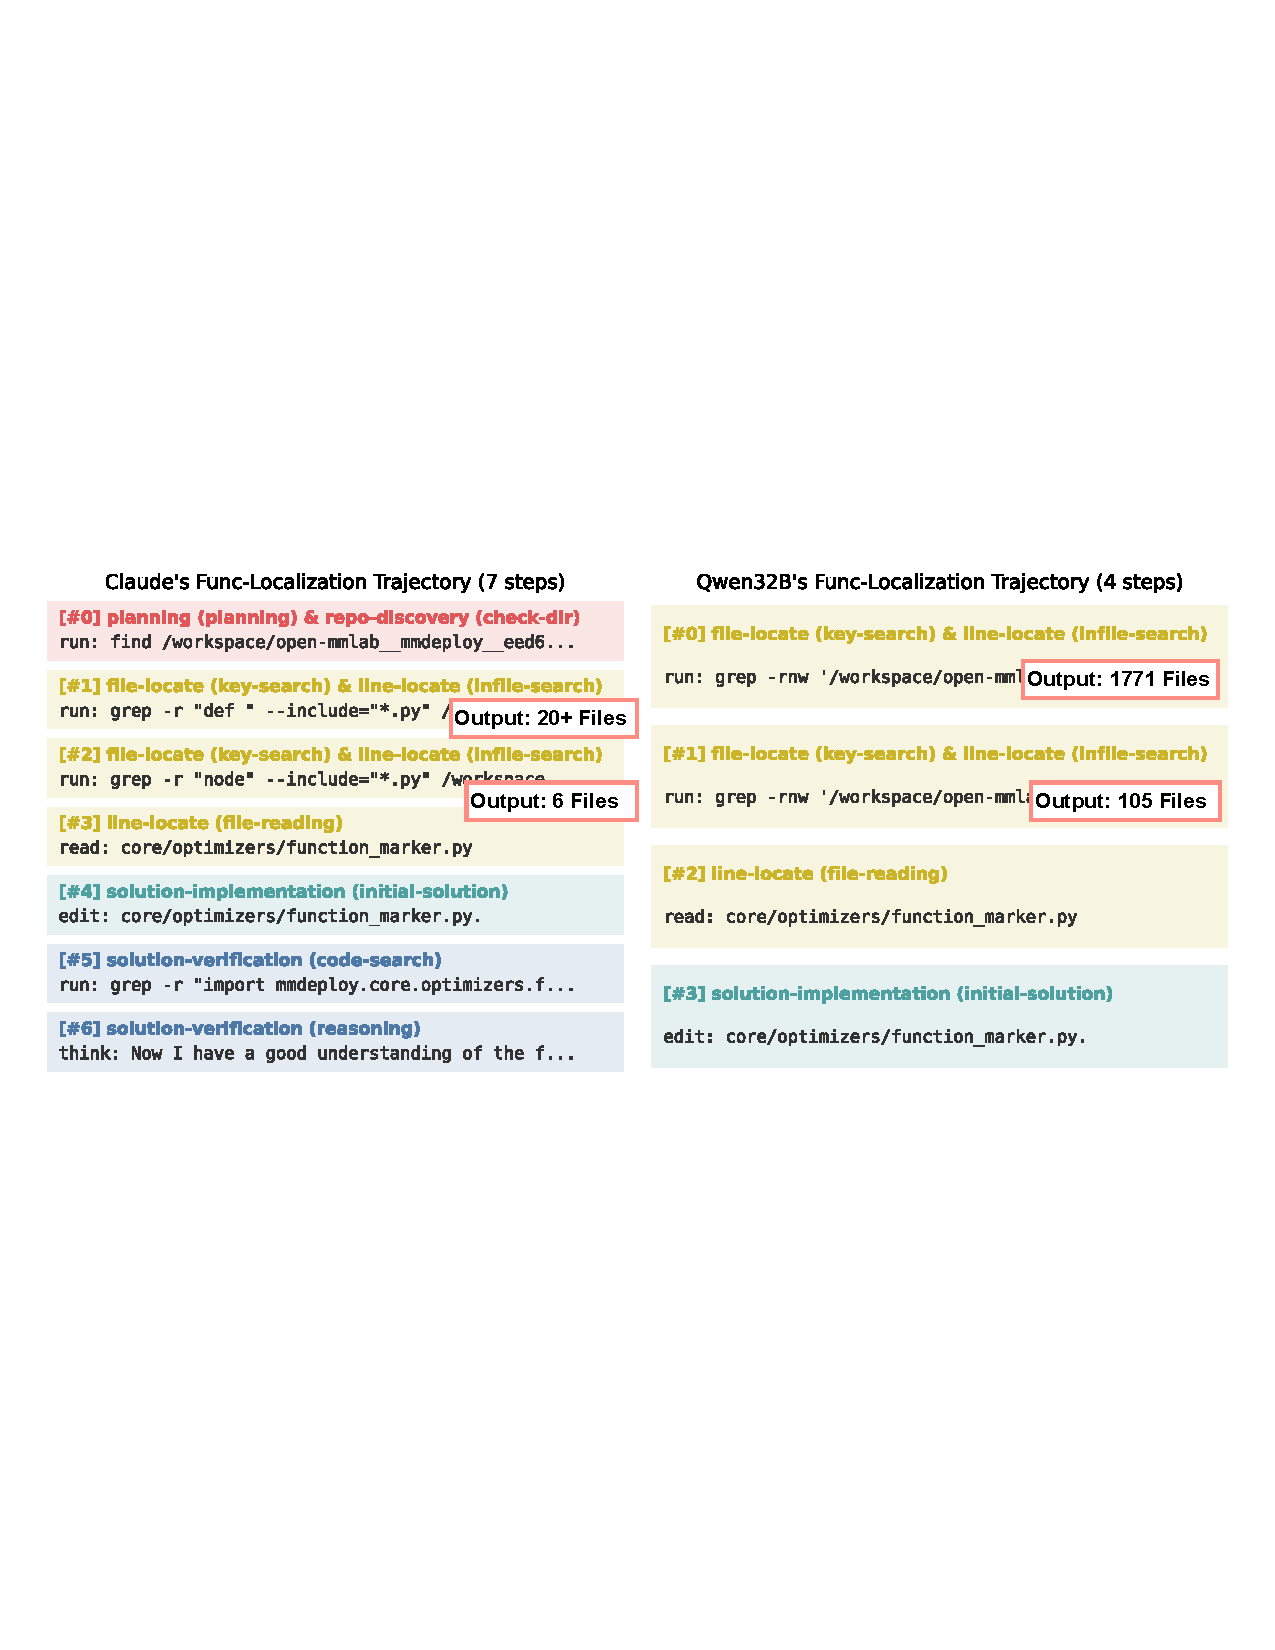
\includegraphics[width=\columnwidth]{plus_figs/trajectory_comparison.pdf}
  \caption{An example of how we represent trajectories at different abstraction levels. We show the categorization of each agent step in the format of ``stage label (strategy label)''. Note that the agent step can be categorized into multiple stages and strategies.}
  \label{fig:plus:abstraction}
\end{figure}


\section{Proposed Method 1: Candidate Agent Behavior Discovery for Different Abstraction Levels}
\label{plus:sec:categorization}
\subsection{Proposed Method}
Previous work and our preliminary experiments discover candidate agent behaviors by presenting the entire successful trajectories generated by two teacher models as context to an LLM agent and prompting it to discover different behaviors, which is still challenging for the agent.
Towards this challenge, our key intuition is that agent behaviors arise at different abstraction levels, and discovering them does not always require access to the full trajectory.
For example, we only need the high-level summary of the trajectory to identify whether an agent repeatedly performs verification after implementation.
Another example is that to compare the strategy used by the agent to localize a function, we only need to look at the function localization steps rather than the entire trajectory.

In summary, we categorize agent behaviors into three abstraction levels: \textbf{stage-level}, \textbf{stage-strategy-level}, and \textbf{step-level}, which enables us to design different types of context for the LLM agent to discover the behaviors at different levels.


\start{Represent Trajectories at Different Abstraction Levels}
The categorization of agent behaviors is based on how we represent each agent step at different abstraction levels.
In particular, we define:
\begin{itemize}
  \item \textbf{The Stage of Coding Tasks}: Build upon the analysis of Hybrid-Gym~\cite{hybrid-gym}, we pre-define the stages that are shared across different coding tasks: planning, repository discovery (e.g., checking the structure of the repository), file localization, code-line localization, code reproduction, solution implementation, and solution verification. Based on the analysis in Hybrid-Gym, the stages are shared across three downstream coding tasks: issue-solving, test generation, and library construction, and four synthetic training tasks: function localization, issue localization, dependency search, and function generation.
  \item \textbf{The Strategy to Complete a Stage}: For each stage, we define the strategy to complete the stage, or equivalently, the purpose of each action that is used to complete the stage. For instance, for the code-line localization stage, the strategy includes searching for keywords inside candidate files, reading the candidate files, executing relevant code and observing the error message, etc.
\end{itemize}

As shown in \autoref{fig:plus:abstraction}, given a set of trajectories, we assign a stage label and a strategy label to each agent step. 
We iteratively update the categories when we conducting new analyses and discovering new agent behaviors.
We keep adding new stages or strategies if we find agent steps that are not covered by the existing categories.
We can also break down a category into smaller categories if we find that it is too broad.



\start{Agent Behaviors at Different Abstraction Levels}
We categorize the agent behaviors based on which abstraction level of trajectory they are be represented at.
\begin{itemize}
  \item \textbf{Stage-level Behaviors}: the presence, order, or transition of different stages in the trajectory.
  For example, as shown in \autoref{fig:plus:abstraction}, Claude-3.7 has a ``solution verification'' stage after ``solution implementation''.
  % transits from the ``file localization'' stage to the ``function localization'' stage only when the number of candidate files is reduced to a limited number.
  \item \textbf{Stage-strategy-level Behaviors}: the presence, order, or transition of different strategies to complete a particular stage.
  For example, as shown in \autoref{fig:plus:abstraction}, for the function localization stage, Claude-3.7 performs several keyword searching actions that present both the file and the located lines of code. Then it perform file-reading actions to read the corresponding lines.
  \item \textbf{Step-level Behaviors}: properties of the specific messages generated by the agent. For instance, the agent correctly uses the ``file-editing'' tool to generate code patches with no errors and retries. Another example is that the agent generates long reasoning before generating the actions.
\end{itemize}

Note that in Hybrid-Gym~\cite{hybrid-gym} (\autoref{chap:hybrid-gym}), we present three principles for effective task design: (1) the tasks should generate a code patch as the outcome, (2) the tasks should involve a meaningful repository-exploration phase, and (3) the tasks should require non-trivial reasoning.
All the three principles can be translated to the agent behaviors with our definition: (1) the trajectory contains the ``solution implementation'' stage, (2) the trajectory contains the ``repository discovery'', ``file localization'', or ``code-line localization'' stages, and (3) the trajectory contains the ``planning'' stage, which are all stage-level behaviors. In this study, we conduct a more comprehensive analysis by including behaviors from all the three levels.


\start{Discovering Candidate Agent Behaviors at Different Abstraction Levels}
Similar to the preliminary experiments, we use an LLM agent to discover different agent behaviors in the two sets of trajectories.
In addition to access to the entire trajectories, we provide different context for the discovery of behaviors at different levels.
For stage-level behaviors, we provide the trajectories that are abstracted with the stage labels.
For stage-strategy-level behaviors, we provide the steps in the trajectories that belong to a particular stage. We additionally provide the strategy labels of these steps.
For step-level behaviors, we do not provide additional context other than the full trajectories, but we explicitly prompt the LLM agent to focus on the content of the single step.

The agent iteratively discovers new candidate behaviors based on the differences between the frontier and weaker teacher model's successful trajectories, examines whether the behaviors are well-defined and distinguishing, and discovers new candidate behaviors.


\subsection{Proposed Experiments}
We follow the preliminary experiments and compare the trajectories generated by a frontier and a weaker teacher model (e.g., Claude-3.7 and Qwen2.5Coder-32B). We start with training on the function localization task and evaluating on the SWE-Bench Verified issue-solving dataset. We will then extend the analysis to multiple teacher model pairs and multiple coding agent training tasks, which will be introduced in \autoref{plus:sec:extend-exp}.

Since the goal is to discover the agent behaviors that lead to the different distillation performances, we examine the two properties of each candidate agent behavior we discover: (1) Well-defined. (2) Distinguishing.

\start{Verification of Well-defined Agent Behaviors}
An agent behavior is well-defined if there exists a deterministic method to determine whether a trajectory contains the behavior. Furthermore, the behavior can be represented by a binary feature. For instance, the agent behavior ``using keyword searching to locate functions inside files'' is well-defined, but the agent behavior ``has comprehensive repository exploration'' is not, because it is ambiguous and does not have a precise operational definition.

For each candidate behavior, we use an LLM-based annotator to determine whether the behavior is present in a trajectory. The annotator outputs one of three labels: \texttt{present}, \texttt{absent}, or \texttt{unable\_to\_determine}. The annotation prompt includes the behavior definition and the formatted trajectory. To reduce annotation noise, we use a fixed prompt template and keep the annotator model unchanged across all experiments. 
We additionally validate the LLM annotations based on its agreement with human annotations on a small subset of trajectories.

To verify whether a candidate agent behavior is well-defined, we randomly sample $k$ instances where both of the two teacher models generate a successful trajectory, and apply the LLM-based annotator to all of the $2k$ trajectories. We compute the rate of \texttt{unable\_to\_determine} outputs for that behavior. We only retain behaviors whose indeterminate rate is below a threshold $\tau$ (e.g., $5\%$).


\start{Verification of Distinguishing Agent Behaviors}
To verify whether an agent behavior is distinguishing, similar to the above experiment, we randomly sample $k$ successful trajectories from each of the two teacher models and apply the LLM-based annotator to all of the $2k$ trajectories.

For each well-defined behavior, we define a binary feature for each trajectory: 1 the behavior is present in trajectory, and 0 otherwise.
We then test whether the prevalence of this behavior differs significantly between the two teacher models. Since this feature is binary, we use a chi-square test as the statistical test. 

Specifically, we construct a $2 \times 2$ contingency table over \{teacher model A, teacher model B\} and \{behavior present, behavior absent\}, and compute a p-value for the null hypothesis that the behavior occurs at the same rate in both models. We retain behaviors with a p-value below a threshold $\delta$ (e.g., $0.05$).



\section{Proposed Method 2: Controlled Experiments based on Trajectory Editing}
\label{plus:sec:controlled-exp}
\subsection{Proposed Method}
The goal of this part is to verify whether particular agent behaviors affect distillation performance.
A main limitation of the preliminary experiments is that, even if we prompt the teacher model to exhibit or avoid a target behavior, the model may not reliably follow the instruction. 

To address this limitation, we propose to conduct controlled experiments by directly editing the training trajectories to add, remove, or modify a target behavior whenever such editing is feasible.

The key intuition behind trajectory editing is that we only focus on trajectories that \emph{successfully} solve the task.
If an agent successfully solves the task, it is also likely to produce the \emph{essential intermediate outcomes} when completing the task.
For example, in the function localization task, where the agent must identify a target function from its description and generate a docstring for it, it is likely that the agent sees the target filename and the function content in some of the action outputs, and there must exist a step that edits the target function.
This observation makes it possible to edit some behaviors locally while preserving the overall consistency of the problem-solving process, as long as the edited part is producing the same essential intermediate outcome.
In other words, trajectory editing is suitable for behaviors that do not alter the essential intermediate outcome, but only changes \emph{how} the agent reaches or expresses that outcome.



\start{Principles of Trajectory Editing}
The main challenge of trajectory editing is to ensure that the edited trajectory remains \emph{consistent}. Here, consistency means that the edited trajectory still constitutes a valid successful problem-solving process, where (1) at least one step must still produce the final task outcome (e.g., a code patch that satisfies the task requirements), and (2) each step must have sufficient information from the previous context to justify its action.

We define a set of rules describing when trajectory steps can be added, removed, or modified without affecting the trajectory's consistency:
\begin{itemize}
    \item \textbf{Equivalent step substitution.} If two sets of agent steps require the same context and produce the same essential intermediate outcome, then one can be substituted for the other without affecting trajectory consistency. For example, in the file localization stage, the agent may perform search with different keywords. As long as target file appears in the search results, we can substitute the search steps.
    
    \item \textbf{Removal of non-essential steps.} Steps that do not provide necessary information for any subsequent step can be removed. Examples include file-search actions that do not lead to relevant results, verification of the generated code patch after it is already applied, or any actions that are failed to applied because the syntax is incorrect. 
    Note that removing such steps may make some later actions appear less well-motivated or less sound, but the trajectory still remains consistent.
    
    \item \textbf{Editing textual content.} The textual content of a step can be modified as long as the revised content remains consistent with the previous context. The reason is that only the action generated by the agent will be executed, and the execution output is not affected by the textual content.
    For instance, an action rationale may be rewritten to be more concise, or a message may be rephrased without changing the information it conveys.
\end{itemize}

We would like to note that these rules serve as an initial set of editing principles rather than a complete characterization. 
As the project progresses, we will introduce additional editing rules when new trajectory patterns and edge cases are identified.





\start{Examples of Controlled Experiment Design based on Trajectory Editing}
In \autoref{tab:plus:controlled-editing-examples}, we provide examples of how to design controlled experiments to verify the importance of a particular candidate agent behavior. Each example corresponds to a principle of trajectory editing we defined above.

% Candidate agent behavior: (stage-strategy-level) when locating specific lines of code, only perform file reading when the number of candidate files is reduced to a limited number.
% Controlled experiment design: given two trajectories, where one of them starts file reading when the number of candidate files is still large, as shown in \autoref{fig:plus:abstraction}, we replace its file localization steps with the ones in the other trajectory, and train a student model on the edited trajectory.

% Candidate agent behavior: (stage-level) the agent verifies the solution after implementation.
% Controlled experiment design: we remove all the solution verification steps, and train a student model on the edited trajectory.

% Candidate agent behavior: (step-level) the agent uses the file-editing tool correctly, with no errors and retries.
% Controlled experiment design: we remove all the failed file-editing actions and their execution outputs, and train a student model on the edited trajectory.



\begin{table}[t]
  \centering
  \small
  \begin{tabular}{p{0.3\textwidth} p{0.65\textwidth}}
  \toprule
  \textbf{Candidate Agent Behavior} & \textbf{Controlled Experiment Design} \\
  \midrule
  
  \textit{(Stage-strategy-level)} When localizing specific lines of code, the agent only begins file reading after the number of candidate files has been reduced to a limited set. 
  &
  Given two successful trajectories, if one trajectory starts file reading while the candidate file set is still large, we replace its file-localization steps with the corresponding steps from another trajectory that first narrows down the candidate files before reading them. We then train a student model on the edited trajectory set and compare its distillation performance with that of a model trained on the original trajectories.
  \\[0.8em]
  
  \textit{(Stage-level)} The agent performs solution verification after implementation.
  &
  We remove all solution-verification steps from otherwise successful trajectories, while keeping the implementation steps and final successful outcome unchanged. We then train a student model on the edited trajectory set and compare its distillation performance against that of a model trained on the original trajectories.
  \\[0.8em]

  \textit{(Step-level)} The agent generates long reasoning before generating the actions (more than 30 tokens).
  &
  We prompt an LLM to elaborate the textual part in the agent steps so that the reasoning remains the same but the length is longer than 30 tokens. We then train a student model on the edited trajectory set and compare its distillation performance.
  \\
  
  % \textit{(Step-level)} The agent uses the file-editing tool correctly, with no errors or retries.
  % &
  % We remove failed file-editing actions and their corresponding execution outputs from successful trajectories, while preserving the final successful edit and all required preceding context. We then train a student model on the edited trajectory set and compare its distillation performance against that of a model trained on the original trajectories.
  % \\
  
  \bottomrule
  \end{tabular}
  \caption{Examples of candidate agent behaviors and the corresponding controlled experiment designs based on trajectory editing.}
  \label{tab:plus:controlled-editing-examples}
  \end{table}



\start{The Fallback Method: Prompt Engineering and Data Filtering}
Note that not all behaviors can be easily added or removed from the trajectory.
In such cases, we fallback to the prompt engineering and data filtering method, as introduced in the preliminary experiments.
Specifically, we rewrite the trajectory-generation prompt to encourage or discourage the target behavior, and then generate new trajectories under the modified prompt. Finally, we conduct data filtering and only keep trajectories that have or do not have the target behavior.


In case we found a large number of candidate behaviors that could potentially affect distillation performance, we prioritize the candidate behaviors that are directly related to the key outcome of the task (e.g., the final code patch and the function and file it locates for the issue-solving task).
We iteratively perform the discovery and verification processes until we cannot find any new candidate agent behaviors.



\subsection{Proposed Experiments}
For each candidate behavior, we construct two training sets with the same number of trajectories: a \emph{control} set that preserves the original trajectories, and an \emph{edited} set in which the candidate behavior is added or removed.
We train a student model on each of the two training sets, with all hyper-parameters fixed.
We then compare the two student models on downstream coding tasks (e.g., the SWE-Bench Verified issue-solving task) to determine whether editing the behavior leads to a measurable change in performance.

To reduce variance, we repeat each training comparison with multiple seeds (e.g., three seeds) and report the mean and variance of the distillation performance. We then test whether the edited and original conditions differ significantly using a two-tailed t-test.

We only keep the agent behaviors where the distillation performance on the two training sets are significantly different.



\section{Proposed Method 3: Extend to Multiple Models and Tasks}
\label{plus:sec:extend-exp}
\subsection{Proposed Method}
As an extension of the preliminary experiments, we propose to apply the analyses in \autoref{plus:sec:categorization} and \autoref{plus:sec:controlled-exp} to multiple teacher-model pairs and multiple coding-agent training tasks. The goal is to obtain a more comprehensive list of desired agent behaviors that affect distillation performance, and to verify whether the behaviors are transferable across different tasks.

The final outcome of this project will include:
\begin{itemize}
  \item a set of desired agent behaviors that have a positive effect on distillation performance;
  \item for each training task, a checklist over teacher models showing the proportion of successful trajectories that contain each desired behavior;
  \item a checklist over training tasks showing the proportion of successful trajectories that contain each desired behavior. Here we only consider the trajectories generated by the strongest teacher model.
\end{itemize}

Through this analysis, we expect to find that (1) teacher models with weak distillation performance are missing one or more of the desired behaviors identified in our controlled experiments, and (2) at least a subset of these desired behaviors are shared across different coding-agent training tasks. 


\subsection{Proposed Experiments}
We propose to repeat the analyses in \autoref{plus:sec:categorization} and \autoref{plus:sec:controlled-exp} by comparing Claude-3.7 with several weaker teacher models from different model families: GPT-5-mini~\cite{gpt5}, Gemini-3.1-Flash-Lite~\cite{gemini3flash}, and Qwen2.5-Coder-32B~\cite{qwen25coder}. 
We choose these models in part based on serving cost, with the goal of focusing on teacher models that are substantially cheaper than Claude-3.7, yet still capable of producing successful trajectories for meaningful comparison.

We further propose to conduct these comparisons across a diverse set of training tasks, including SWE-Gym issue solving~\cite{swegym}, Hybrid-Gym function localization and function generation~\cite{hybrid-gym}. 
All the tasks are shown to be effective for generalizing to the issue-solving task.
This enables us to verify whether the desired behaviors are transferable across different tasks.




\part{Training Critique Models to Assist Coding Agents}
\label{part:usage}


\start{Overview of Part~\ref{part:usage}}
In \autoref{part:scalability} and \autoref{part:generalizability}, we aim to construct synthetic data to improve coding agent effectiveness. However, such methods are inherently bottlenecked by the capacity of the base models.
To address this limitation, in this part, we develop an auxiliary model to assist the primary coding agent. With the auxiliary model in the context, the search space of the coding agent's actions is reduced. Therefore the system can achieve potentially better performance with the same capacity of the coding agent.

Specifically, we identify two key principles that an ideal auxiliary model should follow: (1) it should provide additional performance gains when collaborating with the primary coding agent, and (2) it should specialize in capabilities that are different from the main coding agent.
We then show that a critique model that is trained to provide textual critiques for the main model during inference can achieve both principles, for both seq-to-seq NLP tasks (\autoref{chap:fence}) and coding agent tasks (\autoref{chap:prm-training}).

In \autoref{chap:fence}, we show that a critique model can improve the factuality of a generator model by either interacting with it in inference or providing feedback to assist training. We further improve the effectiveness of the critique model by constructing tailored training data.

When it comes to the domain of coding agent, in a \proposedWork (\autoref{chap:prm-training}), we first show that using a frontier model (e.g., Claude) to provide critique during inference substantially improves the correctness of a coding agent. Then we distill a more cost-efficient critique model by constructing synthetic supervised-finetuning training data. To further improve its effectiveness, we propose a method to construct direct preference optimization (DPO) training data, focusing on its gap between the frontier critique model.



\chapter{Improving Generator Factuality by Training an Evaluator Model}
\label{chap:fence}

\begin{figure}[t]
\centering
    \centering
    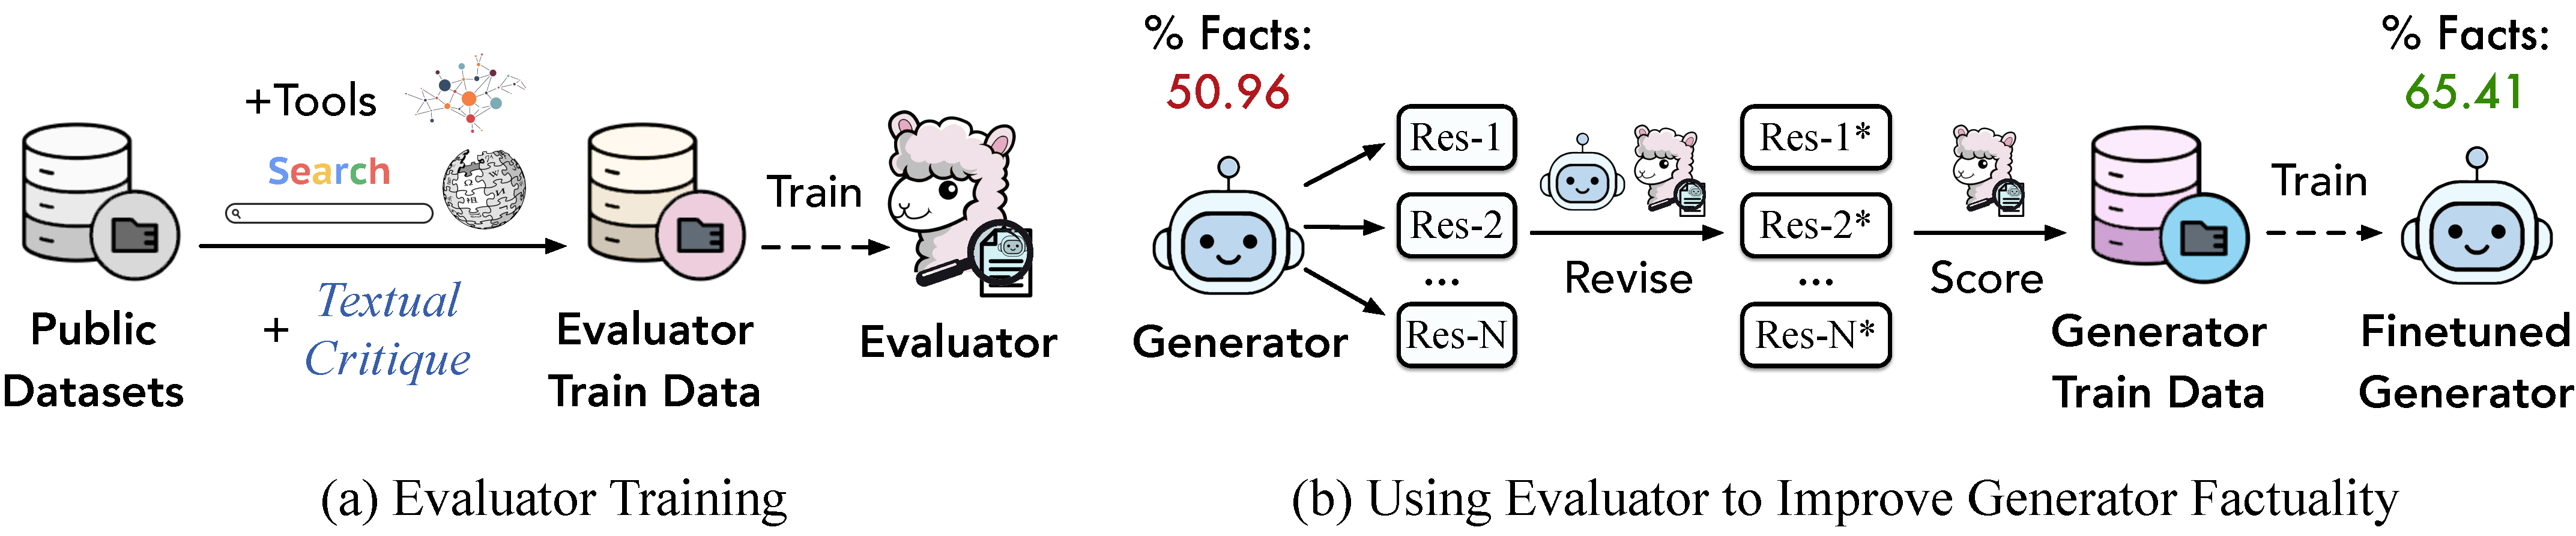
\includegraphics[width=\linewidth]{FenCE_figures/overall.pdf}
    \upv
    \caption{\textit{(Left)} The framework to train an evaluator, \fencemodelname, by augmenting public datasets with textual critiques and more diverse knowledge sources. We show the details in \autoref{fig:evaluator_train}.
    \textit{(Right)} The framework to improve model factuality with \fencemodelname. We construct training data by leveraging \fencemodelname to revise and score the generator's responses. Details of response revision are shown in \autoref{fig:revise}.}
    \label{fig:overview}
    \downv
\end{figure}

\section{Introduction}
Hallucination is one of the persistent challenges for large language models (LLMs), where models generate plausible-sounding but incorrect information, even if they are shown factual information during pretraining~\citep{hallucination-survey,empirical-factuality}. 
One hypothesis is that LLMs fail to distinguish the boundary between memorized facts and other plausible-sounding information and do not learn to only output memorized facts, especially on their unfamiliar topics~\citep{finetuning-on-new,understand-finetuning,unfamiliar-finetuning}.
Although it is possible to reduce hallucination in inference with decoding strategies~\citep{ITI,DoLA} or post-editing~\citep{FAVA,EVER}, they introduce severe latency issues and hurts efficiency in real-time applications.


Alternatively, prior studies train the generator to output more factual responses, by preferring (1)  generation candidates with higher factuality scores \citep{FactTune}, which is limited by the generator's capabilities, or (2) responses with false information corrected~\citep{EVER}, 
which is prone to introducing lesser-known facts.
As shown in recent work~\citep{finetuning-on-new,understand-finetuning}, such preference training reinforces the model to generate information not well memorized during pretraining, and hence could even hurt factuality.
Furthermore, the methods either leverage proprietary models that have restricted terms of use, or prompt the generator to evaluate its own factuality, which suffers from self-bias and leads to inaccurate judgments~\citep{self-bias}.


Recent work trains evaluator models that could potentially be used to provide training signals for generators.
One category of work relies on proprietary models (e.g., GPT-4) to generate training data in various formats~\citep{prometheus,AutoJ}.
In contrast, \citet{FLAMe} leverage public datasets containing judgments of whether a claim is factual against certain source documents. 
However, such documents are generally sampled from very \textbf{restricted sources} such as news corpora or Wikipedia, while an evaluator could potentially benefit from knowledge obtained by a multiplicity of tools (e.g., search engines)~\citep{longform}.
Furthermore, the judgment label in most datasets is a single binary or numeric score, providing \textbf{limited feedback} to the generator model.

In this paper, we present \fencemodelname, a \textbf{F}in\textbf{e}-grai\textbf{n}ed \textbf{C}ritic-based \textbf{E}valuator that aims to provide textual critiques for each model-generated claim based on diverse knowledge sources.
We start with a set of public datasets with human judgments on the factuality of model-generated claims. 
As shown in \autoref{fig:overview}(a), we augment the judgment labels with textual critiques, which provide more informative and explainable feedback to the generator.
In addition, we augment the source documents by invoking multiple tools, including a search engine, knowledge base, and knowledge graph, with the goal of training the evaluator to leverage more diverse knowledge sources.

We further demonstrate how to leverage \fencemodelname to improve the generator's factuality with finetuning.
To construct training data (\autoref{fig:overview}(b)), we generate multiple responses for each prompt, use \fencemodelname to judge and critique every claim in the responses, and replace false information with facts or remove it from the response, depending on whether the corresponding fact is within the generator's knowledge 
(i.e., whether the generator outputs \textit{``unknown''} when prompted about claim correctness). 
This mitigates introducing lesser-known facts into training data.
% \dpfried{this is interesting! People might wonder how it's done. Is it possible to convey this using just a few words?}
Finally, unlike existing work that use the generator itself as the evaluator, we use \fencemodelname to score each original and revised response and construct preference data, which reduces self-bias and produces more accurate judgments.


Experiments show that \fencemodelname outperforms large open-source models such as Mistral-123B and strong proprietary models such as Claude-3 on LLM-Aggrefact.
With \fencemodelname, we improve Llama2-7B-chat's factuality by 16.86\% on FActScore~\citep{factscore} and 17.64\% on TruthfulQA \cite{truthfulqa}, outperforming existing factuality finetuning methods by 8.83\% and 3.99\%, respectively.
Analyses further show that after training with our recipe, the generator outputs less information for unfamiliar entities and more information for popular ones, suggesting that it learns to only generate information that is likely to be factual.

\start{Contributions}
(1) We train a fine-grained critique-based evaluator, \fencemodelname, by augmenting public datasets with textual critiques and more diverse source documents.
(2) We propose a training recipe to improve the generator's factuality by leveraging \fencemodelname to improve and score its responses.
(3) We conduct extensive experiments to validate both the judgment accuracy of \fencemodelname and the factuality of the generator trained with \fencemodelname, outperforming state-of-the-art factuality training methods by 8.83\% on FActScore and 3.99\% on TruthfulQA.





\section{Methodology}

\begin{figure}[t]
\centering
    \centering
    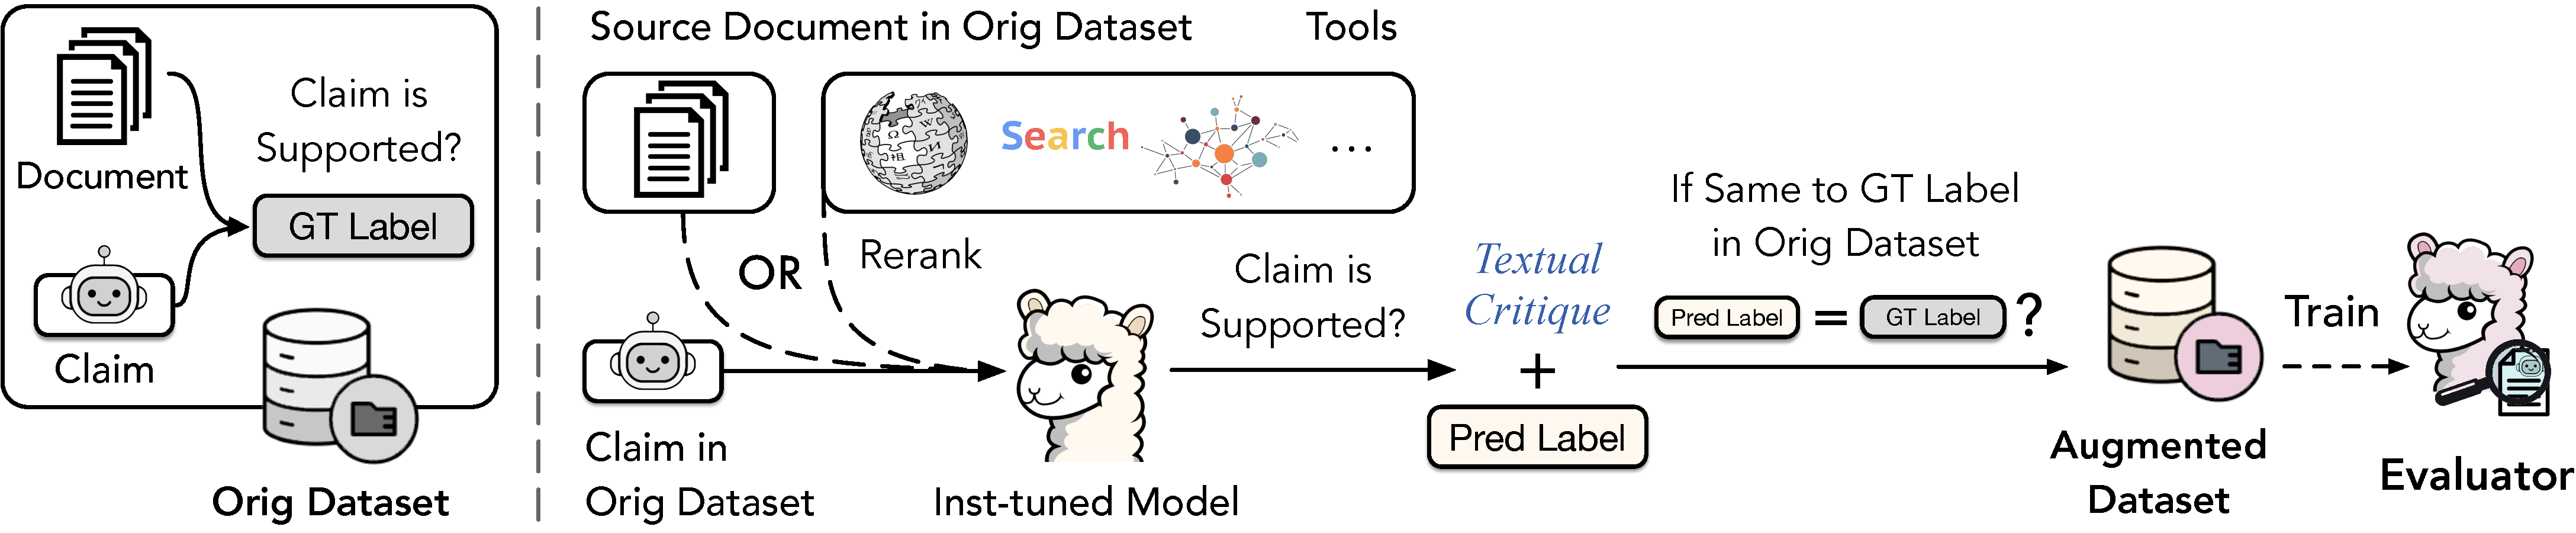
\includegraphics[width=\linewidth]{FenCE_figures/evaluator_train.pdf}
    \upv
    \caption{Framework of evaluator training. (\textit{left}) Existing public datasets for evaluator training. Each example contains a claim, a source document, and the ground truth (GT) label of whether the claim is supported by the document. (\textit{Right}) We augment the datasets with textual critiques and more diverse source documents obtained by tools. We use zero-shot Llama-3-70B-chat as the instruction-tuned model in our experiments.}
    \label{fig:evaluator_train}
    \downv
\end{figure}

\subsection{\fencemodelname: Factuality Evaluator Training}
\label{sec:evaluator_training}

\start{Preliminary}
To train the evaluator to recognize hallucinations, previous work~\citep{FLAMe} incorporates a combination of datasets with human judgments on factuality. As shown in \autoref{fig:evaluator_train}, in most datasets, each example contains a claim, a source document, and the ground-truth judgement of whether the claim is (1) fully supported by, (2) contradicted with, or (3) contains information that cannot be verified by the document.



We formally define the problem as follows:
Given a claim $c \in \mathcal{C}$, a source document $d \in \mathcal{D}$, a factuality evaluator aims to learn a mapping $f: \mathcal{C} \times \mathcal{D} \rightarrow \mathcal{L}$, which maps each claim-document pair $(c,d)$ to one of the labels:  
$f(c,d) = l \in \mathcal{L} =$ \{\textit{Supported, Contradictory, Unverified}\}.



\start{Augmenting Labels with Textual Critiques}
In addition to the classification label, we aim to train the evaluator to generate a \textit{textual critique} that explains the judgement, which provides more informative feedback such as which part of the document supports or contradicts the claim. We will leverage such feedback to revise generator responses and use them to train a more factual generator (see \S\ref{sec:improve_factuality} for details).
Formally, we aim to learn the mapping $f: \mathcal{C} \times \mathcal{D} \rightarrow \mathcal{R} \times \mathcal{L}$, which maps each claim-document pair $(c,d)$ to both the textual critique $r \in \mathcal{R}$ and the label $l \in \mathcal{L}$.


As shown in \autoref{fig:evaluator_train}, we prompt an instruction-tuned model $\mathcal{M}$ (e.g., Llama3-70B-chat) to generate both the critique $r_\mathcal{M}$ and label $l_\mathcal{M}$ for whether a claim $c$ is supported. The critique and label are likely to be consistent because the label is generated conditioned on the critique. As a result, if the predicted label $l_\mathcal{M}$ aligns with the ground truth label $l_{GT}$ in the original dataset, the critique is also likely to be aligned and we hence use both the critique $r_\mathcal{M}$ and label $l_\mathcal{M}$ as the new training target. Otherwise, if the predicted label does not align with the ground truth, we discard the whole example.



\start{Augmenting Source Documents using Tools}
To judge the factuality of an arbitrary model-generated claim, we could potentially benefit from \textit{a multiplicity of tools} such as search engines or online knowledge bases. However, the source documents in existing judgment datasets typically come from very restricted sources, such as news corpora or Wikipedia.
To bridge this gap, we obtain additional source documents for each claim by calling the following tools: a search engine (Bing Search API), knowledge base (Wikipedia), and knowledge graph (Google Knowledge Graph API).


As shown in \autoref{fig:evaluator_train}, given the claim $c$ in the original dataset, we prompt an instruction-tuned model to call multiple tools to verify the factuality of the claim (i.e., by generating tool calls such as search queries).
Then we rerank the returned results to obtain a combination of tool-extracted documents $d_t$. 
Similar to critique generation, we prompt the instruction-tuned model $\mathcal{M}$ to predict whether claim $c$ is supported by the tool-extracted documents $d_t$. We add $d_t$ to the train set if the predicted label $f_\mathcal{M}(c, d_t)$ is the same as the ground truth label $f_{GT}(c, d)$ in the original dataset.

The intuition is that if a claim can be supported by some documents, it is likely that we can obtain other supporting sources by calling the tools.
If a claim is hallucinated, it is very unlikely to find any knowledge that supports it with any tools. In both cases, we have $f_{GT}(c, d_t) = f_{GT}(c, d)$.



\start{Training Objective}
After obtaining the augmented training data $\mathcal{TR}_{Eval}=\{(c,d),(r,l)\}$, where each example contains (claim $c$, source document $d$, critique $r$, label $l$), we initialize the evaluator $\mathcal{E}$ with a instruction-tuned model and train it with a standard conditional language modeling objective, maximizing likelihood:
\begin{equation}
    \max _{\mathcal{E}} \mathbb{E}_{(c,d),(r,l) \sim \mathcal{TR}_{Eval}} \log \mathbb{P}_{\mathcal{E}}(r, l \mid c, d).
\label{eq:evaluator_sft}
\end{equation}


\begin{figure}[t]
\centering
    \centering
    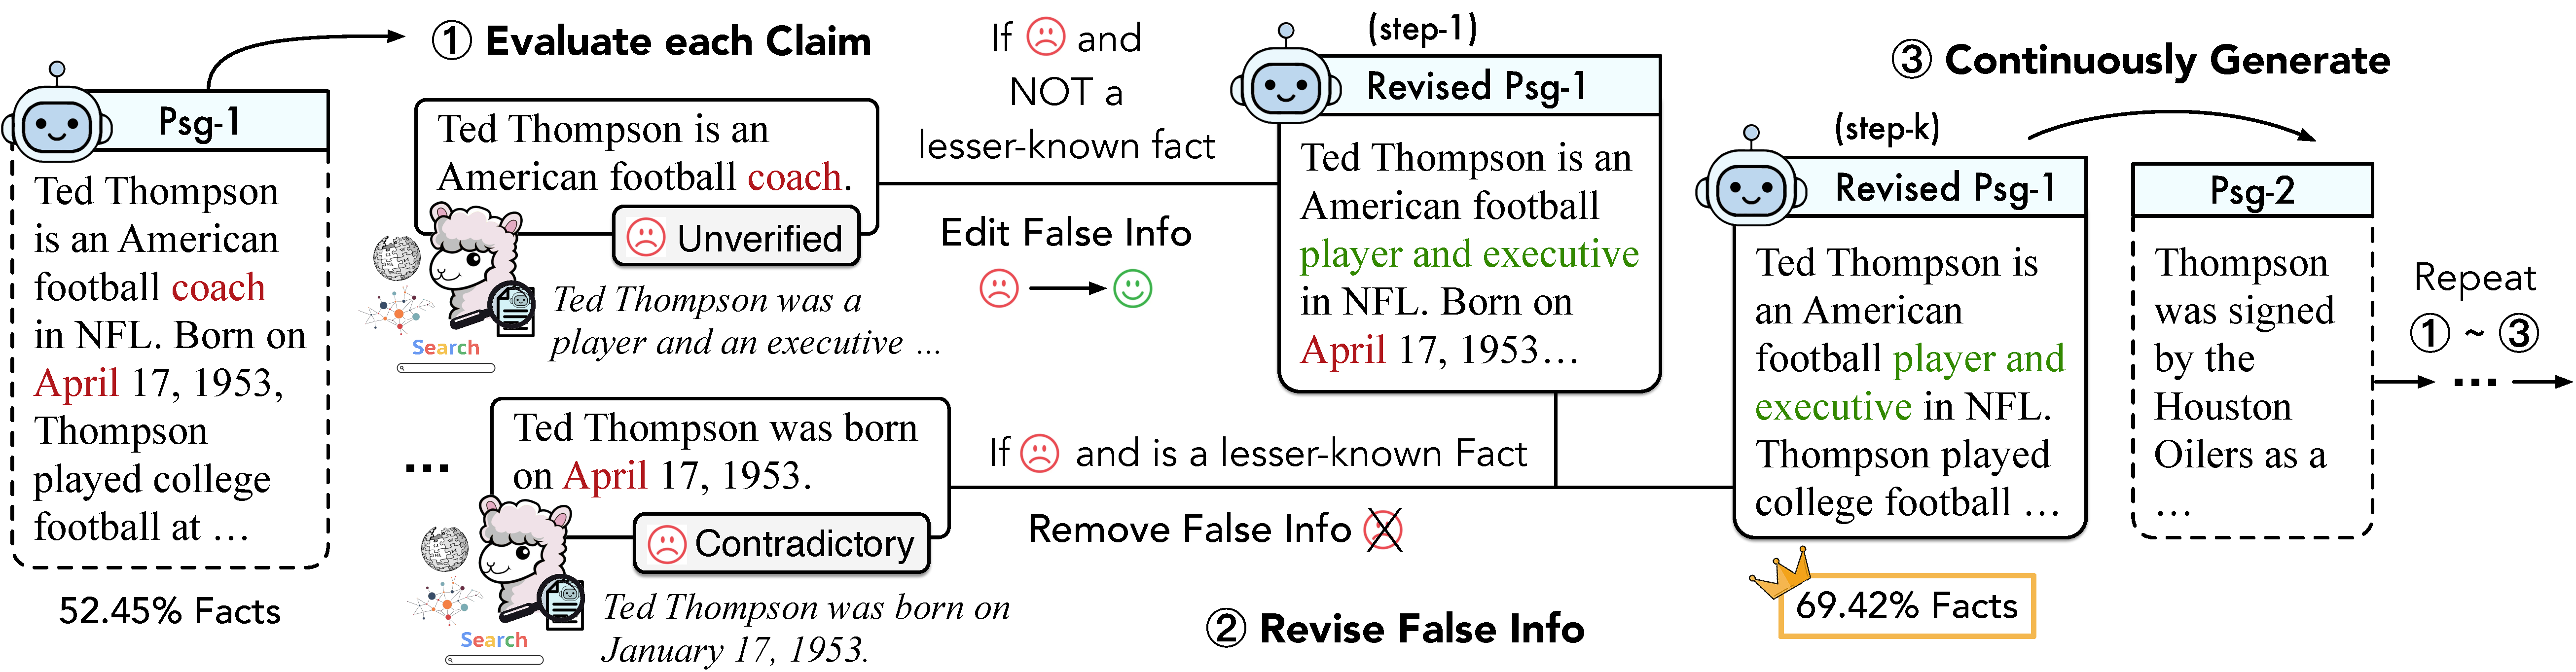
\includegraphics[width=\linewidth]{FenCE_figures/improve_factuality_v2.pdf}
    \upv
    \caption{
    The framework to revise model responses without introducing lesser-known facts. 
    We iteratively 
    (1) use \fencemodelname to evaluate the factuality of each claim, 
    (2) replace false information (if any) with the correct fact or remove it from the response, depending on whether it corresponds to a lesser-known fact,
    and (3) continue generating the next passage. 
    For every claim, we prompt the generator ``\textit{Is this claim factual?}'' without providing any source documents. If the generator outputs \textit{``unknown''}, we assume that the claim corresponds to a lesser-known fact.
    }
    \label{fig:revise}
    \downv
\end{figure}


\subsection{Improving Generator Factuality with \fencemodelname}
\label{sec:improve_factuality}
In this section, we use our evaluator, \fencemodelname, to improve a generator model's factuality, where we construct training data by revising and scoring the generator's own responses.
Compared to directly training the generator on factuality datasets, our method only requires a prompt set as inputs and hence enjoys much better scalability.

\start{Overview}
As shown in \autoref{fig:overview}, given a prompt, we use the generator to generate $N$ candidate responses.
Then we improve the factuality of each response by using \fencemodelname to evaluate the factuality of each piece of generated information and editing or removing the false information, depending on whether the corresponding fact is rare.
Finally, we use \fencemodelname again to score all original and revised responses and construct training data.

\start{Response Revision}
We aim to improve the factuality of the generator's responses \textit{without introducing lesser-known facts} to training data. The motivation is that as shown in recent research~\citep{understand-finetuning,finetuning-on-new}, forcing the model to generate lesser-known facts that are poorly memorized during pretraining will blur the boundary with memorized facts and other plausible sounding information, which may lead to even more hallucination.
As shown in \autoref{fig:revise}, we iteratively revise each passage with the following three steps: 

\quad [\underline{\textbf{Step}-\circled{1} \textbf{Evaluate}}] 
we prompt an instruction-tuned model (e.g., Llama3-70B-chat) to decompose each response into claims. Then for each claim, we call tools to obtain related documents and apply \fencemodelname to evaluate its factuality with critique. 

\quad [\underline{\textbf{Step}-\circled{2} \textbf{Revise}}] 
If there are any claims that are judged as \textit{``unverified''} or \textit{``contradictory,''} we further check whether it corresponds to a lesser-known fact. 
Specifically, we prompt the generator \textit{``Is this claim factual?''} and output \textit{``true,''} \textit{``false,''} or \textit{``unknown,''} without providing it any external knowledge. We regard the claim as a lesser-known fact if the generator outputs \textit{``unknown.''}

If the claim does not correspond to a lesser-known fact, we prompt the generator to correct the false information based on the critique generated by \fencemodelname. Otherwise, we prompt the generator to remove the false information from the passage.

\quad [\underline{\textbf{Step}-\circled{3} \textbf{Generate}}] 
To reduce error propagation, we use the revised passages as the prefix and continuously generate the next passage.


\start{Generator Training}
We use \fencemodelname to score each original and revised response by computing the percentage of factual claims. Then we train the generator with first supervised finetuning (SFT) and then direct preference optimization (DPO)~\citep{DPO}.
In the SFT stage, we train the generator with the top-$k$ responses as targets, where the responses are ranked by the percentage of factual claims, optimizing with the conditional language modeling objective, which is similar to \autoref{eq:evaluator_sft}.

In the DPO stage~\citep{DPO}, we construct preference data $\mathcal{TR}_{Gen}= \{x, y_w, y_l\}$ as follows: for each prompt $x$, we choose the preferred response $y_w$ from the top-$k$ responses and choose any responses with lower scores than $y_w$ as the rejected response $y_l$.
Suppose we have $N$ original and $N$ revised responses, this gives us $\binom{2N}{2} - \binom{2N-k}{2}$ preference pairs.
We initialize the generator from the SFT checkpoint and optimize the following classification loss:
\begin{equation}
\begin{aligned}
    \max _{\mathcal{G}} 
    \mathbb{E}_{\left(x, y_w, y_l\right) \sim \mathcal{TR}_{Gen}}
    & \left[\right.
    \log \sigma
    \left(\right. \beta 
    \log \frac{\pi_\mathcal{G}\left(y_w \mid x\right)}{\pi_{\text {ref}}\left(y_w \mid x\right)} \\
    & -\beta 
    \log \frac{\pi_\mathcal{G}\left(y_l \mid x\right)}{\pi_{\text {ref}}\left(y_l \mid x\right)}
    \left.\right)
    \left.\right],
\end{aligned}
\end{equation}

where $\sigma$ is the Sigmoid function. The reference policy $\pi_{\text {ref}}$ is computed by the SFT checkpoint.






\section{Experiments on Evaluator Training}
In this section, we aim to answer the research question: (\textbf{RQ1}) Can \fencemodelname correctly judge the factuality of model-generated claims?




\subsection{Experimental Setup}
\start{Training Details}
We initialize \fencemodelname from Llama3-8B-chat and train it on a set of public factuality judgment datasets, which \citet{FLAMe} is trained on.
To ensure label accuracy, we focus on datasets with human judgment on model responses, including summarization datasets: XSum Hallucination~\citep{xsum-hallucination}, QAGS~\citep{QAGS}, FRANK~\citep{FRANK}, question-answering datasets: RAGTruth~\citep{ragtruth}, FActScore~\citep{factscore}, and dialogue datasets: Q$^2$~\citep{Q2}, FaithDial~\citep{faithdial}, BEGIN~\citep{begin}.
% We provide implementation and dataset details in \S\ref{sec:implementation_details} and \S\ref{sec:data_details}.


\start{Evaluation Dataset and Metric}
We evaluate the evaluators on the LLM-AggreFact benchmark~\citep{llm-aggrefact}, a combination of 10 datasets covering three tasks: fact verification, summarization, and long-form QA.
All datasets contain human-annotated (document, claim, label) tuples. 

We follow \citet{llm-aggrefact} and use balanced accuracy (BAcc) as the evaluation metric: $\text{BAcc} = \frac{1}{2}\left(\frac{\mathrm{TP}}{\mathrm{TP}+\mathrm{FN}}+\frac{\mathrm{TN}}{\mathrm{TN}+\mathrm{FP}}\right)$, where $\mathrm{TP}$, $\mathrm{TN}$, $\mathrm{FP}$, and $\mathrm{FN}$ represent true/false positives/negatives. 


\start{Baselines and Ablations}
We compare to the LLM-based fact-checkers reported by \citet{llm-aggrefact}.
We do not include results reported in \citet{FLAMe} because they use a different metric.

In addition, we compare to two ablations: (1) \fencemodelname (\textit{Vanilla SFT}), which is trained on the original public datasets with no augmentation, and (2) \fencemodelname (\textit{Critique Only}), where we only generate textual critiques and not source documents.

\begin{table}[t]
\centering
\upv
\resizebox{\textwidth}{!}{
\begin{tabular}{lccccccccccc}
\toprule
& \multicolumn{10}{c}{\textbf{LLM-AggreFact} (\emph{without} threshold tuning)} & \\
\cmidrule(r){2-11} 

\multirow{2}{*}{\bf \quad Model Name} &
  \multicolumn{2}{c}{\textbf{\textsc{AggreFact}}} &
  \multicolumn{2}{c}{\textbf{\textsc{TofuEval}}} &
  \multirow{2}{*}{\textbf{\textsc{Wice}}} &
  \multirow{2}{*}{\textbf{\textsc{Reveal}}} &
  \multirow{2}{*}{\begin{tabular}[c]{@{}c@{}}\textbf{\textsc{Claim}}\\ \textbf{\textsc{Verify}}\end{tabular}} &
  \multirow{2}{*}{\begin{tabular}[c]{@{}c@{}}\textbf{\textsc{Fact}}\\ \textbf{\textsc{Check}}\end{tabular}} &
  \multirow{2}{*}{\begin{tabular}[c]{@{}c@{}}\textbf{\textsc{Expert}}\\ \textbf{\textsc{QA}}\end{tabular}} &
  \multirow{2}{*}{ \textbf{\textsc{Lfqa}}} &
  \multirow{2}{*}{\textbf{Avg}} \\
\cmidrule(r){2-3} \cmidrule(r){4-5} 
& \textbf{CNN}  & \textbf{XSum} & \textbf{MediaS} & \textbf{MeetB} & & & & & & & \\
\midrule
\dlrow \multicolumn{10}{l}{\textit{Open-source Models (Llama3-8B based)}} & & \multicolumn{1}{|c}{} \\
\quad Llama3-8B-chat & 50.9 & 58.2 & 63.9 & 72.4 & 65.1 & 85.2 & 63.8 & 76.5 & 55.9 & 72.3 & \multicolumn{1}{|c}{66.4} \\
\quad \fencemodelname \textit{(Vanilla SFT)} & \underline{63.2} & 73.4 & 66.6 & 77.7 & 64.6 & 86.4 & 72.5 & 73.0 & 57.9 & 83.1 & \multicolumn{1}{|c}{71.8} \\
\quad \fencemodelname \textit{(Critique Only)} & 59.5 & \underline{74.7} & 68.4 & 80.0 & 71.7 & 88.0 & \underline{74.3} & 74.2 & 59.6 & \textbf{87.0} & \multicolumn{1}{|c}{\underline{73.7}} \\
\quad \fencemodelname \textit{(Full)} & 62.1 & 72.4 & \textbf{70.9} & \textbf{80.3} & \underline{76.0} & \textbf{88.6} & \textbf{74.9} & 74.4 & \textbf{60.3} & \underline{86.9} & \textbf{74.7} \\
\midrule 
\dlrow \multicolumn{10}{l}{\textit{Other Open-source Models (47B-123B)}} & & \multicolumn{1}{|c}{} \\
\quad Mistral-8x7B$\dagger$ & 55.0 & 65.5 & \underline{68.5} & 73.3 & 63.8 & 80.8 & 64.3 & 75.1 & 56.3 & 70.8 & \multicolumn{1}{|c}{67.3}  \\
\quad Llama3-70B-chat & \bf 63.3 & 71.3 & 67.9 & 75.2 & 74.8 & 86.7 & 67.3 & \underline{78.3} & 58.4 & 82.9 & \multicolumn{1}{|c}{72.6} \\
\quad Mistral-123B$\dagger$ & 58.4 & \textbf{76.3} & 67.3 & \underline{78.9} & \bf 76.6 & \underline{88.4} & 67.6 & \bf 79.0 & \underline{60.0} & 81.7 & 73.4 \\
\midrule
\midrule 
\dlrow \multicolumn{10}{l}{\textit{Proprietary Models or Distilled Models}} & & \\
\quad Gemini-Pro$\dagger$ & 49.4 & 60.6 & 63.8 & 65.8 & 65.8 & 85.5 & 61.8 & 76.8 & 56.8 & 75.9 & \multicolumn{1}{|c}{66.2} \\
\quad GPT-3.5$\dagger$ & 63.2 & 72.4 & 66.8 & 73.4 & 68.5 & 84.7 & 65.2 & 70.8 & 57.2 & 73.8 & \multicolumn{1}{|c}{69.6} \\
\quad Claude-2.1$\dagger$ & 59.9 & 66.4 & 69.2 & 72.3 & 64.3 & 88.2 & 69.7 & 79.3 & 59.8 & 78.2 & \multicolumn{1}{|c}{70.7} \\
\quad Claude-3 Opus$\dagger$ & 65.2 & 72.4 & 74.1 & 82.4 & 75.0 & 83.8 & 69.3 & 78.8 & 58.8 & 81.6 & \multicolumn{1}{|c}{74.1} \\
\quad MiniCheck-FT5$\dagger$ & 69.9	& 74.3 & 73.6 & 77.3 & 72.2 & 86.2 & 74.6 & 74.7 & 59.0 & 85.2 & \multicolumn{1}{|c}{74.7} \\
\quad GPT-4$\dagger$ & 66.7 & 76.5 & 71.4 & 79.9 & 80.4 & 87.8 & 67.6 & 79.9 & 59.2 & 83.1 & \multicolumn{1}{|c}{75.3} \\

\bottomrule
\end{tabular}
}
\caption{Performance (BAcc) of evaluator models on the test split of LLM-AggreFact. We separate Llama3-8B-chat based models, larger open-source models, and proprietary models into different blocks. We highlight the best-performing open-source model for each dataset.
Results with $\dagger$ are reported in \citet{llm-aggrefact}.
} 
\label{tab:res-llm-aggrefact}
\end{table}


\subsection{Main Results}
As shown in \autoref{tab:res-llm-aggrefact}, after training on our augmented datasets, \fencemodelname improves Llama3-8B-chat by 8.3\% BAcc and outperforms all the open-source LLMs, including models with significantly more parameters (e.g., Mistral-123B). It also outperforms strong proprietary models such as Claude-3 Opus.
When compared with its ablations, \fencemodelname consistently outperforms the Vanilla SFT model on 8 out of 10 datasets, with average gain of 2.9\% BAcc.
The performance of \fencemodelname (\textit{Critique Only}) is between Vanilla SFT and the full model, which indicates the utility of both augmentation methods.

Among all the datasets, we observe that the performance on Wice decreases after Vanilla SFT, but is largely improved by \fencemodelname. 
One possible reason is that some training datasets such as Q$^2$ contain claims that are labeled as ``factual'' but are only partially supported by the documents.
We hypothesize that such noisy examples strongly affect the performance on Wice, which contains as high as 54.7\% of such ``partially supported'' examples.
However, by filtering out examples where Llama3-70B-chat cannot generate explanations, we filter out a large percent of such noisy examples and hence improve the final judgment accuracy.



\subsection{Result Analyses}
\start{Accuracy of Augmented Critique and Source Documents}
With our data augmentation methods, we equipped 77.2\% of the training examples with textual critiques, and generate new source documents for 54.1\% of the examples with the combination of our three tools. 
To verify the data quality, we randomly sampled 45 examples where we successfully obtain critiques or source documents (15 for each label) and manually inspect the accuracy.
Specifically, we check whether both the critique and the label correctly reflect the relationship between the claim and the source documents.

As shown in \autoref{tab:aug-acc}, 95.6\% of the augmented critiques and 97.8\% of the tool-extracted documents are accurate. 
Although in one of the wrongly-labeled examples, our method mislabels ``unverified'' as ``contradictory'', it does not affect the final conclusion that the claim is not factual.

\begin{table}[t]
\centering
\resizebox{0.6\linewidth}{!}{
\begin{tabular}{lccc}
\toprule
\bf Pred Label ($\rightarrow$) & \bf Supported & \bf Contradictory & \bf Unverified \\ 
\midrule
Critique Acc & 15/15 & 14/15 & 14/15 \\ 
Tool-ext Doc Acc & 14/15 & 15/15 & 15/15 \\
\bottomrule
\end{tabular}
}
\caption{
The accuracy of the critiques and the tool-extracted source documents we obtained. We randomly sampled 15 examples for each predicted label and manually check the accuracy of each example.
}
\label{tab:aug-acc}
\end{table}

\start{Case Studies}
We further show three concrete examples of our augmented critiques and source documents.
In the first example (\autoref{tab:case_1}), our generated critique correctly explain the judgment label: the claim mentions a call for a national project, which does not appear in the documents.


In the second example (\autoref{tab:case_2}), the original document is a CNN news report. By calling the search engine, we obtain other news articles written by diverse news agencies on the same event (i.e., Kenneth Morgan's murder). Such tool-extracted documents increase the diversity of documents in the train set, while still having high label accuracy.

In the third example (\autoref{tab:case_3}), we obtain Chadwick Boseman's birthday information from all three tools: knowledge graph, Wikipedia, an search engine, where the knowledge graph provides more structured and concise knowledge, while Wikipedia returns a long paragraph containing the information.
Compared to the original documents, our tool-extracted documents have more diverse formats, improving the evaluator's generalizability.






\section{Experiments on Generator Factuality}
We aim to answer the research questions: 
(\textbf{RQ2}) Can we leverage \fencemodelname to improve the generator's factuality?
(\textbf{RQ3}) How well can our training recipe improve the generator's factuality?


\subsection{Experimental Setup}
\start{Datasets and Evaluation Metric}
Following prior works~\citep{EVER,self-eval-skt}, we conduct experiments on FActScore~\citep{factscore} and TruthfulQA~\citep{truthfulqa}.
For FActScore, we randomly split the unlabeled split into 400 training and 100 test prompts.
We compute the ``\% Facts'' metric by extracting correct and incorrect facts in each response, where we use Llama3-70B-chat to decompose the responses and use the same three tools in training to obtain source documents.
For TruthfulQA, we randomly select 3 examples from each of the 38 categories as the training set and use the remaining 703 examples as the test set.
We follow the ``generation'' setting and use the finetuned evaluator in the original paper to compute ``\% True*Info'', the percentage of responses that are both truthful and informative.



\begin{table}[t]
\centering
\resizebox{0.65\linewidth}{!}{
\begin{tabular}{lcccc}
\toprule
\multirow{2}{*}{\bf Model Name} 
& \multicolumn{3}{c}{\bf FActScore} 
& \bf TruthfulQA \\
\cmidrule(lr){2-4}
\cmidrule(lr){5-5}
& \bf \# Facts & \bf \# Errors & \bf \% Facts 
& \bf \% True*Info \\
\midrule
Llama2-7B-chat & 10.70 & 17.04 & 38.57 & 38.83 \\
+ SFT & 10.76 & 15.59 & 40.83 & 45.52 \\
+ Self-Eval-SKT & 11.02 & 14.18 & 43.73 & 48.65 \\
+ EVER-Pref & \bf 11.24 & 15.11 & 42.66 & 51.07 \\
+ FactTune-FS & 11.23 & 12.87 & 46.60 & 52.48 \\
\hdashline
\textit{\colorgrey{(Our Method)}} & & & & \\
+ E/R + Coarse & 10.84 & \bf 8.72 & \bf 55.43 & \bf 56.47 \\
\midrule
Llama3-8B-chat & 17.83 & 17.16 & 50.96 & 58.89 \\
+ SFT & 20.05 & 18.13 & 52.52 & 59.17 \\
+ Self-Eval-SKT & 18.69 & 14.22	& 56.80 & 61.88 \\
+ EVER-Pref & 20.25 & 15.16 & 57.18 & 63.01 \\
+ FactTune-FS & 18.77 & 13.34 & 58.45 & 64.58 \\
\hdashline
\textit{\colorgrey{(Our Method)}} & & & & \\
+ E/R + Coarse & \bf 20.40 & \bf 10.79 & \bf 65.41 & \bf 67.14 \\
\bottomrule
\end{tabular}
}
\caption{
Comparison between our method and baselines on FActScore and TruthfulQA. 
``E/R'' stands for ``Edit/Remove''.
All baselines use the zero-shot models as the evaluator in training and our method uses \fencemodelname.
}
\label{tab:res-factscore}
\end{table}


\begin{table}[t]
\centering
\resizebox{0.6\linewidth}{!}{
\begin{tabular}{lccc}
\toprule
\multirow{2}{*}{\bf Model Name} 
& \multicolumn{3}{c}{\bf FActScore} \\
\cmidrule(lr){2-4}
& \bf \# Facts & \bf \# Errors & \bf \% Facts \\
\midrule
Llama3-8B-chat & 17.83 & 17.16 & 50.96 \\
\midrule
\multicolumn{4}{l}{\textit{\colorgrey{(Ablations with Llama3-8B-chat as the evaluator)}}} \\
+ SFT & 20.05 & 18.13 & 52.52 \\
+ EVER-Pref & 20.25 & 15.16 & 57.18 \\
+ FactTune-FS & 18.77 & 13.34 & 58.45 \\
% \\
\midrule
\multicolumn{4}{l}{\textit{\colorgrey{(Ablations with \fencemodelname as the evaluator)}}} \\
+ SFT (\fencemodelname) & 21.19 & 16.47 & 56.26 \\
+ EVER-Pref (\fencemodelname) & \bf 20.68 & 14.42 & 58.91 \\
+ FactTune-FS (\fencemodelname) & 20.07 & 12.89 & 60.89 \\
% + Edit + Coarse & 20.03 & 11.09 & 64.37 \\
\midrule
\textit{\colorgrey{(Our Full Method)}} & & & \\
+ E/R + Coarse & 20.40 & \bf 10.79 & \bf 65.41 \\
\bottomrule
\end{tabular}
}
\caption{
Ablation study that compares different training recipes when equipped with \fencemodelname as the evaluator.
``SFT + \fencemodelname'', ``Edit'', and ``Coarse'' denote equipping ``SFT'', ``EVER-Pref'', and ``FactTune-FS'' in \autoref{tab:res-factscore} with the \fencemodelname evaluator.
}
\label{tab:res-ablation}
\end{table}


\begin{figure*}[t]
  \centering
  \begin{subfigure}[b]{0.33\textwidth}
    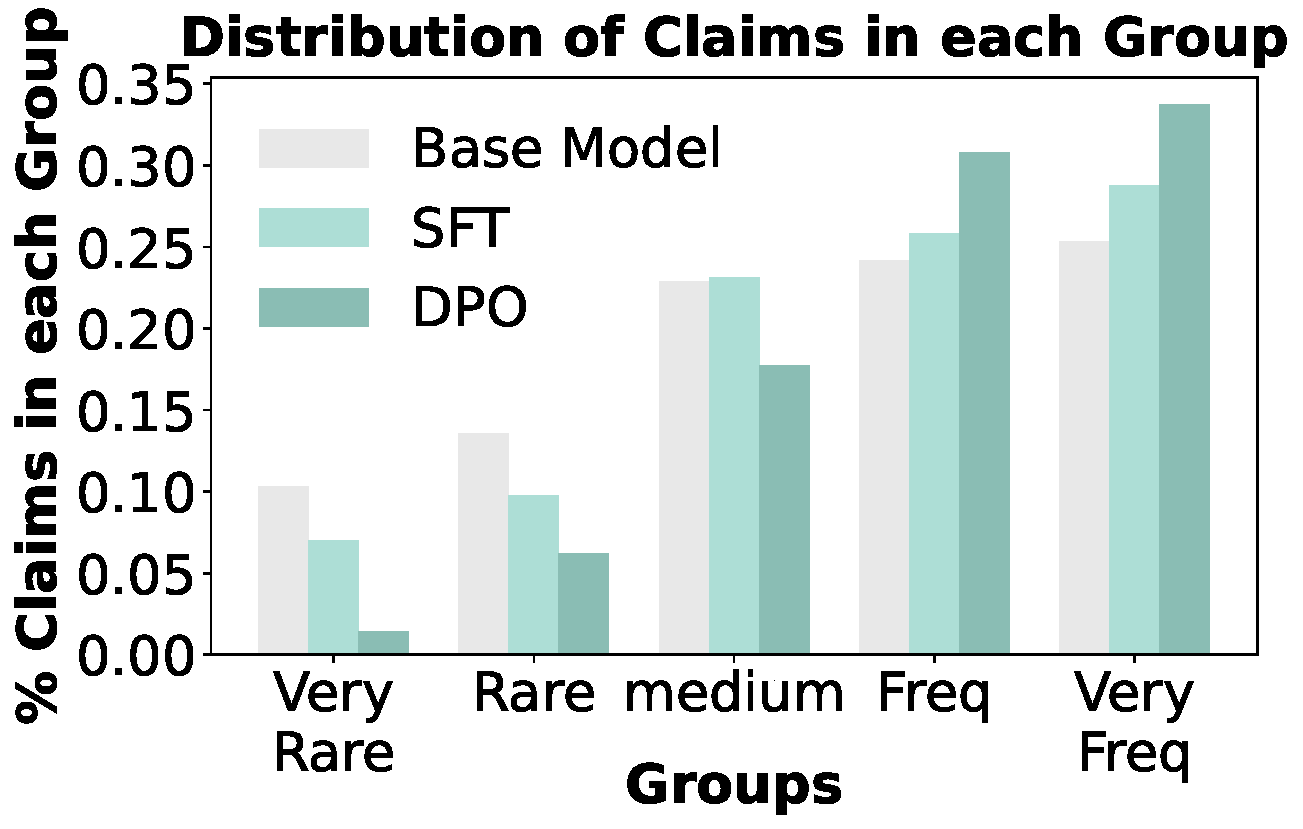
\includegraphics[width=\textwidth]{FenCE_figures/distribution_claims_by_group.pdf}
    \caption{Distribution of claims}
    \label{fig:response_shift_distribution_claims}
  \end{subfigure}
  \begin{subfigure}[b]{0.32\textwidth}
    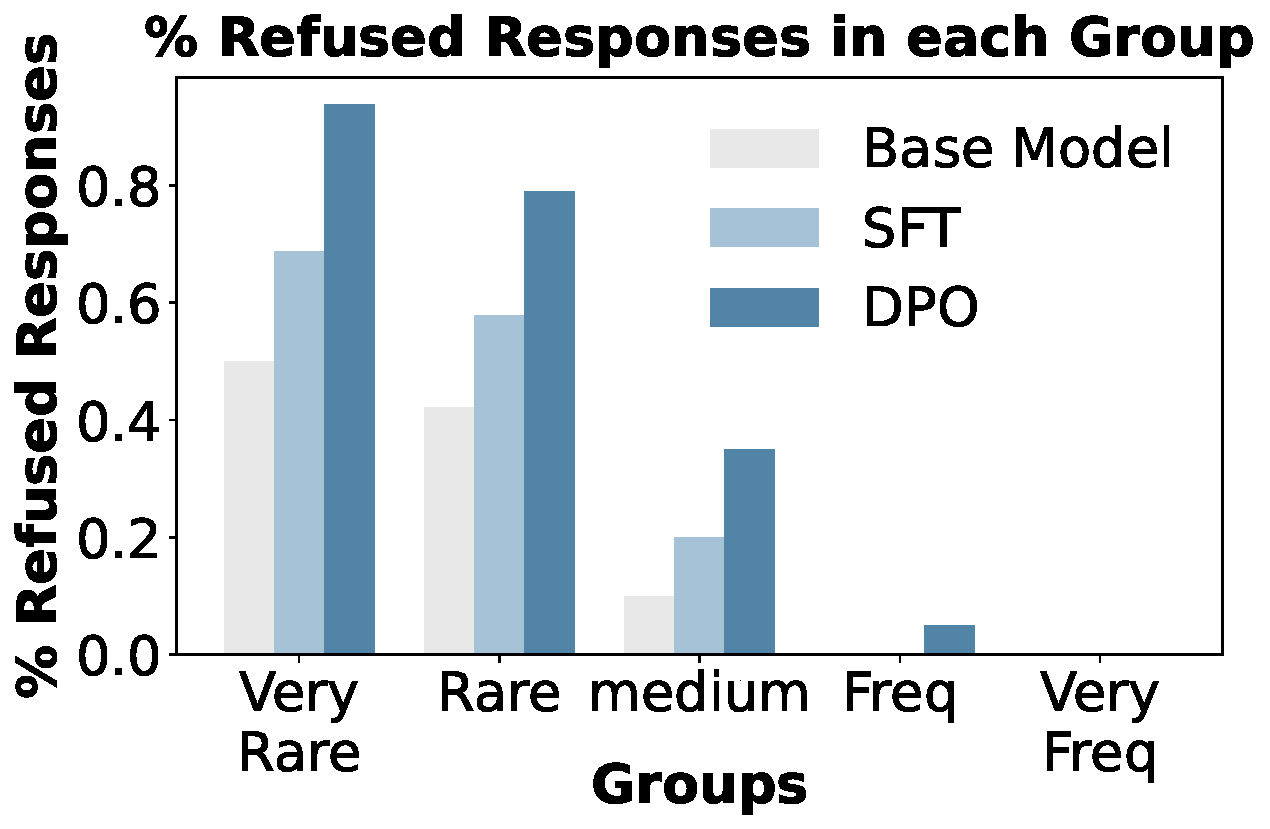
\includegraphics[width=\textwidth]{FenCE_figures/percent_refused_responses_by_group.pdf}
    \caption{\% Refused responses}
    \label{fig:response_shift_refused_responses}
  \end{subfigure}
  \begin{subfigure}[b]{0.32\textwidth}
    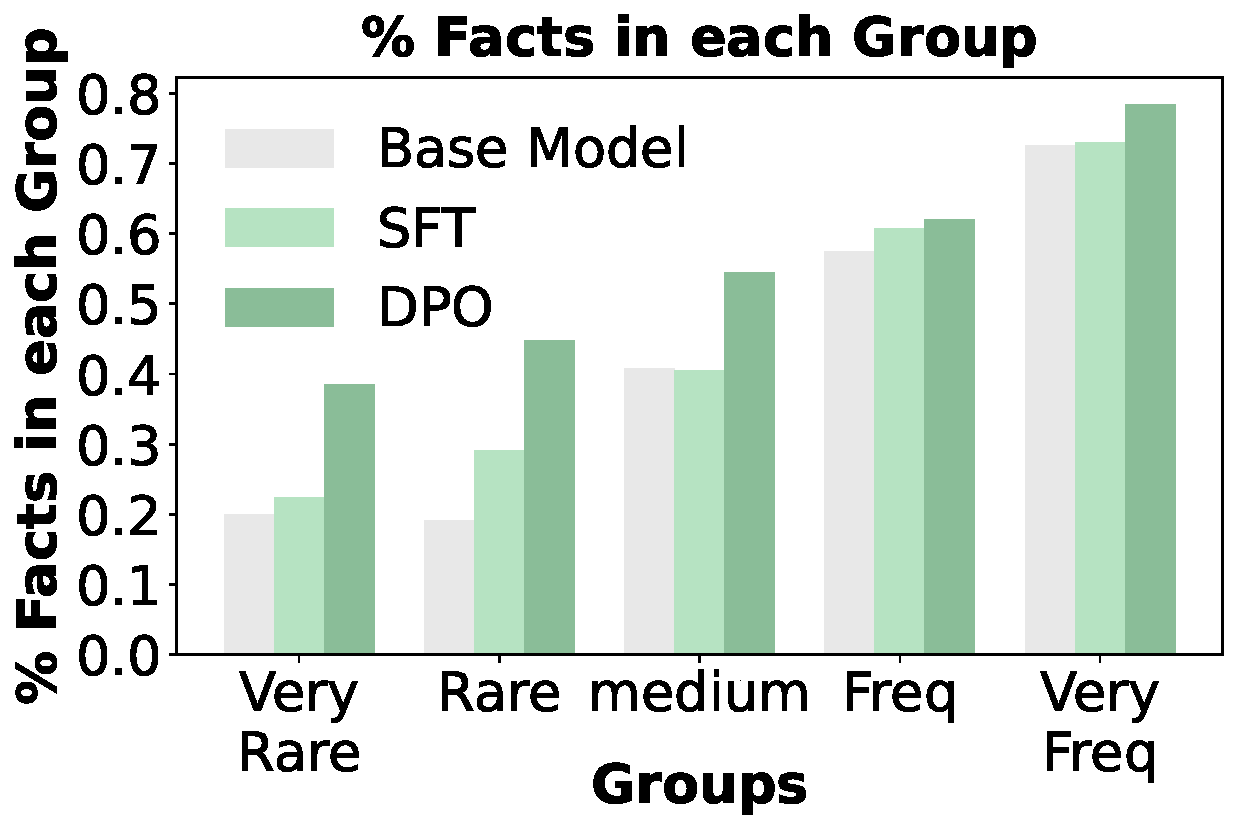
\includegraphics[width=\textwidth]{FenCE_figures/percent_facts_by_group.pdf}
    \caption{\% Facts}
    \label{fig:response_shift_num_facts}
  \end{subfigure}
  
  \caption{Statistics of generated responses, where we group the prompts by the popularity of the person to write biography for, as labeled in the FActScore dataset. We compare zero-shot Llama3-8B-chat (denoted as \textit{``Base Model''}), SFT + \fencemodelname (\textit{``SFT''}), and our method, Edit/Remove + Coarse (\textit{``DPO''}).}
  \label{fig:response_shift}
\end{figure*}

\begin{figure}[t]
    \centering
    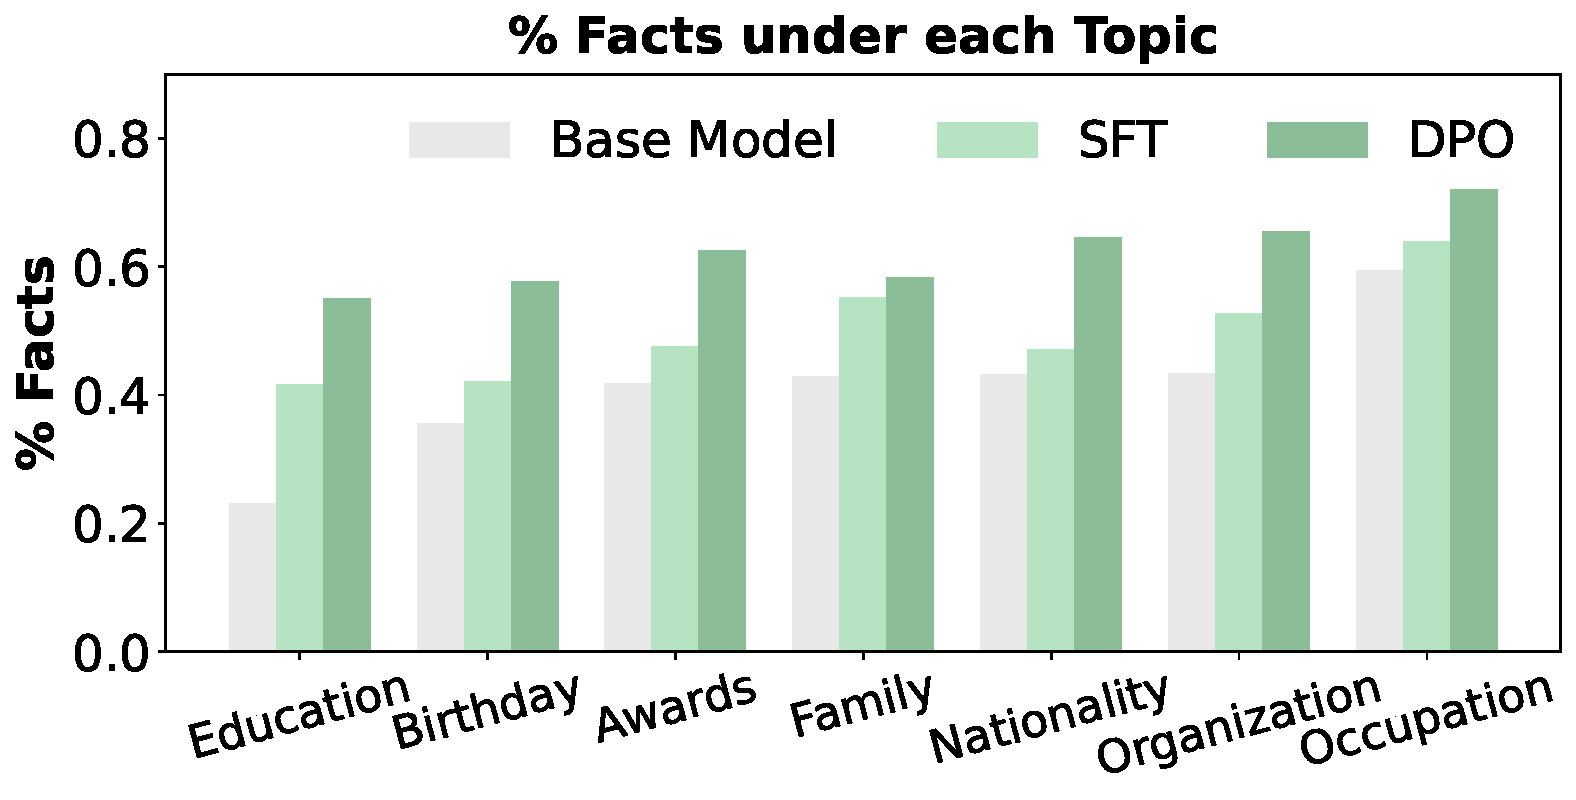
\includegraphics[width=0.7\linewidth]{FenCE_figures/facts_by_cat.pdf}
    \upv
    \caption{The factuality of claims with different topics, where we pre-define the topics and use Llama3-70B-chat to predict whether each claim covers any topic(s).}
    \label{fig:claim_acc_by_cat}
    \downv
\end{figure}



\start{Baselines and Ablations}
We implement four baselines: SFT, FactTune-FS~\citep{FactTune}, Self-Eval-SKT~\cite{self-eval-skt}, and EVER-Pref~\citep{EVER}. 
All methods sample $N$ candidate responses for each training prompt.
SFT first uses the generator itself to score responses by computing the percentage of factual claims and finetunes with the best response.
FactTune-FS first finetunes on all candidates and then uses all $\binom{N}{2}$ candidate pairs as DPO pairs, preferring the one with a higher score based on retrieved context.
Self-Eval-SKT self-trains an evaluator using the model's own knowledge and uses the evaluator to score responses with no external context, also resulting in $\binom{N}{2}$ preference pairs.
EVER-Pref uses all $N$ candidates as rejected responses and constructs a preferred response by iteratively evaluating and correcting false information in each passage.

For ablations, we first equip SFT, FactTune, and EVER with our evaluator, \fencemodelname, and the three external tools, denoted as ``SFT + \fencemodelname'', ``Coarse'', and ``Edit'' in \autoref{tab:res-ablation}, respectively. 
Then we implement ``Edit + Coarse'', which corrects all false information without checking whether it corresponds to a lesser-known fact.
We denote our full method as ``E/R + Coarse'' (Edit/Remove + Coarse).
% More implementation details can be found in \S\ref{sec:implementation_details}.

Note that we do not compare to retrieval-augmented (RAG) methods~\cite{RAG} because it is not a fair comparison. RAG-based methods require access to external knowledge sources or tools in inference, while in our experiments, we only used ``\texttt{tell me a bio of <entity>}'' as the prompt. 
Furthermore, while most RAG-based methods aim to improve the understanding of the long retrieved context, our main focus is to train the model to better utilize the knowledge it has seen during pretraining.

We also do not compare to inference-time methods~\cite{ITI,DoLA} because these methods need to call the model multiple times in inference, introducing heavy latency issues. In the real world, such latency is unacceptable in production. In comparison, our method uses the standard random decoding in inference and does not introduce extra inference-time cost. Furthermore, in principle, our method is orthogonal to those inference-time methods and can be combined.


\begin{figure}[t]
  \centering
  % \hspace{-0.4cm}
  \begin{subfigure}[b]{0.4\textwidth}
    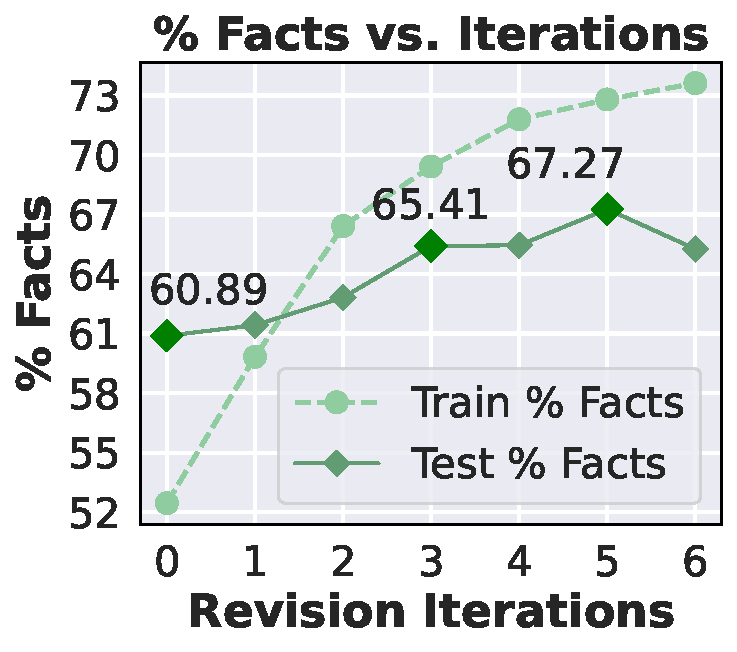
\includegraphics[width=\textwidth]{FenCE_figures/hyper_param.pdf}
    % \vspace{-0.5cm}
    \caption{Iterations of Revision}
    \label{fig:hyper_param_iter}
  \end{subfigure}
  \hspace{0.4cm}
  \begin{subfigure}[b]{0.375\textwidth}
    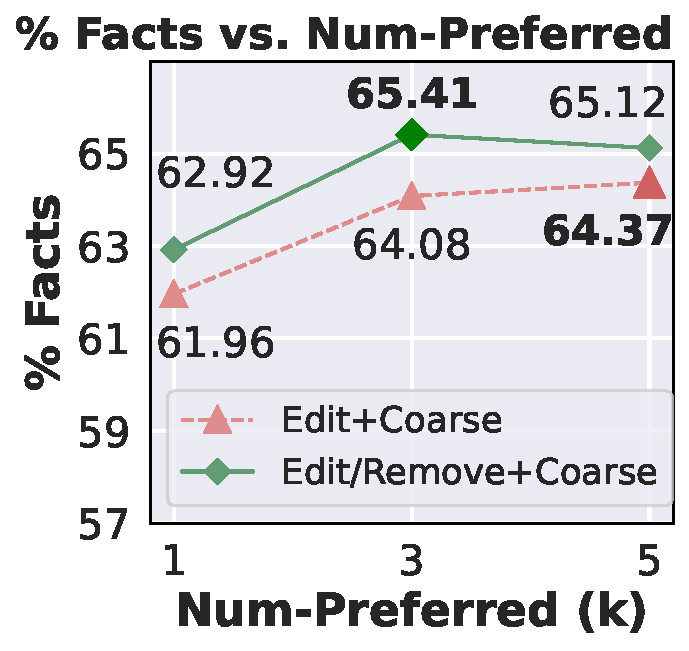
\includegraphics[width=\textwidth]{FenCE_figures/hyper_param_topk.pdf}
    % \vspace{-0.5cm}
    \caption{top-$k$}
    \label{fig:hyper_param_k}
  \end{subfigure}
  \caption{Hyper-parameter analysis. We investigate how percentage of facts changes
  (a) as number of iterations to revise candidate responses increases, and 
  (b) with different numbers of preferred responses for each prompt.
  }
  \label{fig:hyper-param}
\end{figure}

\subsection{Main Results}
Results in \autoref{tab:res-factscore} answer (\textbf{RQ2}) and show that our method significantly improves Llama2/Llama3's factuality by 16.85/14.45\% on FActScore and 17.64\%/8.25\% on TruthfulQA.
Results also show that our method significantly outperforms the best baseline on factuality training (e.g., by 8.83/6.96\% on FActScore for Llama2/Llama3).

\autoref{tab:res-ablation} presents the ablations with \fencemodelname as the evaluator.
The comparison between using \fencemodelname and Llama3-8B-chat shows that \fencemodelname can improve the performance of SFT, EVER-Pref, and FactTune-FS, which emphasizes the significance of training factuality evaluator models.
For example, SFT with \fencemodelname as the evaluator outperforms SFT with Llama3 as the evaluator by 3.74\%.
In addition, we also observe that our method of combining response editing/removing with coarse-level scoring achieves significantly better performance.
% In particular, our full method, which only corrects false information with common facts, outperforms ``Edit + Coarse'', which could introduce both common and lesser-known facts into the training data.
The above results answer (\textbf{RQ3}), demonstrating the effectiveness of our training recipe.






\subsection{Result Analyses}

\start{Distribution of Generated Claims}
We first group the prompts by the popularity of the person to write biography for, which is provided as meta data in the FActScore dataset, and then compare the distribution of generated claims in each group before and after training.
As shown in \autoref{fig:response_shift_distribution_claims}, after training, the generator outputs less information for unfamiliar people and outputs more information for popular ones, suggesting that it learns to only generate information that is likely to be factual.

In addition, as shown in \autoref{fig:response_shift_refused_responses}, we observe that the generator refuses to generate responses more frequently for rare entities (e.g., by generating ``I apologize, but I'm not familiar with this person.''), and almost never refuses for frequent ones. 
This aligns with previous research's conclusion~\citep{unfamiliar-finetuning} that training the model to say ``I don't know'' to unfamiliar prompts reduces hallucination.


\start{Performance Breakdown}
We further check the generator's performance (i.e., percentage of factual claims) on different groups of prompts. 
As shown in \autoref{fig:response_shift_num_facts}, we observe that our method achieves consistent performance gain over all groups of prompts, which is another reason why our method obtains higher overall performance.

Similarly, we check the performance on claims describing different topics, where we first come up with a list of topics and then prompts Llama3-70B-chat to determine whether each claim covers any of the topics. 
In \autoref{fig:claim_acc_by_cat}, our method generates more factual claims under all the topics, and the performance gain is larger on unfamiliar topics (i.e., topics where the generator has lower scores). 

\start{Hyper-parameter Analysis}
We first alternate the number of iterations to revise the responses and inspect the testing and training accuracy (i.e., the average \% of facts of the best preferred responses).
As shown in \autoref{fig:hyper_param_iter}, with more revision iterations, we can always obtain preferred responses with better factuality, but the test performance converges after the third iteration. 
In other words, training data with fewer factual errors does not always transfer to better test performance.


In our experiments, we only choose the top-$k$ candidates (ranked by the percentage of facts) as preferred responses. We investigate the effect of $k$ in \autoref{fig:hyper_param_k}. We observe that training on top-3 and top-5 responses leads to similar performance. With all the $k$s in our experiments, our method consistently outperforms the ``Edit + Coarse'' ablation.




% \section{Related Work}
% \start{Factuality Evaluation} To judge the factuality of long-form model responses, recent works have presented fine-grained level evaluation frameworks that judge each piece of generated fact individually~\citep{factscore,factool,doclens,longform}.
% Such frameworks generally leverage an LM evaluator to make judgments.

% To train LM evaluators, one line of work constructs new training datasets by collecting human judgement~\citep{alpaca_eval,TIGERScore}. 
% Another line of work distills open-source evaluators from proprietary models such as GPT-4, training the evaluator to generate textual critique~\citep{shepherd,ultrafeedback,AutoJ} or fine-grained judgment~\citep{prometheus,FAVA}.
% A recent work \citep{FLAMe} leverages a combination of existing public datasets to train an evaluator.
% We further augment the public datasets with more diverse knowledge sources and more informative judgment feedback.


% \start{Enhancing Generator's Factuality}
% To reduce hallucinations, previous works present inference-time methods, including re-computing token probabilities~\cite{CAD,DoLA} or conducting post-editing~\cite{self-critiquing,self-improve,self-correct,self-refine,CRITIC,FAVA}. Such methods inevitably suffer from latency issues.

% Another approach is to train the model for factuality. Following general reward modeling methods that produce a score for the entire response~\citep{RLHF,InstructGPT,RLHF-QA}, FactTune \citep{FactTune} trains the generator by preferring responses with higher percentage of facts, which is limited by the generator's capability. 
% EVER~\citep{EVER} constructs high-quality responses by correcting false information, which may introduce lesser-known facts and could potentially harm model factuality~\citep{understand-finetuning}.
% Both methods either prompt proprietary model or use the generator itself to evaluate its own factuality, which are either restricted by terms of use or suffer from self-bias.

% Our method is different from existing methods in the following aspects: (1) we combine response revision and scoring to construct high-quality responses while ensuring the correctness of preference ranking, (2) we only correct false information with common facts and remove other misinformation from training, and (3) we use our open-source evaluator, \fencemodelname, for both revision and scoring.




\section{Chapter Summary}
In this chapter, we improve LM generators' factuality by training an open-source evaluator model, \fencemodelname.
To train \fencemodelname to leverage diverse knowledge sources and to generate more informative feedback, 
we equip a combination of public datasets with textual critique along with judgment scores and obtain additional source documents by calling a multiplicity of tools.
We then present a training recipe that leverages \fencemodelname to finetune LM generators for better factuality, where we construct preference data by prompting \fencemodelname to revise and score the generator's responses, without introducing lesser-known facts in training.
Experiments show that \fencemodelname outperforms strong proprietary models such as Claude-3 on LLM-AggreFact.
Our factuality training method improves Llama3-8B-chat's factuality performance by 14.45\% on FActScore and 8.25\% on TruthfulQA.

\autoref{chap:prm-training} adapts the high-level idea of auxiliary model training to coding agent, where we first show that the coding agent performs better in inference if it receives critique from an auxiliary model every $k$ steps. Then, we propose a data construction method to train an open-source critique model. 



\begin{table*}[!t]
\centering

\resizebox{\textwidth}{!}{
\begin{tabular}{p{20.1cm}}
\toprule
\dlrow \textit{\textbf{Source Document} (Dataset: FRANK-xsum)}  \\
Title: News Articles \\
Text: They believe ministers are placing too much emphasis on the environment at the expense of trees grown for timber.
Britain is currently the world's third largest importer of wood.
Ministers said they were encouraging commercial forestry organisations to invest in woodland creation.
Conifer forests have been a familiar sight for half a century in Wales and have helped the timber industry grow.
But Confor, which promotes the forestry industry, warns that at least 16,000 hectares - or 40,000 acres - of commercial forest have been lost since 2001 and need to be re-planted to meet needs.
Half of the woodland is managed by Natural Resources Wales with the the other half by private companies.
As an industry, it is estimated to be worth more than £450m a year to the Welsh economy.
But there is a conflict with environmental policy.
\textbf{Successive ministers have wanted more native, broadleaf species of trees and better access for walkers and bike riders while conservationists claim commercial forests are bad for wildlife.}
However, some forests in Wales are difficult to reach and hard to harvest while transporting the timber through rural communities can bring companies into conflict with local residents.
The Welsh government wants a balance between the environmental, the economic and the social in how forestry is developed.
It points to its Glastir scheme which encourages farmers and other landowners to plant woodland.
It said its Woodlands for Wales forestry strategy "sets out how we want Wales to be known for its high quality woodlands that enhance the landscape, provide real social and community benefits, support thriving woodland-based industries and contribute to a better quality environment".
Martin Bishop, of Confor, which represents 200 businesses in Wales, believes the emphasis on environmental aspects is seen as "sexier" than commercial forestry.
He said the current system is also too bureaucratic for creating new woodland areas.
Mr Bishop said 90 hectares were planted last year but there needed to be 20,000 hectares a year to meet long-term targets set by ministers.
"There's a huge market for our timber. Every saw miller tells me he would double or treble production if the timber was there to feed that mill," he added. \\
\\
\midrule 

\dlrow \textit{\textbf{Claim}} \\
Conservationists are calling for a national project to protect forests in wales. \\
\\
\dlrow \textit{\textbf{Ground Truth Label}} \\
\colorR{Non-Factual} \\
\\
\midrule

\blrow \textit{\textbf{Our Generated Critique and Label}} \\
\textbf{Critique}: The document does not mention conservationists calling for a national project to protect forests in Wales. It only mentions that conservationists claim commercial forests are bad for wildlife, but it does not mention a specific call for a national project. \\
\\
\textbf{Label}: \colorR{Unverified} \\
\bottomrule
\end{tabular}
}
% \vspace{-0.05cm}
\caption{An example of the textual critique we generate. We highlight the most relevant sentence in the document. In this case, our generated critique aligns with the judgment label.
}
\label{tab:case_1}
% \vspace{-0.2cm}
\end{table*}




\begin{table*}[!t]
\centering

\resizebox{\textwidth}{!}{
\begin{tabular}{p{24cm}}
\toprule
\dlrow \textit{\textbf{Original Source Document} (Dataset: FRANK-CNN/DM)}  \\ 
Title: News Articles \\
Text: (CNN) Deputies rushed Kenneth Morgan Stancil III from court Thursday after the 20-year-old murder suspect swore at a judge and tried to flip over a table. Stancil is accused of killing an employee Monday at Wayne Community College in Goldsboro, North Carolina. Relatives have said victim Ron Lane was gay, CNN affiliate WNCN reported, and investigators are looking into whether the shooting was a hate crime. Authorities arrested Stancil after he was found sleeping on a Florida beach on Tuesday. Just a few minutes into Thursday's hearing on the first-degree murder charge he faces, Stancil snapped back at the judge after he was offered a court-appointed lawyer. \"No, I don't need one,\" said Stancil, who stood before the judge with his legs shackled and his arms handcuffed in front of him. \"You know what I'm saying? I knew I would get life anyway.\" Superior Court Judge Arnold O. Jones interjected, pointing out that the maximum sentence Stancil faces is the death penalty. \"Yes, I know that,\" Stancil fired back. \"But when I knew what I had to do and I knew when I got caught, you know, I knew in my mind that I could get life, I could get the death penalty. You know what I'm saying? Do you follow my topic? I would have killed you, you know what I'm saying, if you're a f---ing child molester.\" The judge told him not to swear. \"I don't give a f--- what you want,\" Stancil said, lunging forward and lifting up the table in front of him. Deputies quickly corralled him and hustled him from the courtroom. The hearing resumed about 25 minutes later, when Stancil was brought back into the courtroom, this time with his arms handcuffed behind him. When asked again by Jones whether he wanted a lawyer, his response was quick -- and calm. \"Yes, sir,\" he said. In an interview with CNN affiliate WRAL, Stancil described himself as a neo-Nazi and said he hates gay people \"with a passion.\" Stancil had worked for Lane, the school's print shop operator, as part of a work-study program, but was let go from the program in early March because of poor attendance, college officials said. \\
\\
\midrule 

\dlrow \textit{\textbf{Claim}} \\
Kenneth Morgan Stancil is accused of killing an employee at Wayne Community College in Goldsboro, North Carolina. \\
\\
\dlrow \textit{\textbf{Ground Truth Label}} \\
\colorG{Factual} \\
\\
\midrule

\blrow \textit{\textbf{Generated Queries to Call the Tools}} \\
\textbf{Search query for Bing Search API}: Kenneth Morgan Stancil Wayne Community College killing \\
\textbf{Queries for Wikipedia}: Kenneth Morgan Stancil; List of school shootings in the United States; Wayne Community College; \\
\textbf{Entities for Google Knowledge Graph API}: Kenneth Morgan Stancil \\
\\
\midrule

\blrow \textit{\textbf{Tool-extracted Source Documents} (after Reranking)} \\
Title: Wayne Community College shooter gets life sentence without parole \\
Text: GOLDSBORO, North Carolina (WTVD) -- \textbf{Kenneth Morgan Stancil III was sentenced Tuesday to life in prison without parole for the murder of 44-year-old Ron Lane on the campus of Wayne Community College in Goldsboro on April 13, 2015.}
Stancil entered the campus print shop on the third floor of the same building that houses the school library and cafeteria shortly after Lane arrived for work that day and shot him once with a pistol-grip 12-gauge shotgun.
...
\\
\\
Title: Stancil guilty in Wayne Community College murder trial - CBS17.com \\
Text: GOLDSBORO, N.C. (WNCN) – After deliberating for an hour and a half, \textbf{a Wayne County jury found Kenneth Morgan Stancil III guilty of first-degree murder.}
He will spend the rest of his life in prison.
During his closing argument Tuesday in a Wayne County court, the district attorney relied largely on Stancil’s own words, \textbf{painting him as confident and proud about his decision to kill a man at Wayne Community College.}
In his counterargument, Stancil’s attorney said the prosecution tried to scare the jury with Stancil’s possession of knives, guns, and white supremacist memorabilia, as well as his numerous tattoos. None of that proved he planned to commit the murder, the defense said.
\textbf{Neither side disputed that Stancil killed Ron Lane at Wayne Community College in 2015}. The prosecution contends it was first-degree murder, but the defense argues ...
\\
\\
Title: Man convicted in fatal Wayne Community College shooting - WRAL ... \\
Text: Man convicted in fatal Wayne Community College shooting
A white supremacist was sentenced Tuesday to life in prison without parole for gunning down a print shop operator at Wayne Community College two years ago.
\textbf{Jurors deliberated for about 90 minutes before convicting Kenneth Morgan Stancil III, 22, of first-degree murder in the April 13, 2015, death of Ron Lane in the school's library.}
Authorities said Stancil shot Lane with a 12-gauge pump shotgun before fleeing the area on a motorcycle. He was captured the next morning when police found him asleep on a beach in Volusia County, Fla.
...
\\
\\
Title: Wayne Community College killing suspect makes shocking allegations in ... \\
... \\
\midrule

\blrow \textit{\textbf{Our Generated Critique and Label}} \\
\textbf{Critique}: The statement is supported by the document. In all the documents, it is mentioned that Kenneth Morgan Stancil III is accused of killing Ron Lane, an employee at Wayne Community College in Goldsboro, North Carolina. \\
\\
\textbf{Label}: \colorG{Supported} \\
\bottomrule
\end{tabular}
}
% \vspace{-0.05cm}
\caption{An example where we obtain multiple relevant source documents by calling a multiplicity of tools.
}
\label{tab:case_2}
% \vspace{-0.2cm}
\end{table*}




\begin{table*}[!t]
\centering

\resizebox{\textwidth}{!}{
\begin{tabular}{p{21cm}}
\toprule
\dlrow \textit{\textbf{Original Source Document} (Dataset: FActScore)}  \\ 
Title: Chadwick Boseman \\
Text: Chadwick Boseman Chadwick Aaron Boseman \textbf{(; November 29, 1976August 28, 2020)} was an American actor. During his two-decade career, Boseman received multiple accolades, including two Screen Actors Guild Awards, a Golden Globe Award, a Critics' Choice Movie Award, a Primetime Emmy Award, and an Academy Award nomination. After studying directing at Howard University, Boseman began his career in theatre, winning a Drama League Directing Fellowship and an acting AUDELCO ...
\\
\\
\midrule 

\dlrow \textit{\textbf{Claim}} \\
Chadwick Boseman was born on November 29, 1977. \\
\\
\dlrow \textit{\textbf{Ground Truth Label}} \\
\colorR{Non-Factual} \\
\\
\midrule

\blrow \textit{\textbf{Generated Queries to Call the Tools}} \\
\textbf{Search query for Bing Search API}: Chadwick Boseman date of birth \\
\textbf{Queries for Wikipedia}: Chadwick Boseman \\
\textbf{Entities for Google Knowledge Graph API}: Chadwick Boseman Stancil \\
\\
\midrule

\blrow \textit{\textbf{Tool-extracted Source Documents} (after Reranking)} \\
Title: knowledge graph result \\
Text: Chadwick Boseman: American actor. Chadwick Aaron Boseman was an American actor, known for portraying African-American historical figures and the fictional African superhero Black Panther. \textbf{Chadwick Boseman Born: November 29, 1976, Anderson, SC.} Chadwick Boseman Died: August 28, 2020 (age 43\u00a0years), Los Angeles, CA. Chadwick Boseman Spouse: Taylor Simone Ledward. Chadwick Boseman Height: 6\u2032 0\u2033. Chadwick Boseman Parents: Leroy Boseman and Carolyn Boseman. Chadwick Boseman Alma mater: Howard University (BFA).
...
\\
\\
Title: Chadwick Boseman | Biography, Movies, Black Panther, \& Death
text: Chadwick Boseman \\
Text: Our editors will review what you’ve submitted and determine whether to revise the article. \\
- Chadwick Aaron Boseman \\
\textbf{- Born: November 29, 1976, Anderson, South Carolina, U.S.} \\
- Died: August 28, 2020, Los Angeles, California (aged 43) \\
- Notable Family Members: son of Leroy Boseman ... \\
Chadwick Boseman (born November 29, 1976, Anderson, South Carolina, U.S.—died August 28, 2020, Los Angeles, California) was an American actor and playwright who became a highly respected movie star with several iconic roles, notably that of T’Challa/Black Panther in the groundbreaking film Black Panther (2018).
...
\\
\\
Title: Chadwick Boseman - Wikipedia \\
Text: Chadwick Boseman Chadwick Aaron Boseman \textbf{(; November 29, 1976August 28, 2020)} was an American actor. During his two-decade career, Boseman received multiple accolades, including two Screen Actors Guild Awards, a Golden Globe Award, a Critics' Choice Movie Award, a Primetime Emmy Award, and an Academy Award nomination. After studying directing at Howard University, Boseman began his career in theatre, winning a Drama League Directing Fellowship and an acting AUDELCO ...
\\
\\
Title: Chadwick Boseman | Biography, Movies, Black Panther, \& Death ... \\
... \\
\midrule

\blrow \textit{\textbf{Our Generated Critique and Label}} \\
\textbf{Critique}: The statement claims that Chadwick Boseman was born on November 29, 1977. However, all four documents consistently state that Chadwick Boseman was born on November 29, 1976, not 1977. \\
\\
\textbf{Label}: \colorR{Contradictory} \\
\bottomrule
\end{tabular}
}
% \vspace{-0.05cm}
\caption{An example where we obtain multiple relevant source documents by calling a multiplicity of tools. The tool-extracted documents all contain the information about Chadwick's birthday, but have diverse formats.
}
\label{tab:case_3}
% \vspace{-0.2cm}
\end{table*}









\chapter{Improving Coding Agent Effectiveness by Training a Critique Model \textcolor{mediumgreen}{(\textit{proposed})}}
\label{chap:prm-training}

\section{Overview}
Synthetic data has proven effective for training coding agents~\cite{swe-smith,R2EGym,hybrid-gym}. However, as in many machine learning settings, the effectiveness of a coding agent is ultimately bottlenecked by the capacity of its base model. Prior work~\cite{swe-smith} shows that, when using Qwen2.5Coder-14B as the base model, coding-agent performance already saturates after roughly 800 training trajectories.

To overcome this limitation, we propose training an auxiliary model to assist the coding agent at inference time. Similar to \autoref{chap:fence}, an ideal auxiliary model should satisfy two properties: (1) it should provide additional performance gains when paired with the primary coding agent, and (2) it should develop capabilities that differ from those of the main coding agent, allowing the two models to be optimized for distinct objectives.

In this chapter, we show that a critique model trained to provide free-form textual feedback to the main model during inference satisfies both criteria for coding-agent tasks. Using a strong critique model such as Claude-Sonnet-4.6, we improve the performance of CWM-32B~\cite{cwm} on SWE-Bench Verified-mini~\cite{swebench} from 29.4\% to 61.0\%. Moreover, we find that using a model fine-tuned for coding-agent tasks, such as SWE-Smith-7B~\cite{swe-smith}, as the critique model does not yield additional gains beyond those achieved by the coding agent alone. This suggests that the critique model requires a different set of capabilities and should be optimized differently from the coding agent itself.

Because using a frontier model as the critique model, such as Claude-Sonnet-4.6, remains expensive at inference time, our \textcolor{aquablue}{\textbf{preliminary experiments}} focus on constructing synthetic data to distill a more cost-efficient critique model, such as Qwen3-8B, that can provide free-form textual critiques to assist the main coding agent during inference. Specifically, we distill Qwen3-8B from Claude-generated critiques using standard supervised fine-tuning (SFT), and this already improves CWM-32B's performance on SWE-Bench Verified from 29.4\% to 33.4\%.

However, we observe that the fine-tuned critique model does not fully reproduce the behavior of the frontier critique model. In particular, its critiques tend to be more verbose, repeating, and contain more unnecessary details, which can distract the main coding agent. These distractions often lead the agent to take unnecessary actions and exhaust the budget of action steps before producing a valid code patch.
In particular, we observe that the vanilla coding agent generates an non-empty code patch for 89.0\% of the examples in SWE-Bench Verified, but when paired with the SFT critique model, the non-empty rate is significantly reduced to 73.4\%.
This indicates that reducing distracting critiques and improving the non-empty rate could be a promising direction to further improve the performance of the system.

Motivated by these observations, we \textcolor{mediumgreen}{\textbf{propose}} to (1) systematically analyze the characteristics of distracting critiques that lead to unnecessary actions, and (2) construct direct preference optimization (DPO) data to further improve the critique model by encouraging it to generate fewer distracting critiques.


\section{Preliminary Experiments}
In our preliminary experiments, we first show that a strong critique model can bring substantial performance gains to the coding agent in inference (\S\ref{sec:prm-strong}).
Then we show that we can further train a more cost-efficient critique model (e.g., Qwen3-8B) by distilling it from the strong critique model (e.g., Claude-Sonnet-4.6) using vanilla supervised-finetuning (SFT) (\S\ref{sec:prm-sft}).
Finally, we reveal the remaining gaps between the student critique model and the teacher critique model, which motivates our proposed method (\S\ref{sec:prm-proposed}).

\subsection{Inference-time Critique Models can be Effective}
\label{sec:prm-strong}

\start{Experimental Setup}
We experiment with the SWE-Bench Verified dataset~\cite{swebench} with mini-SWE-Agent as the infrastructure~\cite{sweagent}. We use CWM-32B~\cite{cwm} as the coding agent and experiment with three critique models: a frontier model, Claude-Sonnet-4.6~\cite{claude46}, a cost-efficient open-source model, Qwen3-8B~\cite{qwen3}, and a model finetuned for coding agent tasks, SWE-Smith-7B~\cite{swe-smith}.

Following previous work~\cite{swe-prm}, we adopt the setting where the critique model provides free-form textual critique for the main coding agent every $k$ steps during inference. We use $k=5$ in our experiments. The coding agent can perform at most $150$ steps. After exceeding the limit, the process will be terminated, even if no coding patch is generated.

We prompt the critique model to include (1) error analysis for the current trajectory, (2) high-level instructions for completing the task, and (3) the reasoning process for generating the critique, which is shown to be effective empirically~\cite{swe-prm}. 

\start{Experimental Results}
As shown in \autoref{tab:prm:prelim}, we observe that:
(1) The frontier critique model (Claude-Sonnet-4.6) can bring substantial performance gains to the coding agent, improving the resolved rate from 29.4\% to 61.0\%.
(2) Using a weak critique model such as Qwen3-8B may even reduce the performance of the coding agent, but the performance loss is not significant.
(3) The model finetuned for coding agent tasks (SWE-Smith-7B) is not an effective critique model, which performs even worse than Qwen3-8B. This indicates that the critique model and the coding agent require different capabilities and should be optimized differently.



\begin{table}[t]
  \centering
  \small
  \resizebox{0.6\columnwidth}{!}{%
  \begin{tabular}{l ccc}
  \toprule
  \multirow{2}{*}{\bf Crtique Model} &
  \multicolumn{3}{c}{\bf SWE-Bench Verified} \\
  \cmidrule(lr){2-4}
  & Resolved \% & Non-Empty \% & Avg Steps \\
  \midrule
  \sdlrow & \multicolumn{3}{c}{\textit{Coding Agent: CWM-32B}} \\
  \midrule
  \textemdash & 29.4 & 89.0 & 34.54 \\
  \midrule
  Qwen3-8B & \bad 24.6 & 82.4 & 39.57 \\
  SWE-Smith-7B & \bad 21.2 & 62.2 & 41.07 \\
  Claude-Sonnet-4.6   & \better \bf 61.0 &  90.0 & 30.28 \\
  \midrule
  Qwen3-8B + SFT & \good 33.4 & 73.4 & 61.39 \\
  \quad + fallback & \good 36.4 & 94.8 & \textemdash \\
  \bottomrule
  \end{tabular}%
  }
  \caption{Results on equipping CWM-32B with different critique models on SWE-Bench Verified. ``fallback'' refers to the setting where if the coding agent exceeds the limit, we run inference on this example again without the critique model.}
  \label{tab:prm:prelim}
\end{table}


\subsection{Distilled Critique Models also Bring Performance Gains}
\label{sec:prm-sft}
\start{Experimental Setup}
To reduce inference cost, we distill Qwen3-8B from Claude-Sonnet-4.6 using vanilla supervised-finetuning (SFT).

We build training data from 500 trajectories with CWM-32B as the coding agent and Claude-Sonnet-4.6 as the critique model. For each piece of critique, we use the partial trajectory before it as the prefix and optimize the probability of the critique.

We train the model on 8 L-40 GPUs, with a batch size of 8, and a learning rate of 5e-6. We train the model for 3 epochs.

\start{Experimental Results}
As shown in \autoref{tab:prm:prelim}, we observe that the SFT model can also bring performance gains to the coding agent, improving the resolved rate from 29.4\% to 33.4\%.
However, the performance gap with using the frontier critique model is still large, indicating that there is still a large room for improvement.

\start{The Remaining Gaps}
We observe that one major reason that limits the performance of the SFT-critique model is that is has a much lower non-empty rate than the base coding agent (reducing from 89.0\% to 73.4\%). What happens is that when the critique is distracting, the coding agent performs on average more actions than before (increasing from 34.54 to 61.39). It exceeds the limit of 150 steps more often, where the process is terminated before a valid code patch is generated.

We present a simple fix to the limit-exceeding problem denoted as ``+ fallback'' in \autoref{tab:prm:prelim}. Specifically, when the coding agent exceeds the limit, we start from the first step again and run inference with the coding agent alone, without any critique models. This improves the non-empty rate from 73.4\% to 94.8\% and improves the resolved rate from 33.4\% to 36.4\%.

However, to reduce inference latency, we aim to train the critique model itself to avoid distracting behaviors. In the next section, we propose to systematically investigate the characteristics of the distracting critiques that lead to unnecessary actions, and construct training data to reduce such distracting behaviors.



\section{Proposed Method}
\label{sec:prm-proposed}

\subsection{Analysis of Distracting Critiques}
\start{Proposed Method}
To investigate what types of critiques are distracting and lead to unnecessary actions, we propose to manually check a subset of trajectories where using the SFT critique model exceeds the limit but using Claude-4.6 as the critique model does not, and discover a list of differences between the critiques they generate.

Below is a list of differences that we already observed. Note that the list is not complete and will be updated as we conduct further analysis.
\begin{itemize}
  \item \textbf{The SFT critique model generates more implementation-level suggestions and the frontier model generates more high-level instructions}. For instance, the SFT critique model generates the concrete commands to execute, while the frontier model generates the general plan to locate the relevant files or fix the issue. We observe that when provided with implementation-level guidance, the coding agent tends to follow the exactly same suggestions in the critique. When the critique is distracting, the coding agent performs more unnecessary actions than before and exceeds the limit more often. Furthermore, the training data for the critique model contains much fewer concrete actions than the coding agent model. In this way, it is likely that the critique model has weaker action generation capability than the coding agent, making it unreasonable for the coding agent to follow its suggested actions.
  \item \textbf{The SFT critique model generates more complex critiques that contain more suggestions than the frontier model}. We observe that the SFT critique model tends to generate long critiques, while the frontier model generates shorter critiques and dynamically adjusts its suggestions based on the coding agent's progress.
  \item \textbf{The critique generated by the SFT model does not align well with the coding agent's recent progress}. We observe that there are cases where the SFT critique model generates the same instruction multiple times, even if the coding agent has already completed the first few steps in the instruction. In this way, the coding agent is likely to start over from the first step, stucking in a loop until the step limit is reached.
\end{itemize}

\start{Proposed Experiments}
In the next step, we propose to design controlled experiments to verify our hypothesis that the behaviors mentioned above are indeed harmful to the performance of the coding agent.

Specifically, for each type of behaviors that are potentially distracting, we use a frontier model to detect such critiques during inference. Whenever it observes such behaviors, we prompt the frontier model to revise the critique by removing such behaviors and keeping the remaining parts the same.
Then we compare the performance with the original and revised critiques.
If the revised critiques can bring significant performance gains, we can verify our hypothesis that such behavirors are indeed distracting and should be reduced from the critique.


\subsection{Constructing DPO Data to Distill Critique Models}
\start{Proposed Method}
After identifying the characteristics of the distracting critiques, we can construct directed preference optimization (DPO) data to further improve the performance of the critique model.

Similarly to the proposed analysis, we select ``breakpoints'' in the training trajectory, leverage the SFT critique model to generate multiple critiques, and prompt the frontier model to score the critiques based on whether they avoid the distracting behaviors. We will use the critiques with higher scores as the preferred responses and the critiques with lower scores as the rejected responses, and train the critique model with DPO.



\start{Proposed Experiments}
We expect to find that the DPO-trained critique model can generate fewer distracting critiques and improve the performance of the coding agent.

In particular, we evaluate the performance of coding agents on the SWE-Bench Verified dataset~\cite{swebench} with mini-SWE-Agent as the infrastructure~\cite{sweagent}.
We experiment on two base coding agents: CWM-32B~\cite{cwm} and Qwen2.5Coder-32B~\cite{qwen25coder}.
We expect to see that the performance of using the DPO-trained critique model is significantly better than three baselines and ablations: (1) inference with the coding agent alone, without any critique models,  (2) inference with the untrained model (Qwen3-8B or Qwen2.5Coder-32B) as the critique model, and (3) inference with the SFT-trained critique model.



\chapter{Conclusion}

%\appendix
%\include{appendix}

\backmatter

%\renewcommand{\baselinestretch}{1.0}\normalsize

% By default \bibsection is \chapter*, but we really want this to show
% up in the table of contents and pdf bookmarks.
\renewcommand{\bibsection}{\chapter{\bibname}}
%\newcommand{\bibpreamble}{This text goes between the ``Bibliography''
%  header and the actual list of references}
\bibliographystyle{plainnat}
\bibliography{register} %your bib file

\end{document}